% rubber: setlist arguments --shell-escape

\documentclass[notitlepage,oneside]{book}

\usepackage{fancyhdr}

\usepackage[dvipsnames]{xcolor}
\definecolor{darkcyan}{rgb}{0.0, 0.55, 0.55}
\definecolor{britishracinggreen}{rgb}{0.0, 0.26, 0.15}
\definecolor{ao(english)}{rgb}{0.0, 0.5, 0.0}
\usepackage{tocloft}

\newcommand{\defineauthorcolor}[2]{%
  \colorlet{author#1}{#2}% Create an author colour
  \expandafter\def\csname authoredby#1\endcsname{% Create author colour settings
    \renewcommand{\cftchapfont}{\bfseries\color{author#1}}% Chapter colour
    \renewcommand{\cftsecfont}{\color{author#1}}% Section colour
    \renewcommand{\cftsubsecfont}{\color{author#1}}}% Subsection colour
}
\makeatletter
\newcommand{\authoredby}[1]{\addtocontents{toc}{\protect\@nameuse{authoredby#1}}}%
\makeatother
\defineauthorcolor{A}{blue}% Author A will be coloured red
\defineauthorcolor{B}{ao(english)}% Author B will be coloured blue




\usepackage{framed}

\usepackage[vmarginratio=1:1,a4paper,body={6.5in, 9.5in}]{geometry}

\usepackage[T2A]{fontenc}
\usepackage[utf8]{inputenc}
\usepackage[english]{babel}

\usepackage{wrapfig}

\usepackage{amsmath}
\makeatletter
\renewcommand*\env@matrix[1][\arraystretch]{%
  \edef\arraystretch{#1}%
  \hskip -\arraycolsep
  \let\@ifnextchar\new@ifnextchar
  \array{*\c@MaxMatrixCols c}}
\makeatother


\DeclareMathOperator*{\argmin}{arg\,min}
\DeclareMathOperator*{\argmax}{arg\,max}
\DeclareMathOperator*{\proj}{proj}
\DeclareMathOperator{\Span}{span}
\DeclareMathOperator{\Div}{div}


\usepackage{amssymb}
\usepackage{amsfonts}
\usepackage{amsthm}
\newtheorem{theorem}{Theorem}
\newtheorem{definition}{Definition}

\usepackage{hyperref}
\hypersetup{
linkbordercolor=lightgray
%linkcolor=black
%hidelinks
%    colorlinks=true,% make the links colored
}

\usepackage{graphicx}
\graphicspath{{./img/}}


\usepackage{caption}
\usepackage[newfloat,cache=false]{minted}
\captionsetup[listing]{position=top}
\captionsetup[listing]{skip=-3pt}


\usepackage{colortbl}
\newcommand\TODO[1]{\textcolor{red}{{\bf TODO :} \it #1}}


\makeatletter
\newcommand*{\toccontents}{\@starttoc{toc}}
\makeatother

\setcounter{tocdepth}{0}% Allow only \chapter in ToC

\title{{\Huge Least squares for programmers}\\
{\large with illustrations}\\
\vspace{5mm}
{\large \url{https://github.com/ssloy/least-squares-course/}}
\vspace{5mm}
}
\author{Dmitry Sokolov, Nicolas Ray and Étienne Corman}
\date{Université de Lorraine, CNRS, Inria, LORIA, F-54000 Nancy, France}

\begin{document}


\authoredby{B}
\pagestyle{fancy}
\renewcommand{\chaptermark}[1]{\markboth{#1}{#1}}
\fancyhead[R]{\textcolor{ao(english)}{core text}}
\fancyhead[L]{\chaptername\ \thechapter\ --\ \leftmark}

\maketitle

\vspace{10mm}

\toccontents

\vspace{10mm}
\begin{center}
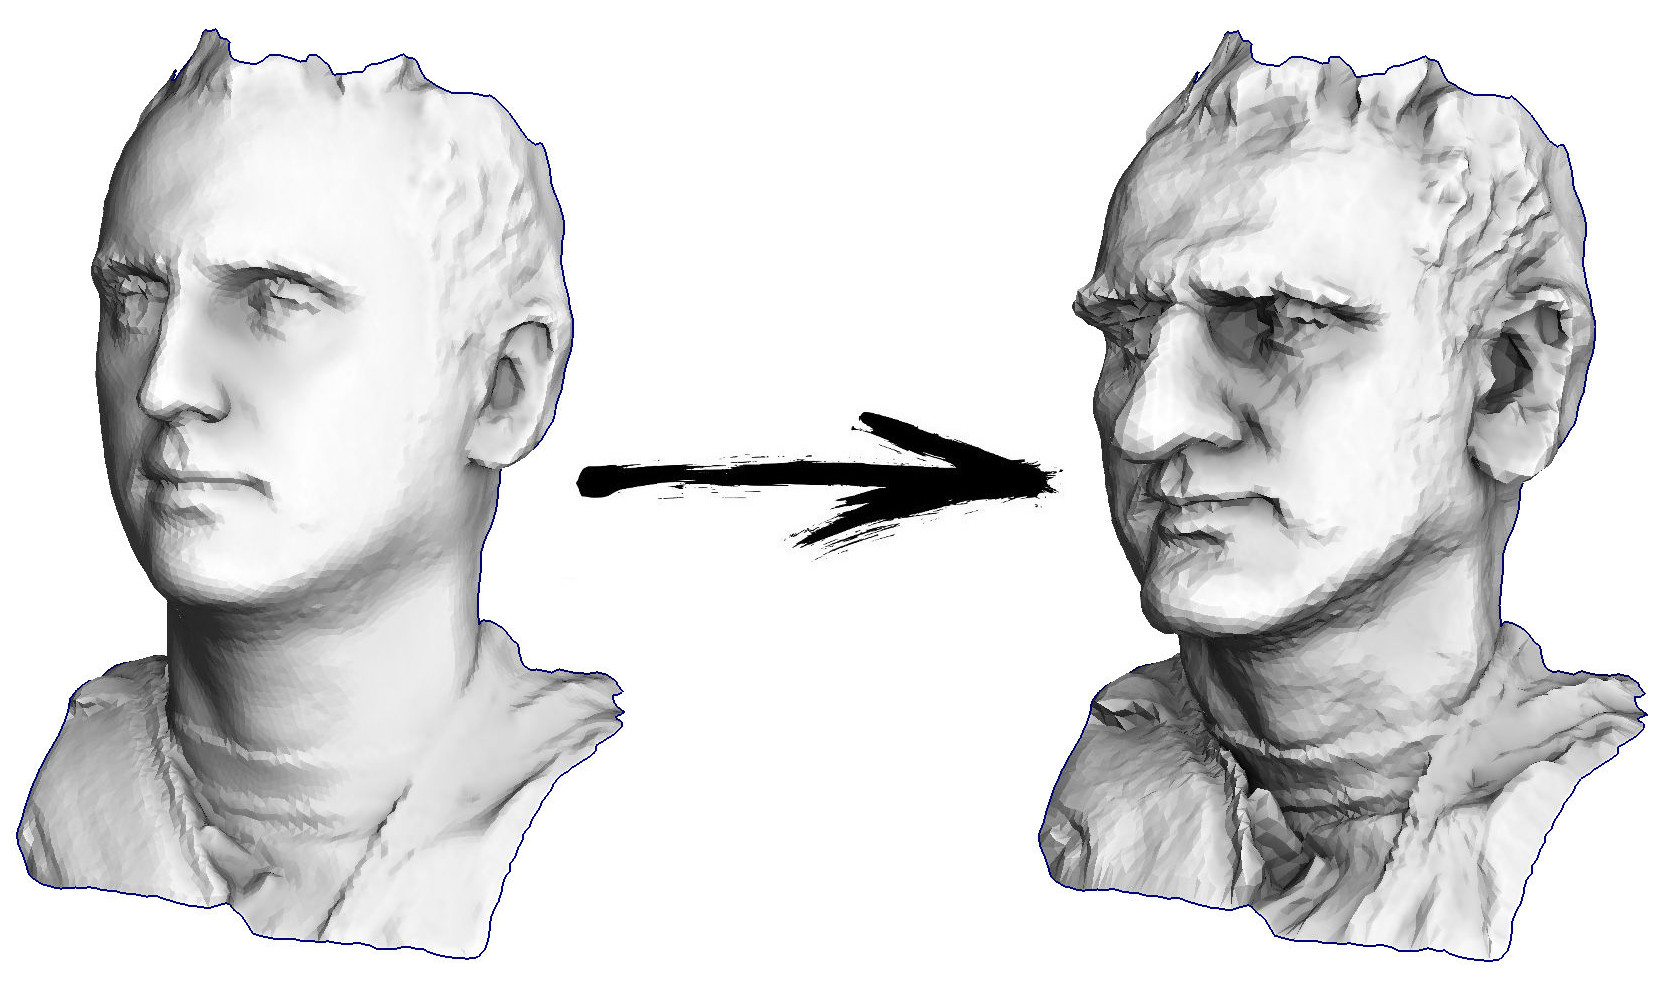
\includegraphics[width=.7\linewidth]{caricature.jpg}
\end{center}

\setcounter{chapter}{-1}
\chapter{The reading guide}
%\addcontentsline{toc}{chapter}{Preface}

%Intended Audience (50 words => 46)
%We present the Least Squares method to manipulate geometric objects (curves, images, surfaces).
%It is a basic (fundamental) of numerical optimization that can be efficiently used by programmers that are not specialized in applied mathematics because it is simple, efficient and general enough to handle a large family of problems.

%Course Prerequisites (50 words)
% Anyone able to program computer graphics algorithms can learn to use least squares with this course. Attendees already using it or having stronger mathematical background may discover some interesting relations with other domains.

%Executive Statement (Maximum 50 words)
% We present how to manipulate geometric objects (curves, images, surfaces) by optimizing their characteristics using least squares methods; it is a very efficient tool that does not require too much mathematical background.


%Course Syllabus
%The course is decomposed in three parts: an introduction of least squares, numerous use cases to demonstrate its usefulness, and the presentation of its strong relations with to adjacent scientific domains.
% * It starts with a gentle introduction of the least squares method, providing some intuitions about linear systems.
% * Then we proceed to the main course: how do we instantiate least squares to solve some problems? What can be the choice of variables? The energy? How to deal with constraints? Are we bound by the linearity?
%   This part is thoroughly illustrated with real examples and comes with simple source code that is meant to be experimented with.
% * The last part provides some insights about the strong connections between the fundamentals of least squares, probability theory, finite element methods and neuronal networks.

%Course rationale
% In computer graphics, many problems can be efficiently solved by numerical optimizations: texture mapping, deformations, physical simulations, morphing, etc.
% These methods come from the applied mathematics community and are not always accessible/mastered by computer science students.
% The purpose of this course is to bring to the audience a first brick of numerical optimization. We choose the least squares method because it does not require strong mathematical background, it is extremely efficient, and can handle many different problems.
% We not only present the mathematical foundation of the method, but also illustrate it with numerous use cases, ranging from 1D function smoothing to texture mapping or nonlinear 3D deformations.
% Examples are fundamental in this course because the main difficulties with this method are to determine the best variable set, and how to define the energy.
% We consider least squares as a keystone of numerical optimization, and we explain why this simple method is so strongly related with probability, FEM, and neural networks.


This course explains least squares optimization, nowadays a simple and well-mastered technology.
We show how this simple method can solve a large number of problems that would be difficult to approach in any other way.
This course provides a simple, understandable yet powerful tool that most coders can use,
in the contrast with other algorithms sharing this paradigm (numerical simulation and deep learning) which are more complex to master.

\vspace{3mm}

% Pedagogic Intentions and Methods
Linear regression is often underestimated being considered only as a sub-domain of statistics / data analysis, but it is much more than that.
We propose to discover how the same method (least squares) applies to the manipulation of geometric objects.
This first step into the numerical optimization world can be done without strong applied mathematics background;
while being simple, this step suffices for many applications, and is a good starting point for learning more advanced algorithms.
We strive to communicate the underlying intuitions through numerous examples of classic problems, we show different choices of variables and the ways the energies are built.
Over the last two decades, the geometry processing community have used it for computing 2D maps, deformations, geodesic paths, frame fields, etc.
Our examples provide many examples of applications that can be directly solved by the least squares method.
Note that linear regression is an efficient tool that has deep connections to other scientific domains;
we show a few such links to broaden reader's horizons.

\vspace{3mm}

%Intended Audience
This course is intended for students/engineers/researchers who know how to program in the traditional way:
by breaking down complex tasks into elementary operations that manipulate combinatorial structures (trees, graphs, meshes\dots).
Here we present a different paradigm, in which we describe what a good result looks like, and let numerical optimization algorithms find it for us.

\vspace{3mm}

You have probably noticed two different text colors of in the table of contents; there are chapters marked as \textcolor{ao(english)}{core text} and there are chapters marked as \textcolor{blue}{optional}.
This should not surprise those who are familiar with mipmaps: if you are eager to master a new tool, jump right to chapter~\ref{ch:linsyst}.
If, however, you want to zoom in and discover connections to adjacent domains, optional chapters might be of interest.

\iffalse

%Ce cours présente comment la méthode des moindres carrés peut résoudre un grand nombre des problèmes rencontrés en manipulation de maillages.
%Contrairement aux outils classiques de manipulation de maillages par optimisation combinatoire, cette approche appartient aux méthodes d'optimisation numériques dans lesquelles, 
%plutôt que de décrire chaque étape du déroulement du programme, on définit notre objectif sous forme d'équations à respecter, qu'un solveur va savoir optimiser tout seul.
%Dans le monde de l'optimisation numérique, les moindres carrés sont particulièrement simples à mettre en œuvre car ils ne requièrent pas de connaissances poussées en mathématiques. 
%De plus, les solveurs pour résoudre ce type de problème sont très efficaces… à tel point que la majorité des autres méthodes se ramènent à des suites de problèmes similaires. 
%Cette simplicité de mise en œuvre, combinée à l'efficacité des solveurs fait de cette approche le candidat idéal pour introduire un peu d'optimisation numérique dans des logiciels de design, rendu, etc.
%Ce cours présente donc les moindres carrés, en rappelant les bases d'algèbre linéaire nécessaire, et en les illustrant sur des cas simples. 
%Mais pour que ce formidable outil puisse être exploité pleinement, il faut surtout savoir reconnaitre les situations dans lesquelles il saura se montrer efficace. 
%Un cours de deux heures ne peut évidemment pas remplacer des années d'expériences, mais nous avons répertorié un ensemble de cas d'utilisation simples et représentatifs 
%de la variété de configurations dans lesquelles les moindres carrés ont résolu des problèmes en computer graphics.
%Afin d'aller plus loin dans la compréhension de cette méthode, nous clarifierons son positionnement vis-à-vis d'autre domaines scientifiques : quel est son rapport avec les probabilités ? 
%dans quel cas est-ce équivalent à une formulation FEM ? la linearité est-elle la seule différence avec le deep learning ?

% abstract
This course presents how least squares methods can solve numerous problems encountered in mesh manipulation.
Unlike classical tools for mesh manipulation via combinatorial optimization, with this approach, instead of describing each step of the program flow,
we define properties of our goal, and let a numerical solver to discover it.
In the world of numerical optimization, least squares are particularly simple to implement because they do not require advanced mathematical knowledge.
In addition, existing solvers are so efficient\dots that a vast number of other methods rely on solving sequences of least squares problems.
This simplicity of implementation, combined with the efficiency of the solvers, makes this approach the ideal candidate to introduce some numerical optimization in design, rendering, etc.
This course presents least squares by illustrating it on simple cases; for this great tool to be fully harnessed, one must above all know how to recognize the situations in which it will be effective.
A two-hour course obviously cannot replace years of experience, but we have listed a set of simple use cases representative of the variety of configurations in which least squares have solved problems in computer graphics.
For a deeper understanding of this method, we will clarify its positioning with respect to other scientific fields: what is the relation to the probability theory?
In which case is it equivalent to a FEM formulation? Is there any connection to neural networks?
\fi













\authoredby{A}
\chapter{Do you believe in the probability theory?}
\fancyhead[R]{\textcolor{blue}{optional for reading}}

This short section is not mandatory for the understanding of the main course; the idea behind is to warm up before attacking code and formulae.
We approach least squares methods through the maximum likelihood estimation; this requires some (at least superficial) knowledge of probability theory.
So, right from the beginning, I would like to digress a little.


\begin{wrapfigure}{r}{.2\linewidth}

\includegraphics[width=\linewidth]{stop-following-me.png}
\end{wrapfigure}
I was once asked if I believed in evolutionary theory. 
Take a short break, think about how you would answer.
Being puzzled by the question, I have answered that I find it plausible. 
Scientific theory has little to do with faith.
In short, a theory only builds a model of the world, and there is no need to believe in it.
Moreover, the Popperian criterion\cite{popper1935logik} requires a scientific theory be able to be falsifiable. 
A solid theory must possess, first of all, the power of prediction.
For example, if you genetically modify crops in such a way that they produce pesticides themselves, 
it is only logical that pesticide-resistant insects would appear. 
However, it is much less obvious that this process can be slowed down by growing regular plants side by side with genetically modified plants. 
Based on evolutionary theory, the corresponding modelling has made this prediction\cite{CERDA2004163}, and it seems to have been validated\cite{Tabashnik}.

\paragraph*{Wait, what is the connection?}

As I mentioned earlier, the idea is to approach the least squares through the principle of maximum likelihood. 
Let us illustrate by example. 
Suppose we are interested in penguins body height, but we are only able to measure a few of these magestic birds.
It is reasonable to introduce the body height distribution model into the task; most often it is supposed to be normal.
A normal distribution is characterized by two parameters: the average value and the standard deviation.
For each fixed value of parameters, we can calculate the probability that the measurements we made would be generated.
Then, by varying the parameters, we will find those that maximize the probability.

Thus, to work with maximum likelihood we need to operate in the notions of probability theory.
We will informally define the concept of probability and plausibility,
but I would like to focus on another aspect first.
I find it surprisingly rare to see people paying attention to the word \textit{theory} in ``probability theory''.

What are the origins, values and scope of probabilistic estimates? 
For example, Bruno de Finetti said that the probability is nothing but a subjective analysis of the probability that something will happen, 
and that this probability does not exist out of mind. 
It's a person's willingness to bet on something to happen. 
This opinion is directly opposed to the view of people adhering to the classical/frequentist interpretation of probabilty.
They assume that the same event can be repeated many times, and the ``probability'' of a particular result is associated with 
the frequency of a particular outcome during repeated well-defined random experiment trials.
In addition to subjectivists and frequentists, there are also objectivists who argue that probabilities are real aspects of the universe, 
and not a mere measurement of the observer's degree of confidence.

In any case, all three scientific schools in practice use the same apparatus based on Kolmogorov's axioms.
Let us provide an indirect argument, from a subjectivistic point of view, in favor of the probability theory based on Kolmogorov's axioms.
We will list the axioms later, first assume that we have a bookmaker who takes bets on the next World Cup. 
Let us have two events: $a=$ Uruguay will be the champion, $b=$ Germany wins the cup.
The bookmaker estimates the chances of the Uruguayan team to win at 40\%, and the chances of the German team at 30\%.
Clearly, both Germany and Uruguay cannot win at the same time, so the chance of $a\wedge b$ is zero. 
At the same time, the bookmaker thinks that the probability that either Uruguay or Germany (and not Argentina or Australia) will win is 80\%.
Let's write it down in the following form:
$$P(a) = .4  \qquad  P(a\wedge b) = 0 \qquad P(b) = .3 \qquad P(a\vee b) = .8$$

If the bookmaker asserts that his degree of confidence in the event $a$ is equal to 0.4, i.e., $P(a) = 0.4$, 
then the player can choose whether he will bet on or against the statement $a$,
placing amounts that are compatible with the degree of confidence of the bookmaker.
It means that the player can make a bet on the event $a$, placing \$4 against \$6 of the bookmaker's money.
Or the player can bet \$6 on the event $\neg a$ against \$4 of bookmaker's money.

If the bookmaker's confidence level does not accurately reflect the state of the world, 
we can expect that in the long run he will lose money to players whose beliefs are more accurate.
However, it is very curious that in this particular example, the player has a winning strategy: he can make the bookmaker lose money for \textit{any} outcome.
Let us illustrate it:

\vspace{2mm}
\begin{tabular}{cccccc}
	\multicolumn{2}{c}{Player's bets}  &  \multicolumn{4}{c}{Result for the bookmaker} \\
	\hline
	{\tiny Bet event} & {\tiny Bet amount} & {\tiny $a\wedge b$} & {\tiny $a\wedge \neg b$} &  {\tiny $\neg a\wedge b$} &  {\tiny $\neg a\wedge\neg b$} \\
	\hline
	$a$             & 4-6 & -6 & -6 &  4 &  4 \\
	$b$             & 3-7 & -7 &  3 & -7 &  3 \\
	$\neg(a\vee b)$ & 2-8 &  2 &  2 &  2 & -8 \\
	\hline
	&     &-11 & -1 & -1 & -1
\end{tabular}
\vspace{2mm}

The player makes three bets, and independently of the outcome, he always wins. 
Please note that in this case we do not even take into account whether Uruguay or Germany were favorits or outsiders, 
the loss of the bookmaker is guaranteed! 
This unfortunate (for the bookmaker) situation happened because he did not respect the third axiom of Kolmogorov, let us list all three of them:
\begin{itemize}
\item $0\leq P(a)\leq 1$: all probabilities range from 0 to 1.
\item $P(true)=1$, $P(false) = 0$: true statements have probability of 1 and false probability of 0.
\item $P(a\vee b) = P(a) + P(b) - P(a\wedge b)$: this one is also very intuitive.
All cases where the statement $a$ is true, together with those where $b$ is true,
cover all those cases where the statement $a\vee b$ is true; however the intersection $a\wedge b$ is counted twice in the sum, therefore it is necessary to subtract $P(a\wedge b)$.
\end{itemize}

Let us define the word ``event'' as ``a subset of the unit square''. 
Define the word ``probability of event'' as ``area of the corresponding subset''. 
Roughly speaking, we have a large dartboard, and we close our eyes and shoot at it. 
The chances that the dart hits a given region of the dartboard are directly proportional to the area of the region. 
A true event in this case is the entire square, and false events are those of zero measure, for example, any given point. 
Figure~\ref{fig:kolmogorov} illustrates the axioms.
\begin{figure}[htb!]
\centering
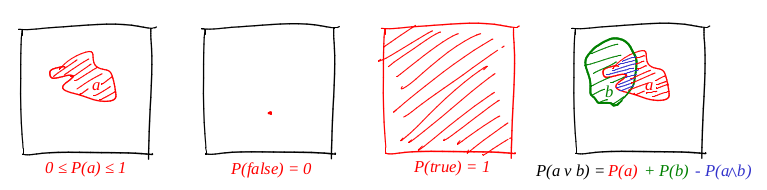
\includegraphics[width=.8\columnwidth]{axiomes.png}
\caption{A graphical illustration for the Kolmogorov's axioms}
\label{fig:kolmogorov}
\end{figure}

In 1931, de Finetti proved a very strong proposition:

\vspace{4mm}

\textit{If a bookmaker is guided by beliefs which break the axioms of the theory of probability,
then there exists such a combination of bets of the player which guarantees the loss for the bookmaker (a prize for the player) at each bet.
}

\vspace{4mm}

Probability axioms can be considered as the limiting set of probabilistic beliefs that some agent can adhere to.
Note that if a bookmaker respects Kolmogorov's axioms, it does not imply that he will win (leaving aside the fees),
however, if he does not respect the axioms, he is guaranteed to lose.
Other arguments have been put forward in favour of the probability theory;
but it is the practical success of probability-based reasoning systems that has proved to be very attractive.

To conclude the digression, it seems reasonable to base our reasoning on the probability theory.
Now let us proceed to maximum likelihood estimation, thus motivating the least squares.

\chapter{Maximum likelihood through examples}
\section{First example: coin toss}
\label{sec:cointoss}
Let us consider a simple example of coin flipping, also known as the Bernoulli's scheme. 
We conduct $n$ experiments, two events can happen in each one (``success'' or ``failure''): 
one happens with probability $p$, the other one with probability $1-p$. 
Our goal is to find the probability of getting exactly $k$ successes in these $n$ experiments. 
This probability is given by the Bernoulli's formula:
$$
P(k;n,p) = C_n^k p^k (1-p)^{n-k}
$$

Let us take an ordinary coin ($p=1/2$), flip it ten times ($n=10$), and count how many times we get the tails:
$$P(k) = C_{10}^k \frac{1}{2^k}\left(1-\frac{1}{2}\right)^{10-k} = \frac{C_{10}^k}{2^{10}}$$
Figure~\ref{fig:binomial}, left shows what a probability density graph looks like.

\begin{figure}[htb!]
\centering
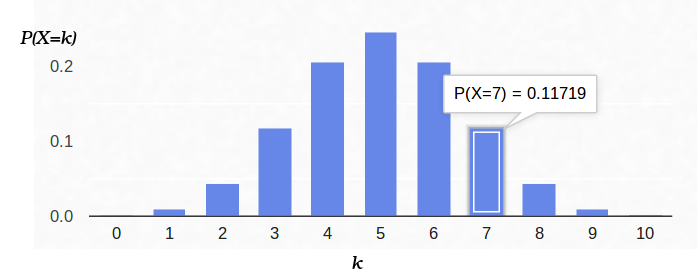
\includegraphics[width=.48\columnwidth]{binomial-05.png}
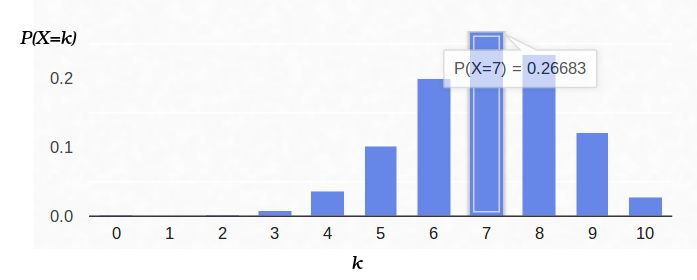
\includegraphics[width=.48\columnwidth]{binomial-07.png}
\caption{\textbf{Left:} probability density graph for the Bernoulli's scheme with $p=1/2$. \textbf{Right:} probability density graph for the Bernoulli's scheme with $p=7/10$.}
\label{fig:binomial}
\end{figure}

Thus, if we have fixed the probability of ``success'' ($1/2$) and also fixed the number of experiments (10), 
then the possible number of ``successes'' can be any integer between 0 and 10, but these outcomes are not equiprobable. 
It is clear that five ``successes'' are much more likely to happen than none. For example, the probability encountering seven tails is about 12\%.

Now let us look at the same problem from a different angle. 
Suppose we have a real coin, but we do not know its distribution of a priori probability of ``success''/``failure''. 
However, we can toss it ten times and count the number of ``successes''. 
For example, we have counted seven tails.
Would it help us to evaluate $p$?

We can try to fix $n=10$ and $k=7$ in the Bernoulli's formula, leaving $p$ as a free parameter:
$$\mathcal{L}(p) = C_{10}^7 p^7 (1-p)^3$$

Then the Bernoulli's formula can be interpreted as the plausibility of the parameter being evaluated (in this case $p$).
I have even changed the function notation, now it is denoted as $\mathcal L$ (likelihood).
That is being said, the likelihood is the probability to generate the observation data (7 tails out of 10 experiments) for the given value of the parameter(s).
For example, the likelihood of a balanced coin ($p=1/2$) with seven tails out of ten tosses is approximately 12\%. 
Figure~\ref{fig:likelihood} plots the likelihood function for the observation data with 7 tails out of 10 experiments.

\begin{figure}[htb!]
\centering
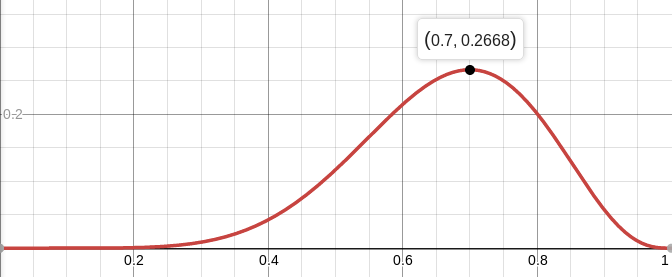
\includegraphics[width=.5\columnwidth]{likehood-07.png}
\caption{The plot of the likelihood function $\mathcal{L}(p)$ for the observation data with 7 tails out of 10 experiments.}
\label{fig:likelihood}
\end{figure}

So, we are looking for the parameter value that maximizes the likelihood of producing the observations we have.
In our particular case, we have a function of one variable, and we are looking for its maximum.
In order to make things easier, I will not search for the maximum of $\mathcal L$, but for the maximum of $\log \mathcal L$.
The logarithm is a strictly monotonous function, so maximizing both is equivalent.
The logarithm has a nice property of breaking down products into sums that are much more convenient to differentiate.
So, we are looking for the maximum of this function:
$$\log \mathcal{L}(p) = \log C_{10}^7 + 7 \log p + 3\log (1-p)$$

That's why we equate it's derivative to zero:
$$\frac{d \log \mathcal{L}}{dp} = 0$$

The derivative of $\log x = \frac{1}{x}$, therefore:
$$\frac{d \log \mathcal{L}}{dp} = \frac{7}{p} - \frac{3}{1-p} = 0$$

That is, the maximum likelihood (about 27\%) is reached at the point $p=7/10$.
Just in case, let us check the second derivative:
$$\frac{d^2 \log \mathcal{L}}{dp^2} = -\frac{7}{p^2} - \frac{3}{(1-p)^2}$$

In the point $p=7/10$ it is negative, therefore this point is indeed a maximum of the function $\mathcal{L}$:
$$\frac{d^2 \log \mathcal{L}}{dp^2}(0.7)  \approx -48 < 0$$

Figure~\ref{fig:binomial} shows the probability density graph for the Bernoulli's scheme with $p=7/10$.


\section{Second example: analog-to-digital converter (ADC)}

Let us imagine that we have a constant physical quantity that we want to measure; for example, it can be a length to measure with a ruler or a voltage with a voltmeter.
In the real world, any measurement gives \textit{an approximation} of this value, but not the value itself.
The methods I am describing here were developed by Gauß at the end of the 18th century, when he measured the orbits of celestial bodies
\footnote{Note that Legendre has published an equivalent method in 1805, 
whereas Gauß' first publication is dated by 1809. Gauß has always claimed that he had been using the method since 1795,
% https://projecteuclid.org/download/pdf_1/euclid.aos/1176345451
and this is a very famous priority dispute~\cite{stigler1981} in the history of statistics.
There are, however, numerous evidence to support the thesis that Gauß possessed the method before Legendre, but he was late in his communication.}.
%Theoria Motus Corporum Coelestium
~\cite{gauss1809theoria}

For example, if we measure the battery voltage $N$ times, we get $N$ different measurements. Which of them should we take? All of them! 
So, let us say that we have $N$ measurements $U_j$:
$$
\{U_j\}_{j=1}^{N}
$$

Let us suppose that each measurement $U_j$ is equal to the real value plus the Gaussian noise. 
The noise is characterized by two parameters --- the center of the Gaussian bell and its ``width''. 
In this case, the probability density can be expressed as follows:
$$
p(U_j) = \frac{1}{\sqrt{2\pi}\sigma} \exp\left(-\frac{(U_j-U)^2}{2\sigma^2}\right)
$$

That is, having $N$ measurements $U_j$, our goal is to find the parameters $U$ and $\sigma$ that maximize the likelihood.
The likelihood (I have already applied the logarithm) can be written as follows:
\begin{align*}
\log \mathcal{L}(U,\sigma) & = \log \left(\prod\limits_{j=1}^N  \frac{1}{\sqrt{2\pi}\sigma} \exp\left(-\frac{(U_j-U)^2}{2\sigma^2}\right)\right) =\\
& = \sum\limits_{j=1}^N \log \left(\frac{1}{\sqrt{2\pi}\sigma} \exp\left(-\frac{(U_j-U)^2}{2\sigma^2}\right)\right) = \\
& = \sum\limits_{j=1}^N \left(\log \left(\frac{1}{\sqrt{2\pi}\sigma}\right) -\frac{(U_j-U)^2}{2\sigma^2}\right) = \\
& = -N \left(\log\sqrt{2\pi} + \log\sigma\right) - \frac{1}{2\sigma^2} \sum\limits_{j=1}^N (U_j-U)^2
\end{align*}

And then everything is strictly as it used to be, we equate the partial derivatives to zero:
$$
\frac{\partial\log\mathcal{L}}{\partial U}    =  \frac{1}{\sigma^2}\sum\limits_{j=1}^N (U_j-U) = 0 
$$

The most plausible estimation of the unknown value $U$ is the simple average of all measurements:
$$
U = \frac{\sum\limits_{j=1}^N U_j}{N}
$$

And the most plausible estimation of $\sigma$ turns out to be the standard deviation:
$$
\frac{\partial\log\mathcal{L}}{\partial\sigma} =  -\frac{N}{\sigma} + \frac{1}{\sigma^3}\sum\limits_{j=1}^N (U_j-U)^2 = 0
$$

$$
\sigma = \sqrt{\frac{\sum\limits_{j=1}^N (U_j-U)^2}{N}} 
$$

Such a convoluted way to obtain a simple average of all measurements\dots
In my humble opinion, the result is worth the effort.
By the way, averaging multiple measurements of a constant value in order to increase the accuracy of measurements is quite a standard practice.
For example, ADC averaging. Note that the hypothesis of Gaussian noise is not necessary in this case, it is enough to have an unbiased noise.


\section{Third exampe, still 1D}

Let us re-consider the previous example with a small modification.
Let us say that we want to measure the resistance of a resistor.
We have a bench top power supply with current regulation.
That is, we control the current flowing through the resistance and we can measure the voltage required for this current.
So, our ``ohmmeter'' evaluates the resistance through $N$ meausrements $U_j$ for each reference current $I_j$:
$$
\{I_j, U_j\}_{j=1}^{N}
$$

If we draw these points on a chart (Figure~\ref{fig:URI}), the Ohm's law tells us that we are looking for the slope of the blue line that approximates the measurements.
\begin{figure}[htb!]
\centering
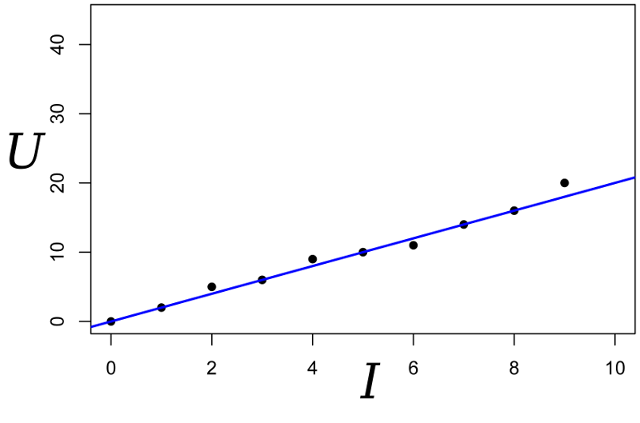
\includegraphics[width=.5\columnwidth]{URI.png}
\caption{Having $N$ meausrements $U_j$ for each reference current $I_j$, we are looking for the slope of the blue line that approximates the measurements through the Ohm's law.}
\label{fig:URI}
\end{figure}


Let us write the expression of the (logarithm of) likelihood of the parameters:
\begin{align*}
\log \mathcal{L}(R,\sigma) & = \log \left(\prod\limits_{j=1}^N  \frac{1}{\sqrt{2\pi}\sigma} \exp\left(-\frac{(U_j-R I_j)^2}{2\sigma^2}\right)\right) =\\
& = -N \left(\log\sqrt{2\pi} + \log\sigma\right) - \frac{1}{2\sigma^2} \sum\limits_{j=1}^N (U_j- R I_j)^2
\end{align*}

As usual, we equate the partial derivatives to zero:
\begin{align*}
\frac{\partial\log\mathcal{L}}{\partial R} &=  -\frac{1}{2\sigma^2}\sum\limits_{j=1}^N -2I_j (U_j- R I_j) = \\
&= \frac{1}{\sigma^2}\left(\sum\limits_{j=1}^N I_jU_j - R\sum\limits_{j=1}^N I_j^2\right) = 0
\end{align*}

Then the most plausible resistance $R$ can be found with the following formula:
$$
R = \frac{\sum\limits_{j=1}^N I_jU_j}{\sum\limits_{j=1}^N I_j^2}
$$

This result is somewhat less obvious than the simple average of all measurements in the previous example.
Note that if we take one hundred measurements with $\approx 1A$ reference current and one measurement with $\approx 1kA$ reference current,
then the first hundred measurements would barely affect the result. Let's remember this fact, we will need it later.

\section{Fourth example: back to the least squares}
\label{sec:springscale}
You have probably already noticed that in the last two examples, maximizing the logarithm of the likelihood is equivalent to minimizing the sum of squared estimation errors.
Let us consider one more example.
Say we want to calibrate a spring scale with a help of reference weights.
Suppose we have $N$ reference weights of mass $x_j$; we weigh them with the scale and measure the length of the spring.
So, we have $N$ spring lengths $y_j$:
$$
\{x_j, y_j\}_{j=1}^{N}
$$

Hooke's law tells us that spring stretches linearly on the force applied;
this force includes the reference weight and the weight of the spring itself. 
Let us denote the spring stiffness as $a$, and the spring length streched under under its own weight as $b$. 
Then we can express the plausibility of our measurements (still under the Gaussian measurement noise hypothesis) in this way:
\begin{align*}
\log \mathcal{L}(a, b,\sigma) & = \log \left(\prod\limits_{j=1}^N  \frac{1}{\sqrt{2\pi}\sigma} \exp\left(-\frac{(y_j - a x_j - b)^2}{2\sigma^2}\right)\right) =\\
& = -N \left(\log\sqrt{2\pi} + \log\sigma\right) - \frac{1}{2\sigma^2} \sum\limits_{j=1}^N (y_j- a x_j - b)^2
\end{align*}

Maximizing the likelihood of $\mathcal L$ is equivalent to minimizing the sum of the squared estimation error, i.e., we are looking for the minimum of the function $S$ defined as follows:
$$
S(a, b) = \sum\limits_{j=1}^N (y_j- a x_j - b)^2
$$


\begin{figure}[htb!]
\centering
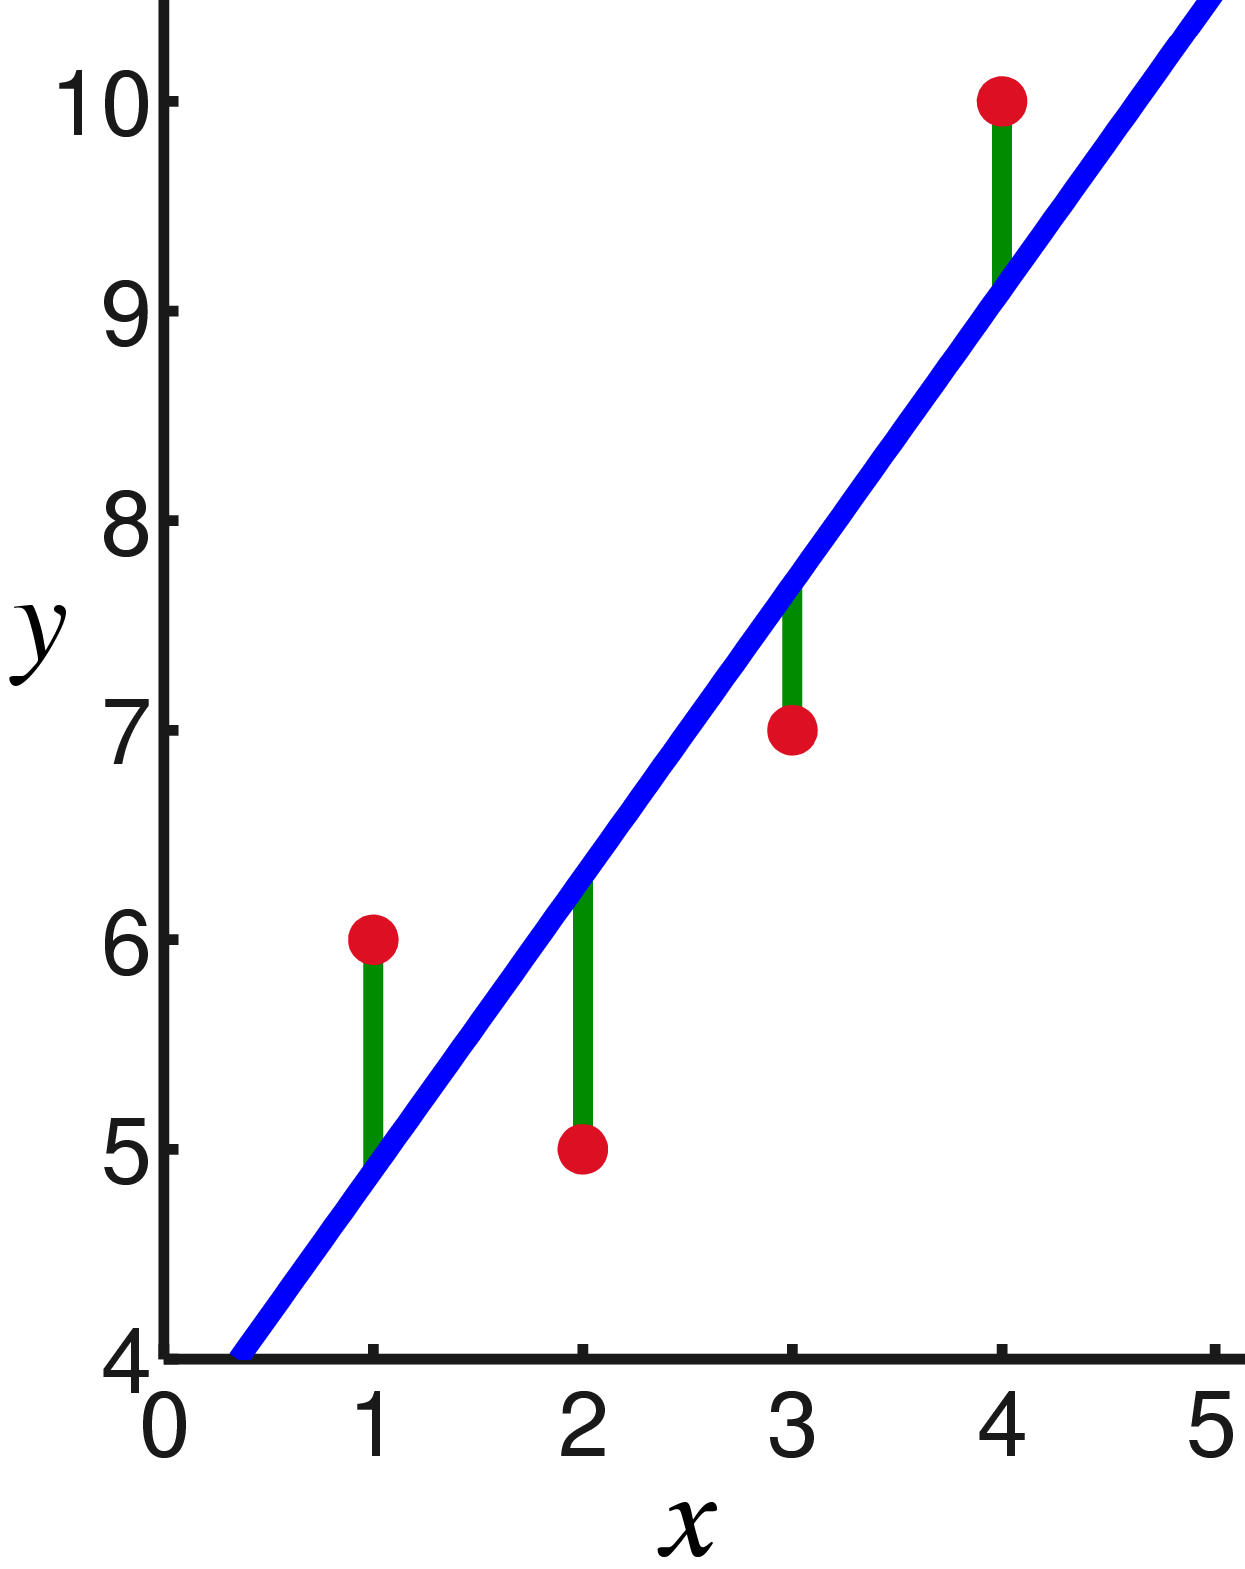
\includegraphics[width=.2\columnwidth]{c5aa80f6a2e9575abfa7b3dfdabf5c5a.png}
\caption{To calibrate the spring scale, we can solve the linear regression problem.}
\label{fig:regression}
\end{figure}

Figure~\ref{fig:regression} illustrates the formula: we are looking for such a straight line that minimizes the sum of squared lengths of green segments.
And then the derivation is quite straightforward:
\begin{align*}
\frac{\partial S}{\partial a} &= \sum\limits_{j=1}^N 2 x_j (a x_j + b - y_j) = 0 \\
\frac{\partial S}{\partial b} &= \sum\limits_{j=1}^N 2 (a x_j + b - y_j) = 0
\end{align*}

We obtain a system of two linear equations with two unknowns:
$$
\left \{ \begin{array}{r l}
a \sum\limits_{j=1}^N x_j^2 + b \sum\limits_{j=1}^N x_j  & = \sum\limits_{j=1}^N x_j y_j\\
a \sum\limits_{j=1}^N x_j   + b N                        & = \sum\limits_{j=1}^N y_j
\end{array} \right.
$$

Use your favorite method to obtain the following solution:
\begin{align*}
a &= \frac{N \sum\limits_{j=1}^N x_j y_j - \sum\limits_{j=1}^N x_j \sum\limits_{j=1}^N y_j}{N\sum\limits_{j=1}^N x_j^2 - \left(\sum\limits_{j=1}^N x_j\right)^2} \\
b &= \frac{1}{N}\left(  \sum\limits_{j=1}^N y_j - a  \sum\limits_{j=1}^N x_j \right)
\end{align*}

\section*{Conclusion}
The least squares method is a particular case of maximizing likelihood in cases where the probability density is Gaussian.
If the density is not Gaussian, the least squares approach can produce an estimate different from the MLE (maximum likelihood estimation).
By the way, Gauß conjectured that the type of noise is of no importance, and the only thing that matters is the independence of trials.

As you have already noticed, the more we parameters we have, the more cumbersome the analytical solutions are.
Fortunately, we are not living in XVIII century anymore, we have computers!
Next we will try to build a geometric intuition on least squares, and see how can least squares problems be efficiently implemented.


\authoredby{B}
\chapter{Introduction to systems of linear equations}
\fancyhead[R]{\textcolor{ao(english)}{core text}}
\label{ch:linsyst}

\section{Smooth an array}
\label{sec:arraysmooth}
The time has come to write some code. Let us examine the following program:
\inputminted[frame=single,linenos=true]{python}{listings/example_3.1.py}
We start from a 16 elements array, and we iterate over and over a simple procedure: we replace each element with a barycenter of its neighbours;
the first and the last element are fixed. What should we get at the end? Does it converge or would it oscillate infinitely?
Intuitively, each peak in the signal is cut out, and therefore the array will be smoothed over time.
Top left image of the Figure~\ref{fig:linsys_smooth} shows the initialization of the array \mintinline{python}{x},
other images show the evolution of the data.

\begin{figure}[ht]
    \centering
    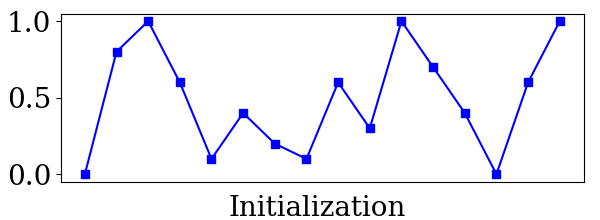
\includegraphics[width=.32\linewidth]{example_3.1_0.png}
    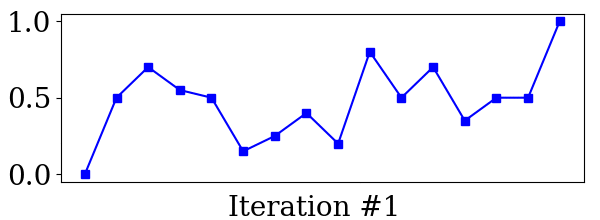
\includegraphics[width=.32\linewidth]{example_3.1_1.png}
    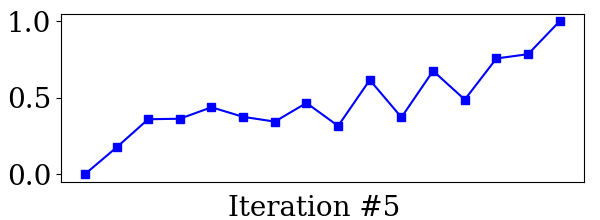
\includegraphics[width=.32\linewidth]{example_3.1_2.png}
    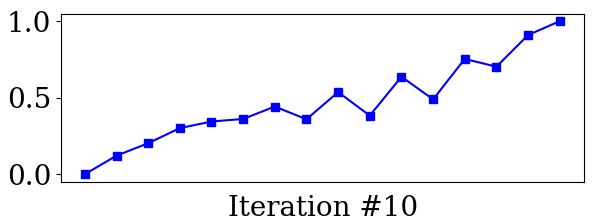
\includegraphics[width=.32\linewidth]{example_3.1_3.png}
    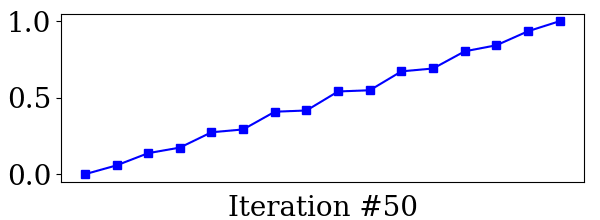
\includegraphics[width=.32\linewidth]{example_3.1_4.png}
    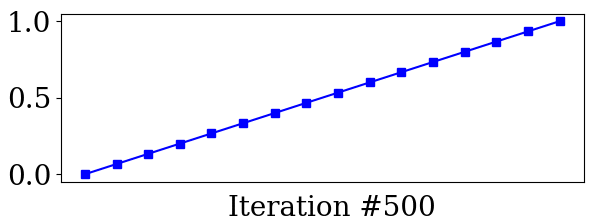
\includegraphics[width=.32\linewidth]{example_3.1_5.png}
\caption{Smoothing an array: first 500 iterations of the program from \S~\ref{sec:arraysmooth}.}
    \label{fig:linsys_smooth}
\end{figure}

Is there a way to predict the result without guessing or executing the program? The answer is yes; but first let us recall how to solve systems of linear equations.

\section{The Jacobi and Gauß-Seidel iterative methods}
\label{sec:gauss-seidel}
Let us suppose that we have an ordinary system of linear equations:
$$
\left\{
\begin{array}{cccccccc}
a_{11}x_1 & + &  a_{12}x_2  &+      & \cdots & + & a_{1n}x_n &= b_1\\
a_{21}x_1 & + &  a_{22}x_2  &+      & \cdots & + & a_{2n}x_n &= b_2\\
          &   &             &\vdots &        &   &           &     \\
a_{n1}x_1 & + &  a_{n2}x_2  &+      & \cdots & + & a_{nn}x_n &= b_n\\
\end{array}
\right.
$$
It can be rewritten by leaving  $x_i$ only on the left side of the equations:
\begin{align*}
x_1 &= \frac{1}{a_{11}}(b_1 - a_{12}x_2 - a_{13}x_3 - \cdots - a_{1n}x_n)\\
x_2 &= \frac{1}{a_{22}}(b_2 - a_{21}x_1 - a_{23}x_3 - \cdots - a_{2n}x_n)\\
    & \qquad \vdots \\
x_n &= \frac{1}{a_{nn}}(b_n - a_{n1}x_1 - a_{n2}x_2 - \cdots - a_{n,n-1}x_{n-1})
\end{align*}

Suppose that we have an arbitrary vector $\vec{x}^{(0)}=\left(x_1^{(0)}, x_2^{(0)}, \dots, x_n^{(0)}\right)$, approximating the solution (an initial guess, for example, a zero vector).
Then, if we plug it into the right side of the equations, we can compute an updated approximated solution $\vec{x}^{(1)}=\left(x_1^{(1)}, x_2^{(1)}, \dots, x_n^{(1)}\right)$.
In other words, $\vec{x}^{(1)}$ is derived from $\vec{x}^{(0)}$ as follows:
\begin{align*}
x_1^{(1)} &= \frac{1}{a_{11}}(b_1 - a_{12}x_2^{(0)} - a_{13}x_3^{(0)} - \cdots - a_{1n}x_n^{(0)})\\
x_2^{(1)} &= \frac{1}{a_{22}}(b_2 - a_{21}x_1^{(0)} - a_{23}x_3^{(0)} - \cdots - a_{2n}x_n^{(0)})\\
    & \qquad \vdots \\
x_n^{(1)} &= \frac{1}{a_{nn}}(b_n - a_{n1}x_1^{(0)} - a_{n2}x_2^{(0)} - \cdots - a_{n,n-1}x_{n-1}^{(0)})
\end{align*}

Repeating the process $k$ times, the solution can be approximated by the vector $\vec{x}^{(k)}=\left(x_1^{(k)}, x_2^{(k)}, \dots, x_n^{(k)}\right)$.
Let us write down the recursive formula just in case:
$$
x_i^{(k)} = \frac{1}{a_{ii}} \left(b_i - \sum\limits_{j=1,j\neq i}^n a_{ij}x_j^{(k-1)} \right), \quad \text{for } i=1,2,\dots,n
$$

Under some assumptions about the system (for example, it is quite obvious that diagonal elements must not be zero), this procedure converges to the true solution.
This iteration is known as the Jacobi method.
Of course, there are other much more powerful numeric methods, for example, the conjugate gradient method, but the Jacobi method is the simplest one.

What is the connection with the code from \S\ref{sec:arraysmooth}? It turns out that the program solves the following system with the Jacobi method:
\begin{equation}
\label{eq:1d:smooth}
\left\{
\begin{array}{rl}
 x_0 &= 0 \\
x_1-x_0 &= x_2-x_1 \\
x_2-x_1 &= x_3-x_1 \\
     &  \vdots \\
x_{13}-x_{12}     &= x_{14}-x_{13} \\
x_{14}-x_{13}     &= x_{15}-x_{14} \\
x_{15} &= 1 \\
\end{array}
\right.
\end{equation}
Do not take my word for it, grab a pencil and verify it!
So, if we consider the array as a sampled function, the linear system prescribes a constant derivative and fixes the extremities, therefore the result can only be a straight line.

There is a very interesting modification of the Jacobi method, named after Johann Carl Friedrich Gauß and Philipp Ludwig von Seidel.
This modification is even easier to implement than the Jacobi method, and it often requires fewer iterations to produce the same degree of accuracy.
With the Jacobi method, the values of obtained in the $k$-th approximation remain unchanged until the entire
$k$-th approximation has been calculated. With the Gauß-Seidel method, on the other hand, we use the new values of each as soon as they are known.
The recursive formula can be written as follows:
$$
x_i^{(k)} = \frac{1}{a_{ii}} \left(b_i - \sum\limits_{j=1}^{i-1} a_{ij}x_j^{(k)} -  \sum\limits_{j=i+1}^n a_{ij}x_j^{(k-1)} \right), \quad \text{for } i=1,2,\dots,n
$$

It allows to perform all the computations in place. The following program solves the same equation~\eqref{eq:1d:smooth} by the Gauß-Seidel method:
\inputminted[frame=single,linenos=true]{python}{listings/example_3.2.py}
Figure~\ref{fig:arraysmooth_gs} shows the behaviour of this program.

\begin{figure}[ht]
    \centering
    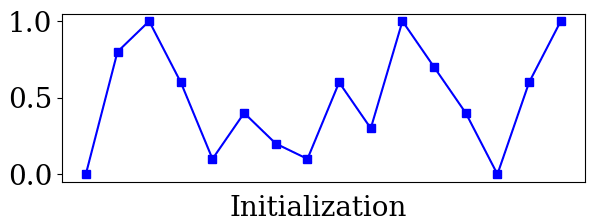
\includegraphics[width=.32\linewidth]{example_3.2_0.png}
    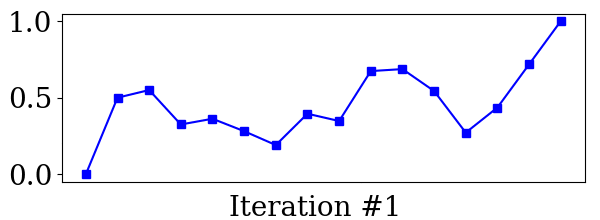
\includegraphics[width=.32\linewidth]{example_3.2_1.png}
    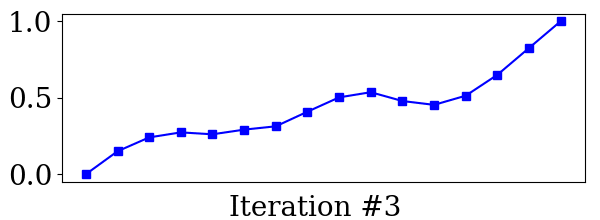
\includegraphics[width=.32\linewidth]{example_3.2_2.png}
    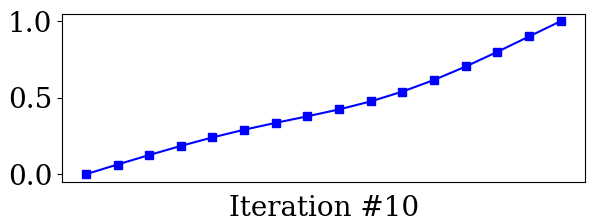
\includegraphics[width=.32\linewidth]{example_3.2_3.png}
    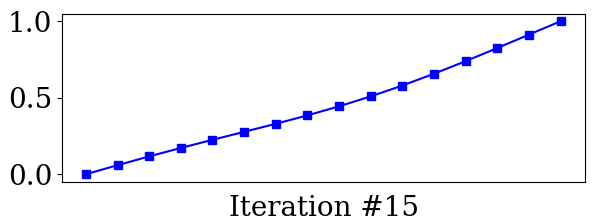
\includegraphics[width=.32\linewidth]{example_3.2_4.png}
    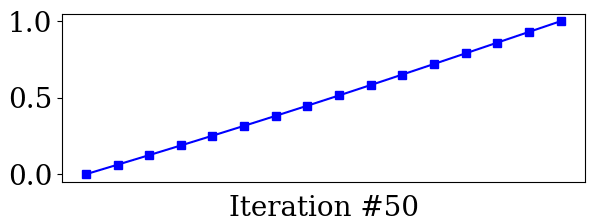
\includegraphics[width=.32\linewidth]{example_3.2_5.png}
    \caption{Linear function via Gauß-Seidel iteration (\S\ref{sec:gauss-seidel}).}
    \label{fig:arraysmooth_gs}
\end{figure}

\section{Smoothing a 3D surface}
\label{sec:3dsmooth}
There is no much fun in studying small 1D arrays, let us play with a triangulated surface! The following listing is a direct equivalent of the previous one:
\inputminted[frame=single,linenos=true]{cpp}{listings/example_3.3.cpp}
All boundary vertices are fixed, and all the interiour vertices are iteratively placed in the barycenter of their immediate neighbors.
Can you predict the result?

First of all, let us see that the system \eqref{eq:1d:smooth} can be rewritten as follows:
\begin{equation}
\label{eq:1d:smooth-laplacian}
\left\{
\begin{array}{cccccccccccl}
 x_0 &       &       &       &      &        &         &          &          &          &         &= 0 \\
-x_0 & +2x_1 & -x_2  &       &      &        &         &          &          &          &         &= 0 \\
     & -x_1  & +2x_2 & -x_3  &      &        &         &          &          &          &         &= 0 \\
     &       & -x_2  & +2x_3 & -x_4 &        &         &          &          &          &         &= 0 \\
     &       &       &       &      & \ddots &         &          &          &          &         &  \vdots \\
     &       &       &       &      &        & -x_{11} & +2x_{12} & -x_{13}  &          &         &= 0 \\
     &       &       &       &      &        &         & -x_{12}  & +2x_{13} & -x_{14}  &         &= 0 \\
     &       &       &       &      &        &         &          & -x_{13}  & +2x_{14} & -x_{15} &= 0 \\
     &       &       &       &      &        &         &          &          &          &  x_{15} &= 1 \\
\end{array}
\right.
\end{equation}
You can see the pattern for the second-order finite difference.
Computing a constant derivative function is equivalent to computing a function with zero second derivative, it is only logic that the result is a straight line.

It is all the same for our 3D surface, the above code solves the Laplace's equation $\Delta f = 0$ with Dirichlet boundary conditions.
Again, do not trust me, grab a pencil and write down the corresponding matrix for a mesh with one interior vertex.
So, the result must be the minimal surface respecting the boundary conditions.
In other words, make a loop from a rigid wire, soak it in a liqud soap, the soap film on this loop is the solution.
Figure~\ref{fig:minsurface} provides an illutration.
\begin{figure}[ht]
    \centering
    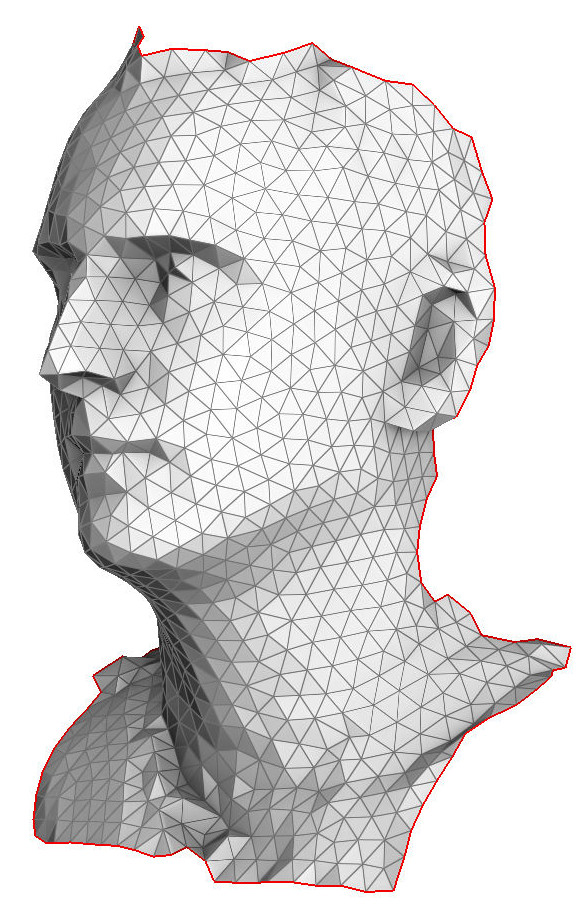
\includegraphics[width=.2\linewidth]{example_3.3_0.jpg}
    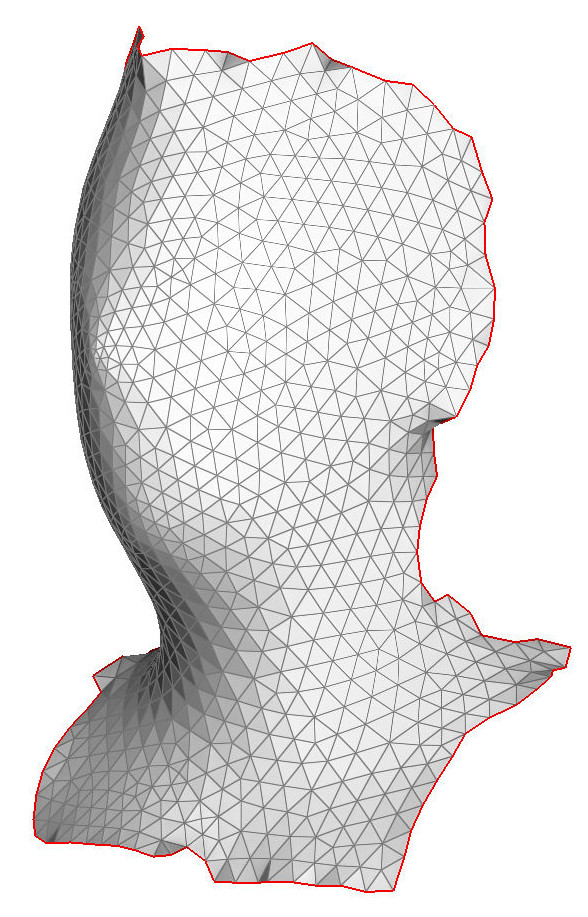
\includegraphics[width=.2\linewidth]{example_3.3_1.jpg}
    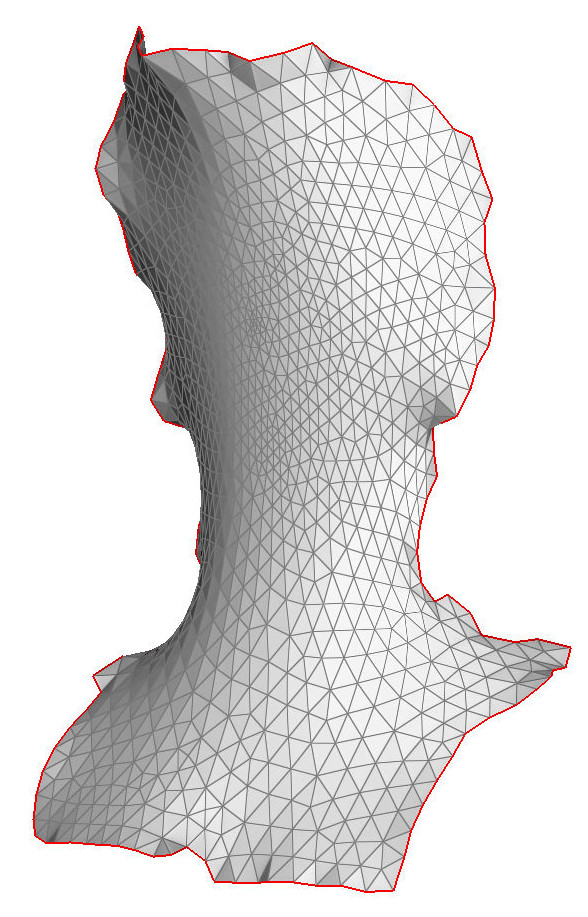
\includegraphics[width=.2\linewidth]{example_3.3_2.jpg}
    \caption{Smoothing a 3D surface (\S\ref{sec:3dsmooth}). \textbf{Left:} the input surface; \textbf{middle:} 10 iterations; \textbf{right:} 1000 iterations.}
    \label{fig:minsurface}
\end{figure}



\section{Prescribe the right hand side}
\label{sec:rhs}

Let us return to the equation~\eqref{eq:1d:smooth-laplacian}, but this time the right hand side would not be zero:
\inputminted[frame=single,linenos=true]{python}{listings/example_3.4.py}
What is the result of this program? Well, it is easy to answer. We are looking for a function whose second derivative is a linear function,
therefore the solution must be a cubic polynomial. Figure~\ref{fig:linsys-cubic} shows the evolution of the array, the ground truth polynomial is shown in green.

\begin{figure}[ht]
    \centering
    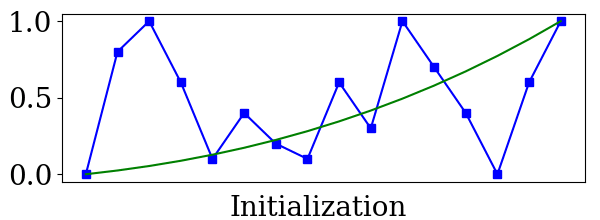
\includegraphics[width=.32\linewidth]{example_3.4_0.png}
    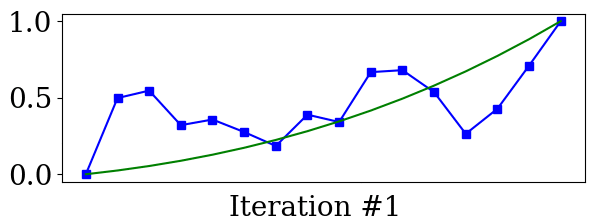
\includegraphics[width=.32\linewidth]{example_3.4_1.png}
    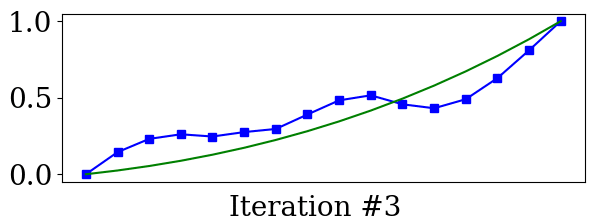
\includegraphics[width=.32\linewidth]{example_3.4_2.png}
    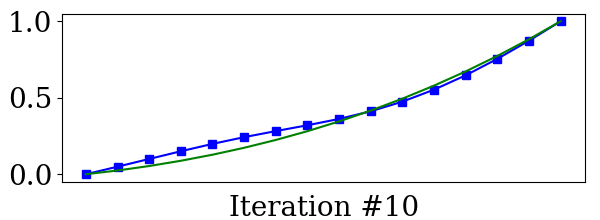
\includegraphics[width=.32\linewidth]{example_3.4_3.png}
    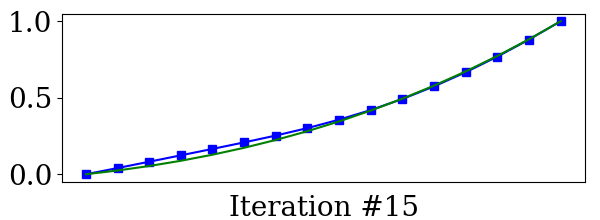
\includegraphics[width=.32\linewidth]{example_3.4_4.png}
    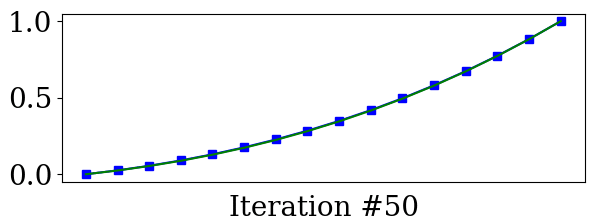
\includegraphics[width=.32\linewidth]{example_3.4_5.png}
    \caption{Reconstructing a cubic function (\S\ref{sec:rhs}); the ground truth is shown in green.}
    \label{fig:linsys-cubic}
\end{figure}

Congratulations, you have just solved a Poisson's equation!

%\section{3D example}
%\begin{figure}[ht]
%	\centering
%	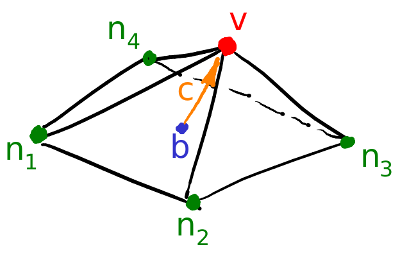
\includegraphics[width=.3\linewidth]{barycenter/1ring.png}
%	\caption{.}
%	\label{fig:????}
%\end{figure}

%\begin{figure}[ht]
%	\centering
%	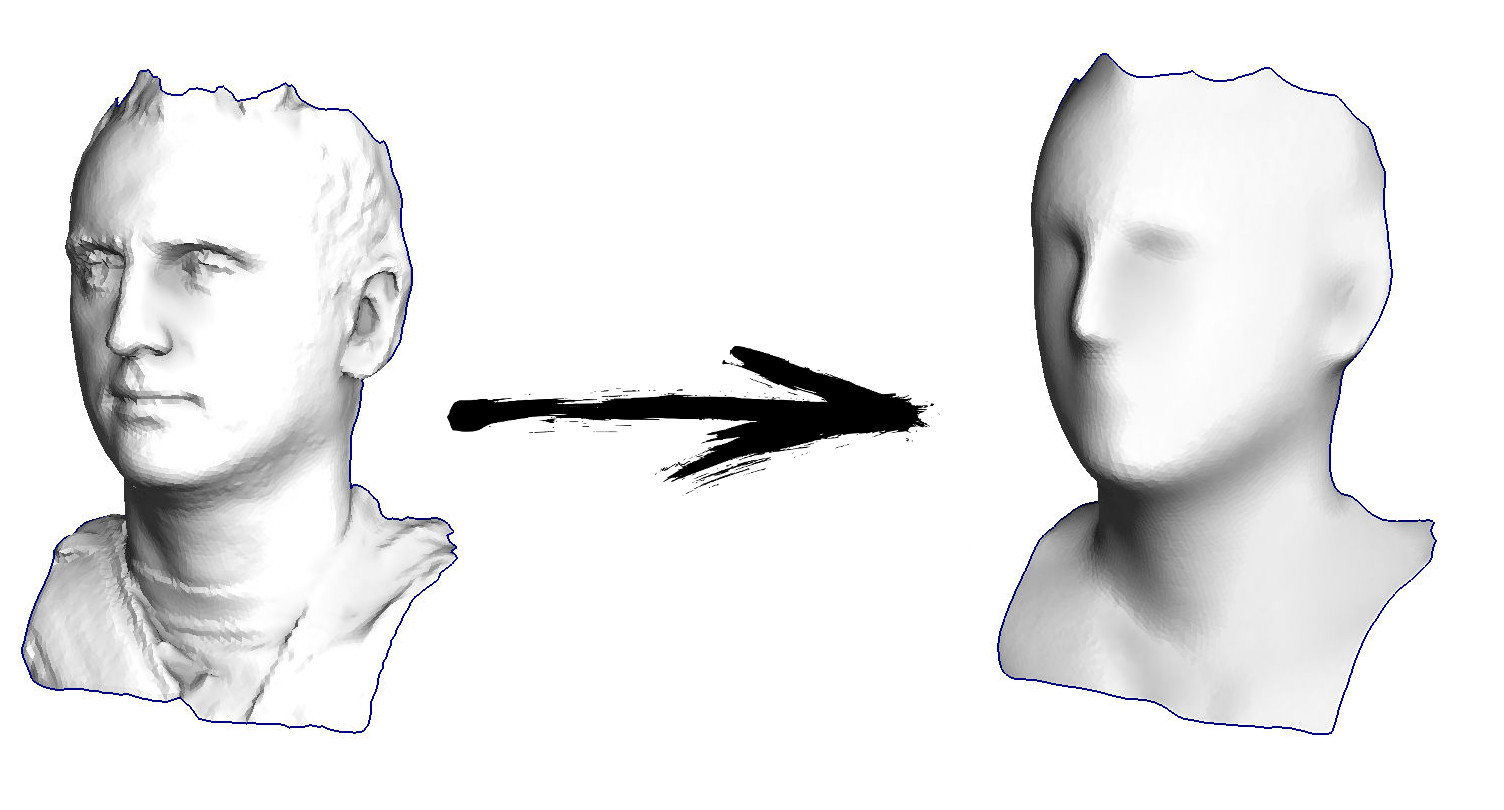
\includegraphics[width=.8\linewidth]{barycenter/ls-teaser2.jpg}
%	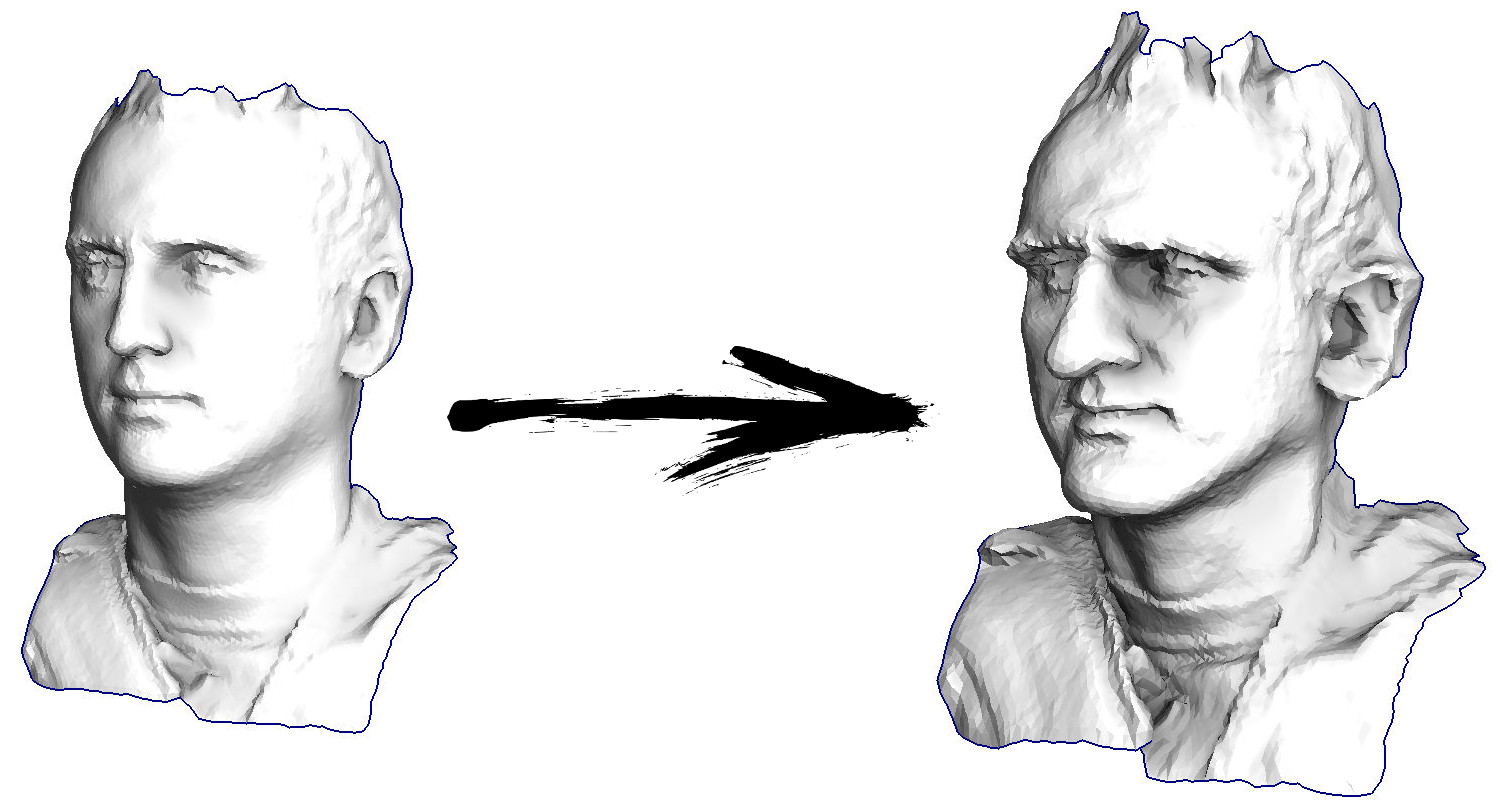
\includegraphics[width=.8\linewidth]{barycenter/ls-teaser.jpg}
%%	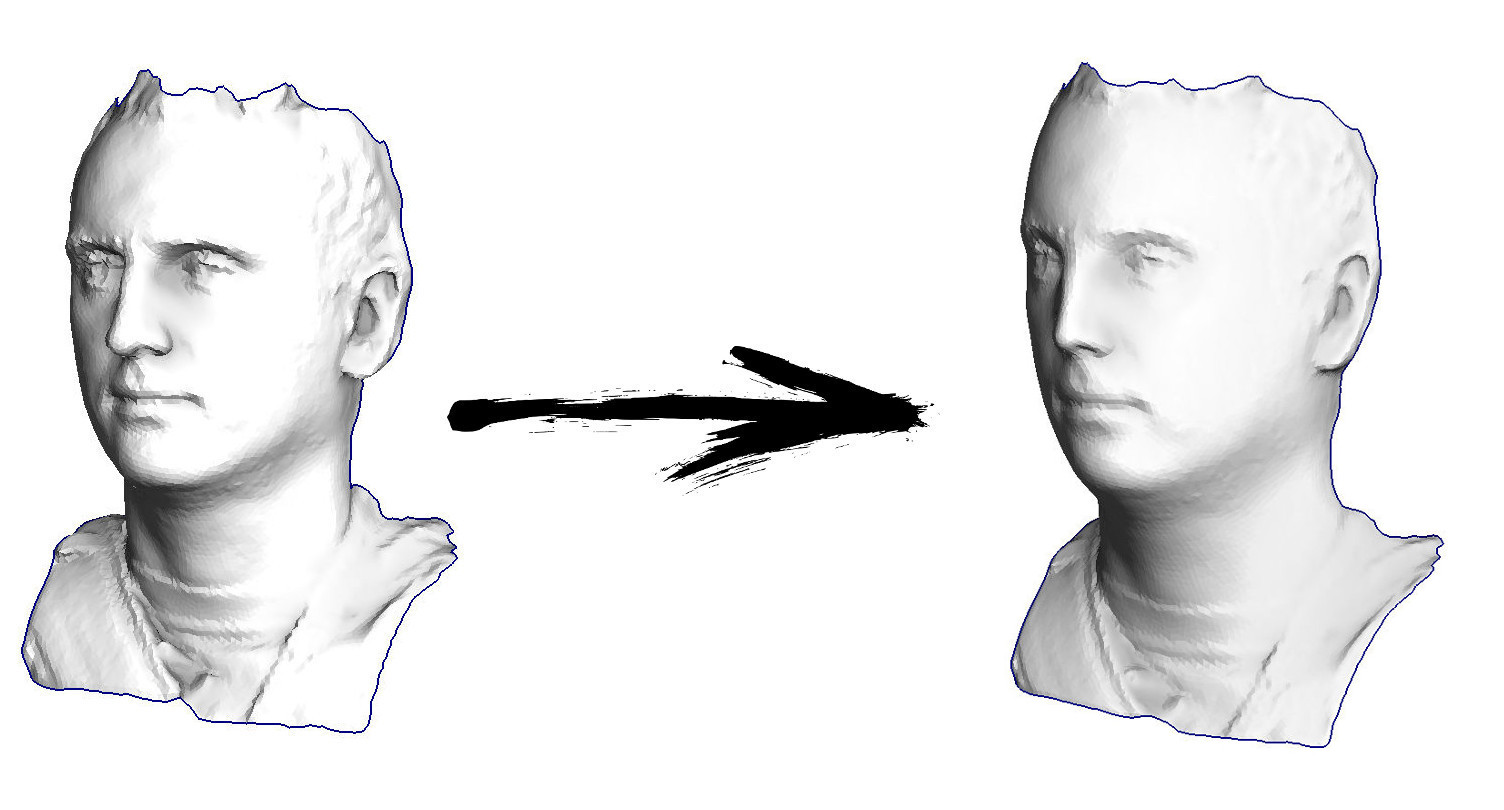
\includegraphics[width=.8\linewidth]{barycenter/ls-teaser3.jpg}
%	\caption{.}
%	\label{fig:????}
%\end{figure}


\authoredby{A}
\chapter{Finite elements example}
\fancyhead[R]{\textcolor{blue}{optional for reading}}

In the previous section we saw that mere 3 lines of code can be sufficient to solve a linear system, and this linear system corresponds to a differential equation.
While it is extremely cool, what are the practical consequences for a programmer?  How do we build these systems? Where do we use them?
Well, there is a huge community of people who start with a continuous problem, then the problem is carefully discretized and eventually reduced to a linear system.
In this chapter I show a tiny bit of the bottomless pit called finite element methods.
Namely, I show a mathematician's approach to the program we saw in \S\ref{sec:rhs}.
Note that this chapter is marked as \textcolor{blue}{optional}.
It is here to make connections to adjacent domains; feel free to skip it, the core text about least squares continues in the next chapter.

This chapter is closely related both to \S\ref{sec:rhs} and the chapter that follows.
In \S\ref{sec:equadiff} we introduce two fundamental methods for determining the coefficients of the linear system from \S\ref{sec:rhs}.
We start with an illustration on 2D vectors, because vectors in vector spaces give a more intuitive understanding than starting directly with approximation of functions in function spaces.

\section{Approximation of vectors}

Suppose we have given a vector $\vec{\varphi}$ and that we want to approximate this vector by a vector aligned with the vector $\vec{w}$.
Figure~\ref{fig:vector_approximation} vector depicts the situation.

\begin{figure}[ht]
	\centering
	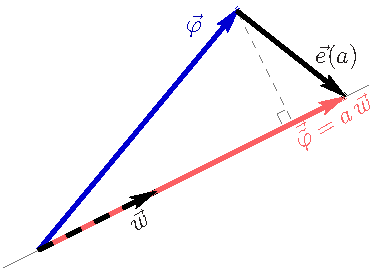
\includegraphics[width=.4\linewidth]{vector_approximation.pdf}
	\caption{Approximation of a vector $\vec{\varphi}$ by a vector $\vec{\tilde{\varphi}}$ constrained to be collinear with a chosen vector $\vec{w}$.}
	\label{fig:vector_approximation}
\end{figure}

Our aim is to find the vector $\vec{\tilde{\varphi}} = a\vec{w}$ which best approximates the given vector $\varphi$.
A reasonable criterion for the best approximation could be to minimize the length $\|\vec{e}(a)\|$ of the difference between the approximation $\tilde\varphi$ and the given $\varphi$.
Note that this norm is minimized when $\vec{e}(a) \perp \vec{w}$.

\section{Approximation of functions}
\label{sec:equadiff}

In this section we will consider a simple boundary value problem and its relation to systems of linear equations.
The boundary value problem is the problem of finding a solution to a given differential equation satisfying boundary conditions at the the boundary of a region.
Let us start with a ground truth function defined as 
$$
\varphi(x) := \frac{1}{6} x^3 + \frac{1}{2} x^2 + \frac{1}{3} x.
$$
This function is unknown, and we list it here to compare our solution to the ground truth.
Let us define a function $f(x) := x+1$.
It is simply the second derivative of $\varphi(x)$, but remember that $\varphi(x)$ is not known!
So, the problem is to find a function $\varphi(x)$ with prescribed second derivative and constrained at the limits of a region.
One possible instance of the boundary value problem can be written as follows:
\begin{equation}
\label{eq:femproblem}
\left\{
\begin{split}
\mathcal A\varphi(x) = f(x), \quad 0 < x < 1\\
\mathcal A=\frac{d^2}{dx^2}, \quad \varphi(0)=0, \quad \varphi(1)=1
\end{split}
\right.
\end{equation}
Here $f(x)$ is known, $\varphi(x)$ is unknown, but we have specified its values at the boundary.

In general, finite elements method searches for an \textit{approximated} solution of the problem.
The finite element method does not operate directly on the differential equations; instead the boundary problem is put into equivalent variational form.
The solution apperas in the integral over a quantity over the domain. The integral of a function over an arbitrary domain can be broken up into the sum of integrals over an arbitrary collection 
of subdomains called finite elements. As long as the subdomains are sufficiently small, polynomial functions can adequately represent the local behaviour of the solution.

Let us split the interval in $n$ parts, these subsegments are the \textit{elements}.
For example, for $n=3$ we can define four equispaced nodes $x_i$:
$$
x_0 := 0, \quad x_1 := \frac{1}{3}, \quad x_2 := \frac{2}{3}, \quad x_3 := 1.
$$
Note that equal distance is chosen here for the simplicity of presentation, and is not a requirement for the method.
Then a set of functions is to be defined over the elements; the approximated solution $\tilde{\varphi}$ is defined as a weighted sum of these functions.

For example, let us choose a set of piecewise linear functions (refer to Figure~\ref{fig:fem:blending} for an illustration):
$$
w_i(x) := \left\{
\begin{split}
\frac{x-x_{i-1}}{x_i-x_{i-1}}, & \quad x_{i-1}\leq x \leq x_i \\
\frac{x_{i+1}-x}{x_{i+1}-x_i}, & \quad x_i\leq x \leq x_{i+1}\\
0 & \quad \text{otherwise}
\end{split}
\right.
$$

\begin{figure}[ht]
\begin{minipage}{.45\linewidth}
	\centering
	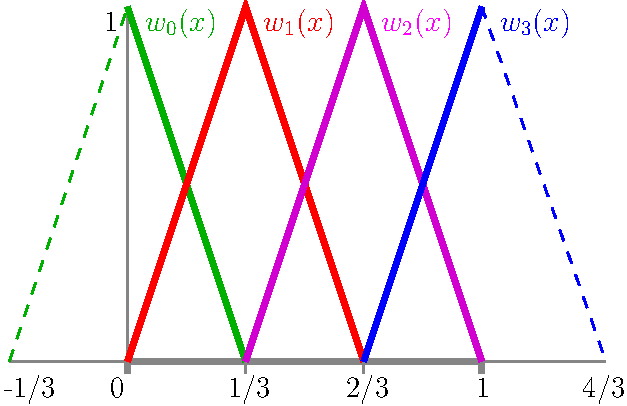
\includegraphics[width=\linewidth]{blending_functions.pdf}
	\caption{Hat function basis for FEM approximation.}
	\label{fig:fem:blending}
\end{minipage}
\hspace{.05\linewidth}
\begin{minipage}{.5\linewidth}
	\centering
	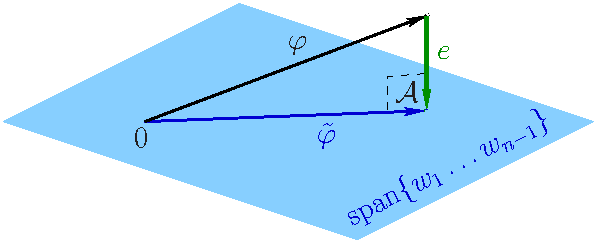
\includegraphics[width=\linewidth]{galerkin.pdf}
	\caption{The Galerkin method imposes $\mathcal A$-orthogonality between the solution space $\Span\{w_1,\dots w_{n-1}\}$ and the solution error  $e := \tilde{\varphi} - \varphi$.}
	\label{fig:galerkin}
\end{minipage}
\end{figure}

This choice is somewhat arbitrary, there are numerous possible bases.
Then the approximate solution is a linear combination of the weighting functions:
\begin{equation}
\label{eq:tildephi}
\tilde{\varphi}(x) := 0\cdot w_0(x) + b\cdot w_1(x) + c\cdot w_2(x) + 1\cdot w_3(x),
\end{equation}
where the coefficients of $w_0(x)$ and $w_3(x)$ are the direct consequence of the boundary condition $\varphi(0)=0$, $\varphi(1)=1$;
note that $b$ and $c$ give the values of the approximation for the points $x=\frac{1}{3}$ and $x=\frac{2}{3}$, respectively.
In the rest of the section we present two different ways to find the coefficients $b$ and $c$.

\subsection{The Galerkin method}
At first, let us try to use the classic Galerkin method for finding the approximate solution $\tilde \varphi$ of the problem~\eqref{eq:femproblem}.
Ideally, as we have done for vectors (Figure~\ref{fig:vector_approximation}), to approximate $\varphi$, we would like to project it onto the solution space $\Span\{w_1,\dots w_{n-1}\}$,
and thus to ask for the error $\tilde\varphi - \varphi$ to be orthogonal to $\Span\{w_1,\dots w_{n-1}\}$.
The problem, however, is that with a differential equation we do not know how to measure the true error ($\varphi$ is unknown).
Nevertheless, we can measure the residual $\mathcal A\tilde{\varphi} - f$ and we can project it onto $\Span\{w_1,\dots w_{n-1}\}$.
This corresponds to $\mathcal A$-orthogonality between the true error $\tilde\varphi - \varphi$ and the solution space, Figure~\ref{fig:galerkin} provides an illustration.

The residual being orthogonal to the solution space can be written as the following system of $n-1$ equations:
\begin{equation}
\label{eq:galerkin}
\int\limits_0^1 w_i \cdot \left(\mathcal A\tilde{\varphi} - f\right) dx = 0, \quad i = 1\dots n-1 
\end{equation}

Note that $w_i(x)$ is equal to zero outside the interval $[x_{i-1}, x_{i+1}]$, this allows us to rewrite the system:
$$
\int\limits_{x_{i-1}}^{x_{i+1}} w_i \cdot \frac{d^2\tilde{\varphi}}{dx^2}\,dx - \int\limits_{x_{i-1}}^{x_{i+1}} w_i\cdot f\,dx = 0, \quad i = 1\dots n-1
$$

Most often both integrals are evaluated numerically, or symbolic calculations are peformed over the left integral only.
The left integral is a dot product between the basis functions and the differential operator defined on a combination of basis functions;
it depends on the choice of the basis and can be precomputed.
As our problem is very simple, we will find the solution analytically.

Attention! The next step will be done on a slippery ground.
Our weighting functions are not differentiable everywhere, and caution must be taken.
Anyhow, let us integrate by parts the first integral:
\begin{align*}
\int\limits_{x_{i-1}}^{x_{i+1}} w_i \cdot \frac{d^2\tilde{\varphi}}{dx^2}\,dx &= 
\int\limits_{x_{i-1}}^{x_{i}} w_i \cdot \frac{d^2\tilde{\varphi}}{dx^2}\,dx + 
\int\limits_{x_{i}}^{x_{i+1}} w_i \cdot \frac{d^2\tilde{\varphi}}{dx^2}\,dx = \\
& =\underbrace{\lim\limits_{\varepsilon\rightarrow 0}w_i\cdot \frac{d\tilde{\varphi}}{dx}\Big|_{x_{i-1}+\varepsilon}^{x_{i}-\varepsilon} +
\lim\limits_{\varepsilon\rightarrow 0}w_i\cdot \frac{d\tilde{\varphi}}{dx}\Big|_{x_{i}+\varepsilon}^{x_{i+1}-\varepsilon}}_{= 0} - \int\limits_{x_{i-1}}^{x_{i+1}} \frac{dw_i}{dx}\cdot \frac{d\tilde{\varphi}}{dx}\,dx  = \\
& = - \int\limits_{x_{i-1}}^{x_{i+1}} \frac{dw_i}{dx}\cdot \frac{d\tilde{\varphi}}{dx}\,dx \\
\end{align*}

It allows us to rewrite the system~\eqref{eq:galerkin} as follows:
\begin{equation}
\label{eq:galerkin:system}
\int\limits_{x_{i-1}}^{x_{i+1}} \frac{dw_i}{dx} \cdot \frac{d\tilde{\varphi}}{dx}\,dx + \int\limits_{x_{i-1}}^{x_{i+1}} w_i\cdot f\,dx = 0, \quad i = 1\dots n-1
\end{equation}

In our particular example we have two equations ($n=3$), let us instantiate the functions:
$$
\frac{d\tilde{\varphi}}{dx} (x) := \left\{
\begin{split}
3b, & \quad 0 < x < \frac{1}{3}\\
-3b+3c, & \quad \frac{1}{3} < x < \frac{2}{3}\\
-3c+3, & \quad \frac{2}{3} < x < 1\\
0 & \quad \text{otherwise}
\end{split}
\right.
$$

$$
\frac{dw_1}{dx} (x) := \left\{
\begin{split}
3, & \quad 0 < x < \frac{1}{3}\\
-3, & \quad \frac{1}{3} < x < \frac{2}{3}\\
0 & \quad \text{otherwise}
\end{split}
\right.
$$

$$
\frac{dw_2}{dx} (x) := \left\{
\begin{split}
3, & \quad \frac{1}{3} < x < \frac{2}{3}\\
-3, & \quad \frac{2}{3} < x < 1\\
0 & \quad \text{otherwise}
\end{split}
\right.
$$

By plugging these instances into the system~\eqref{eq:galerkin:system} we can rewrite it as follows:
$$
\left\{
\begin{split}
\int\limits_{0}^{1/3} 3\cdot 3b\,dx + \int\limits_{1/3}^{2/3} -3\cdot (-3b+3c)\, dx + \int\limits_{0}^{1/3} 3x(x+1)\,dx + \int\limits_{1/3}^{2/3}(2-3x)(x+1)\,dx &= 0\\
\int\limits_{1/3}^{2/3} 3\cdot (-3b+3c)\,dx + \int\limits_{2/3}^{1} -3\cdot (-3c+3)\, dx + \int\limits_{1/3}^{2/3} (3x-1)(x+1)\,dx + \int\limits_{2/3}^{1}(3-3x)(x+1)\,dx &= 0\\
\end{split}
\right.
$$

Next we compute all the integrals and the problem is reduced to the following system:
\begin{equation}
\label{eq:galerkin:bc}
\left\{
\begin{split}
2b - c &= -\frac{4}{27}\\
-b + 2c &= \frac{22}{27}
\end{split}
\right.
\end{equation}

Note that this is exactly the linear system we have solved numerically in \S\ref{sec:rhs}.
The analytical solution is $b=\frac{14}{81}$ and $c=\frac{40}{81}$, refer to Figure~\ref{fig:fem} for the plot.

\begin{figure}[t]
%\begin{minipage}{.45\linewidth}
	\centering
	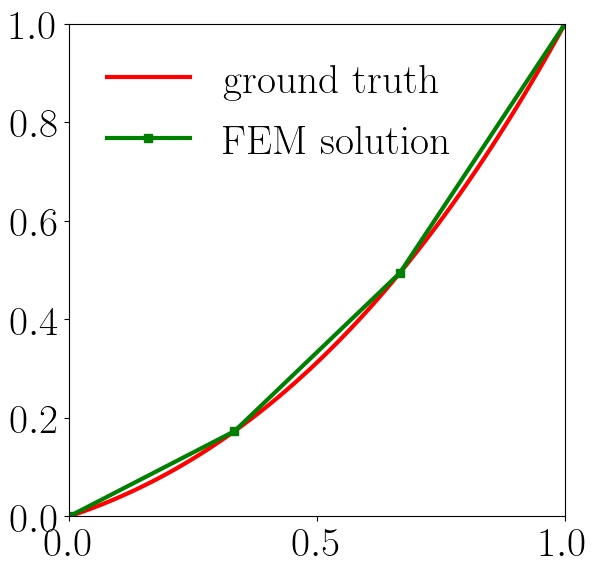
\includegraphics[width=.3\linewidth]{fem.png}
	\caption{The ground truth $\varphi(x) = \frac{1}{6} x^3 + \frac{1}{2} x^2 + \frac{1}{3} x$ and its approximation found by the FEM.}
	\label{fig:fem}
%\end{minipage}
%\hspace{.1\linewidth}
%\begin{minipage}{.45\linewidth}
%	\centering
%	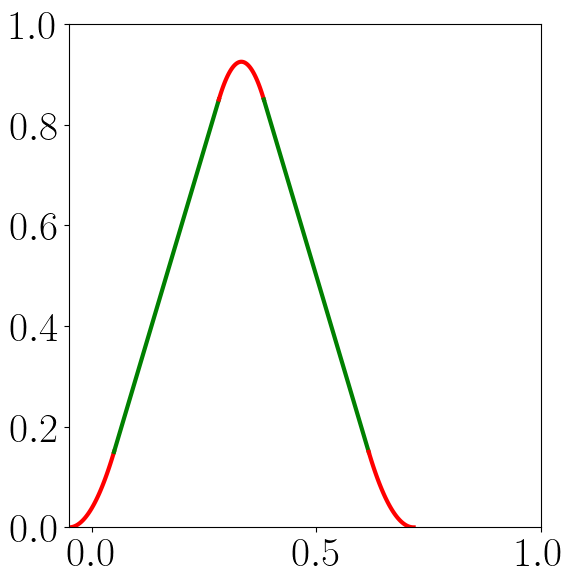
\includegraphics[width=.8\linewidth]{convolution.png}
%	\caption{}
%	\label{fig:convolution}
%\end{minipage}
\end{figure}

\subsection{The Ritz method}
Let us see another method to solve the problem~\eqref{eq:femproblem}. 
The Ritz method seeks to minimize the total potential energy $\Phi(\tilde\varphi) := ( \tilde\varphi, \mathcal A \tilde\varphi) - 2 (\tilde\varphi, f)$.
For our particular problem it can be written as follows:
\begin{equation}
\label{eq:ritz}
\argmin\limits_{b,c\in \mathbb R} \Phi(\tilde\varphi), \text{~where~} \Phi(\tilde\varphi) :=  \int\limits_0^1 \tilde\varphi \frac{d^2}{dx^2}\tilde{\varphi}\, dx -2 \int\limits_0^1 \tilde\varphi f\ \, dx 
\end{equation}

To find the minimum, we set the partial derivatives to zero:
\begin{equation}
\label{eq:ritz}
\left\{
\begin{split}
\frac{\partial}{\partial b} \Phi(\tilde\varphi) & = 0 \\
\frac{\partial}{\partial c} \Phi(\tilde\varphi) & = 0
\end{split}
\right.
\end{equation}

%$$
%\tilde{\varphi}(x) := 0\cdot w_0(x) + b\cdot w_1(x) + c\cdot w_2(x) + 1\cdot w_3(x),
%$$
Let us denote the Dirac delta centered at point $y$ as $\delta_y(x)$; then $\frac{d^2\tilde{\varphi}}{dx^2}$ has the following expression:
$$
\frac{d^2\tilde{\varphi}}{dx^2} = 3b(\delta_0(x) - 2\delta_{1/3}(x) + \delta_{2/3}(x)) + 3c(\delta_{1/3}(x) - 2\delta_{2/3}(x) + \delta_{1}(x)) + 3\delta_{2/3}(x)
$$

It is straightforward to compute the potential energy:
\begin{align*}
\Phi(\tilde\varphi) &= \int\limits_0^1 \tilde{\varphi} \cdot \left(\frac{d^2\tilde{\varphi}}{dx^2} - 2(x+1)\right)\,dx \\
&= \int\limits_0^1 (b w_1 + c w_2 + w_3 ) \cdot (3b(\delta_0 - 2\delta_{1/3} + \delta_{2/3}) + 3c(\delta_{1/3} - 2\delta_{2/3} + \delta_{1}) + 3\delta_{2/3} - 2(x+1))\,dx \\
&= -6b^2 + 6bc -6c^2 + 6c -2\left(\frac{5}{9}c + \frac{4}{9}b + \frac{49}{54}\right)
\end{align*}

By equating the partial derivatives to zero, the system~\ref{eq:ritz} can be reduced to:
$$
\left\{
\begin{split}
2b - c &= -\frac{4}{27}\\
-b + 2c &= \frac{22}{27}
\end{split}
\right.
$$

Note that this is exaclty the same system as~\eqref{eq:galerkin:bc}!
It turns out that for equations with self-adjoint positive definite operator ($-\frac{d^2}{dx^2}$ satisfies the conditions),
the Galerkin formulation results in the same system of equations as in the Ritz formulation.
A proof of this fact is out of scope of the present document; we can, however, demonstrate it for our problem~\eqref{eq:femproblem} approximated with the hat functions.

\iffalse
(%i1) integrate(3*x*(x+1),x,0,1/3);
                                      11
(%o1)                                 --
                                      54
(%i2) integrate(3*x*(x+1),x,0,1/3) + integrate((2-3*x)*(x+1),x,1/3,2/3);
                                       4
(%o2)                                  -
                                       9
(%i3) integrate((3*x-1)*(x+1),x,1/3,2/3);
                                      7
(%o3)                                 --
                                      27
(%i4) integrate((3*x-1)*(x+1),x,1/3,2/3) + integrate((3-3*x)*(x+1),x,2/3,1) ;
                                       5
(%o4)                                  -
                                       9
(%i5) integrate((4-3*x)*(x+1),x,2/3,1);
                                      49
(%o5)                                 --
                                      54
(%i6) b*(integrate(3*x*(x+1),x,0,1/3) + integrate((2-3*x)*(x+1),x,1/3,2/3))+ c*(integrate((3*x-1)*(x+1),x,1/3,2/3) + integrate((3-3*x)*(x+1),x,2/3,1))+ integrate((4-3*x)*(x+1),x,2/3,1);
                                5 c   4 b   49
(%o6)                           --- + --- + --
                                 9     9    54
(%i7) f:-6*b^2;
                                         2
(%o7)                               - 6 b
(%i8) f:-6*b^2 + 6*b*c -6*c^2 +6*c -2*(5/9*c + 4/9*b + 49/54);
                    2                     5 c   4 b   49       2
(%o8)         (- 6 c ) + 6 b c + 6 c - 2 (--- + --- + --) - 6 b
                                           9     9    54
(%i9) diff(f, c);
                                               44
(%o9)                         (- 12 c) + 6 b + --
                                               9
(%i10) diff(f, b);
                                             8
(%o10)                          6 c - 12 b - -
                                             9
(%i11) 44/54;
                                      22
(%o11)                                --
                                      27
(%i12) 8/54;
                                      4
(%o12)                                --
                                      27
(%i13)

% \frac{\partial}{\partial c} \Phi(\tilde\varphi) & = 0
%radcan(
%   integrate((3*x+3*e-2+1)^2/(12*e)*(-b*3/e+c*3/(2*e)), x, 1/3-e, 1/3+e) +
%   integrate((1-(3*x-2)^2-(3*e-1)^2)/(6*e)*(b*3/(2*e)-c*3/e+3/(2*e)), x, 2/3-e, 2/3+e) +
%   integrate((3*x-3*e-2-1)^2/(12*e)*(c*3/(2*e)-3/e), x, 1-e, 1+e) +

%-2*integrate((3*x+3*e-2+1)^2/(12*e)*(x+1),              x, 1/3-e, 1/3+e) +
%-2*integrate((3*x-2+1)*(x+1), x, 1/3+e, 2/3-e) +
%-2*integrate((1-(3*x-2)^2-(3*e-1)^2)/(6*e)*(x+1),                     x, 2/3-e, 2/3+e) +
%-2*integrate((-3*x+2+1)*(x+1), x, 2/3+e, 1-e) +
%-2*integrate((3*x-3*e-2-1)^2/(12*e)*(x+1),           x, 1-e, 1+e) +

%   integrate((b*((1-(3*x-1)^2-(3*e-1)^2)/(6*e)) + c*(3*x+3*e-2+1)^2/(12*e))*(3/(2*e)), x, 1/3-e, 1/3+e) +
%   integrate((b*(((3*x-3*e-1-1)^2)/(12*e)) + c*(1-(3*x-2)^2-(3*e-1)^2)/(6*e) + (3*x+3*e - 3 +1)^2/(12*e))*(-3/e), x, 2/3-e, 2/3+e) +
%   integrate((c*(3*x-3*e-2-1)^2/(12*e) + (1-(3*x-3)^2 - (3*e-1)^2)/(6*e))*(3/(2*e)), x, 1-e, 1+e)
%);

b*(integrate(3*x*(x+1),x,0,1/3) + integrate((2-3*x)*(x+1),x,1/3,2/3))+ c*(integrate((3*x-1)*(x+1),x,1/3,2/3) + integrate((3-3*x)*(x+1),x,2/3,1))+ integrate((4-3*x)*(x+1),x,2/3,1);
\fi

\section{DIY PDE solution}
All these FEM approaches are very fancy, let us cobble together a simpler solution.
Let us represent the solution by $n+1$ samples; we sample the function uniformly over the domain at the points $\{x_i\}_{i=0}^n = \left\{\frac{i}{n}\right\}_{i=0}^n$.
So, we want to compute $n+1$ samples $\begin{pmatrix}\tilde\varphi(0) & \tilde\varphi\left(\frac{1}{n}\right) & \tilde\varphi\left(\frac{2}{n}\right) & \dots &\tilde\varphi(1) \end{pmatrix}^\top$, where the first and the last one are fixed.
Note that for the case of the hat functions basis, computing $\tilde\varphi(x_i)$ corresponds exactly to the computation of the weights in Equation~\eqref{eq:tildephi}.

We can approximate the differential operator $\mathcal A$ by the second-order central finite difference:
$$\frac{d^2}{dx^2}\tilde\varphi\left(\frac{i}{n}\right) \approx \frac{\tilde\varphi\left(\frac{i-1}{n}\right) -2\tilde\varphi\left(\frac{i}{n}\right)+\tilde\varphi\left(\frac{i+1}{n}\right)  }{\frac{1}{n^2}}.$$


Since $\tilde\varphi(0)$ and $\tilde\varphi(1)$ are fixed, all this boils down to the following system of $n-1$ equations:
$$
\begin{pmatrix}
-2 n^2 &   n^2 &       &      &      &       &        \\
   n^2 & -2n^2 & n^2   &      &      &       &        \\
       &       &       &\ddots&      &       &        \\
       &       &       &      &  n^2 & -2n^2 &    n^2 \\
       &       &       &      &      &   n^2 & -2 n^2
\end{pmatrix}
\begin{pmatrix}[1.5] \tilde\varphi\left(\frac{1}{n}\right) \\ \tilde\varphi\left(\frac{2}{n}\right) \\ \vdots \\\tilde\varphi\left(\frac{n-1}{n}\right) \end{pmatrix}
=
\begin{pmatrix}[1.5] f\left(\frac{1}{n}\right) - n^2 \tilde\varphi(0) \\ f\left(\frac{2}{n}\right) \\ \vdots \\\ f\left(\frac{n-1}{n}\right) - n^2\tilde\varphi(1) \end{pmatrix}
$$

Let us precompute the right-hand side $f\left(\frac{i}{n}\right) = \frac{i}{n} + 1$, and with minor simplifications our system can be transformed as follows:
$$
\underbrace{\begin{pmatrix}
 2     & -1    &       &      &      &       &        \\
-1     &  2    &  -1   &      &      &       &        \\
       &       &       &\ddots&      &       &        \\
       &       &       &      &  -1  &  2    & -1     \\
       &       &       &      &      &  -1   &  2
\end{pmatrix}}_{:= A}
\underbrace{\begin{pmatrix}[1.5] \tilde\varphi\left(\frac{1}{n}\right) \\ \tilde\varphi\left(\frac{2}{n}\right) \\ \vdots \\\tilde\varphi\left(\frac{n-1}{n}\right) \end{pmatrix}}_{:=x}
=
\underbrace{\begin{pmatrix}[1.5] -\frac{1+n}{n^3} + \tilde\varphi(0) \\ \-\frac{2+n}{n^3} \\ \vdots \\\ -\frac{n-1+n}{n^2} +\tilde\varphi(1) \end{pmatrix}}_{:=b}
$$

This is a simple linear system $Ax=b$\footnote{Note that we have redefined $b$, it is not a scalar anymore but the right-hand side vector.} with a symmetric positive definite matrix $A$.
It is not very surprising to see that this system is again exactly the same as~\eqref{eq:galerkin:bc}.
The Galerkin method corresponds to solving this system directly, whereas the Ritz method corresponds to minimization of the quadratic form $x^\top A x - 2b^\top x$.
It turns out that in the case of a symmetric positive definite matrix $A$ both solving for $Ax=b$ and minimizing the quadratic form $x^\top A x - 2b^\top x$ are equivalent;
the following chapter is dedicated to this remarkable fact.

\authoredby{B}
\chapter{Minimization of quadratic functions and linear systems}
\fancyhead[R]{\textcolor{ao(english)}{core text}}
\label{sec:mineqlin}

Recall that the main goal is to study least squares, therefore our main tool will be the minimization of quadratic functions;
however, before we start using this power tool, we need to find where its on/off button is located.
First of all, we need to recall what a matrix is; then we will revisit the definition of a positive numbers, and only then we will attack minimization of quadratic functions.

\section{Matrices and numbers}
In this sections, matrices will be omnipresent, so let's remember what it is.
Do not peek further down the text, pause for a few seconds, and try to formulate what the matrix is.

\subsection{Different interpretations of matrices}

The answer is very simple. A matrix is just a locker that stores stuff.
Each piece of stuff lies in its own cell, cells are grouped in rows and columns.
In our particular case, we store real numbers; for a programmer the easiest way to imagine a matrix $A$ is something like:
\begin{minted}{cpp}
float A[m][n];
\end{minted}

Why would we need a storage like this? What does it describe?
Maybe I will upset you, but the matrix by itself does not describe anything, it stores stuff.
For example, you can store coefficients of a function in it.
Let us put aside matrices for a second imagine that we have a number $a$. What does it mean?
Who knows what it means\dots For example, it can be a coefficient inside a function that takes one number as an input and gives another number as an output:
$$
f(x) : \mathbb R \rightarrow \mathbb R
$$

One possible instance of such a function a mathematicion could write down as:
$$
f(x) = ax
$$

In the programmers' world it would look something like this:
\begin{minted}[linenos=true]{cpp}
float f(float x) {
    return a*x;
}
\end{minted}

On the other hand, why this function and not another one? Let's take another one!
$$
f(x) = ax^2
$$
A programmer would write it like this:
\begin{minted}[linenos=true]{cpp}
float f(float x) {
    return x*a*x;
}
\end{minted}

One of these functions is linear and the other is quadratic. Which one is correct? 
Neither one. The number $a$ does not define it, it just stores a value! 
Build the function you need.

The same thing happens to matrices, they give storage space when simple numbers (scalars) do not suffice, a matrix is a sort of an hyper-number.
The addition and multiplication operations are defined over matrices just as over numbers.
%. The division is a bit more complicated, but in certain cases it can be defined too.

Let us suppose that we have a $2\times 2$ matrix $A$:
$$
A=\begin{bmatrix} a_{11} & a_{12} \\ a_{21} & a_{22}\end{bmatrix}
$$

The matrix does not mean anything by itself, for example, it can be interpreted as a linear function:
$$
f(x) : \mathbb R^2 \rightarrow \mathbb R^2, \quad f(x) = Ax
$$

Here goes the programmer's view on the function:
\begin{minted}[linenos=true]{cpp}
vector<float> f(vector<float> x) {
    return vector<float>{a11*x[0] + a12*x[1],  a21*x[0] + a22*x[1]};
}
\end{minted}

This function maps a two-dimensional vector to a two-dimensional vector.
Graphically, it is convenient to imagine it as an image transformation: we give an input image, and the output is the stretched and/or rotated (maybe even mirrored!) version.
The top row of Figure~\ref{fig:matrices} provides few different examples of this interpretation of matrices.

On the other hand, nothing prevents to interpret the matrix $A$ as a function that maps a vector to a scalar:
$$
f(x) : \mathbb R^2 \rightarrow \mathbb R, \quad f(x) = x^\top A x = \sum\limits_i\sum\limits_j a_{ij}x_i x_j
$$

Note that the square is not very well defined for the vectors, so I cannot write $x^2$ as I wrote in the case of ordinary numbers. 
For those who are not at ease with matrix multiplications, I highly recommend to revisit it right now and check that the expression $x^\top A x$ indeed produces a scalar value.
To this end, we can explicitly put brackets $x^\top A x = (x^\top A) x$.
Recall that in this particular example $x$ is a two-dimensional vector (stored in a $2\times 1$ matrix).
Let us write all the matrix dimensions explicitly:
$$
\underbrace{\underbrace{\left(\underbrace{x^\top}_{1\times 2} \times \underbrace{A}_{2\times 2}\right)}_{1\times 2} \times \underbrace{x}_{2\times 1}}_{1 \times 1}
$$

Returning to the cozy world of programmers, we can write the same quadratic function as follows:
\begin{minted}[linenos=true]{cpp}
float f(vector<float> x) {
    return x[0]*a11*x[0] + x[0]*a12*x[1] + x[1]*a21*x[0] + x[1]*a22*x[1];
}
\end{minted}

\begin{figure}[ht]
	\centering
	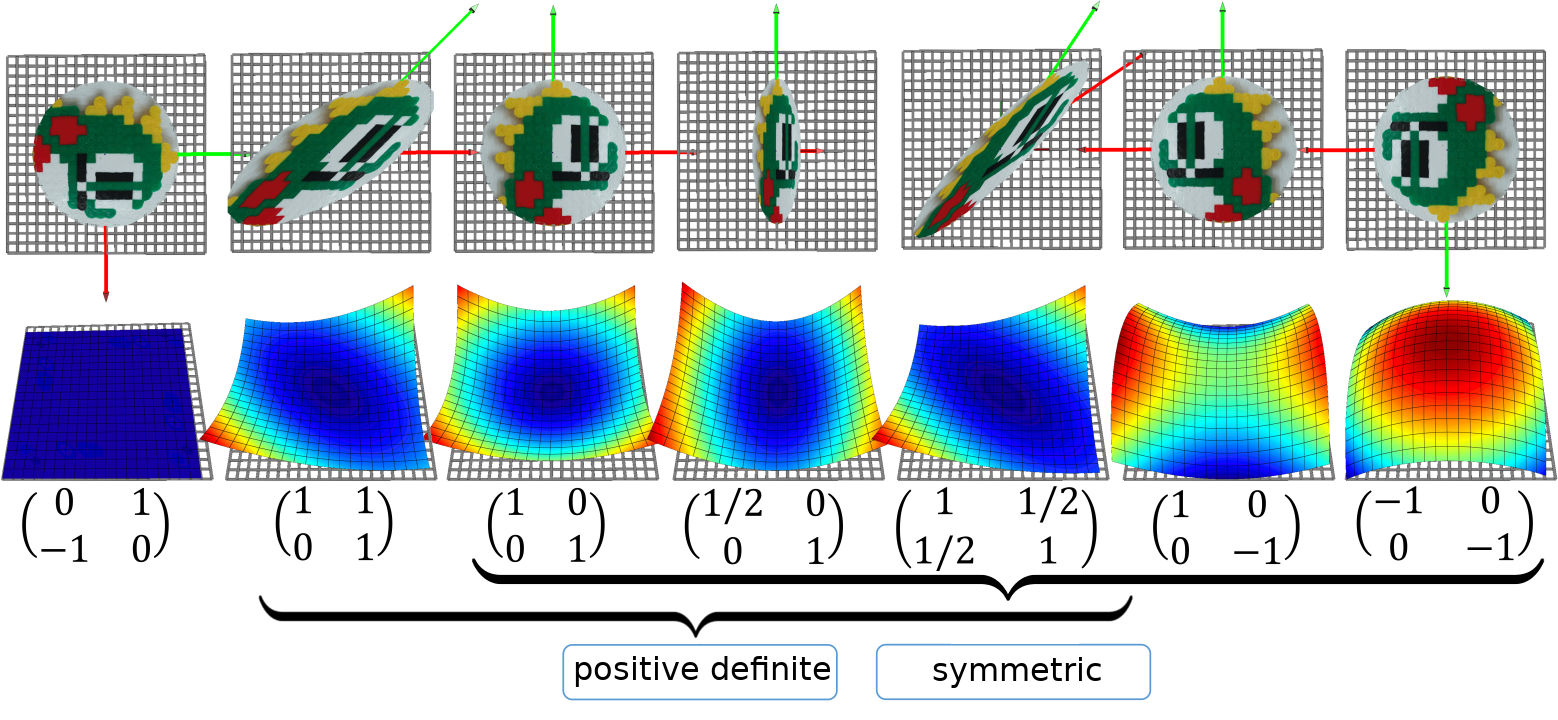
\includegraphics[width=\linewidth]{matrices}
	\caption{Seven examples of $2\times 2$ matrices, some of them are positive definite and/or symmetric. 
    \textbf{Top row:} the matrices are interpreted as linear functions $f(x):\mathbb R^2 \rightarrow \mathbb R^2$. \textbf{Middle row:} the matrices are interpreted as quadratic functions
 $f(x):\mathbb R^2 \rightarrow \mathbb R$.}
	\label{fig:matrices}
\end{figure}


\subsection{What is a positive number?}
Allow me to ask a very stupid question: what is a positive number?
We have a great tool called the predicate ``greater than'' $>$.
Do not be in a hurry to answer that the number $a$ is positive if and only if $a>0$, it would be too easy. Let us define the positivity as follows:

\begin{definition}
The real number $a$ is positive if and only if for all non-zero real $x\in\mathbb R,\ x\neq 0$ the condition $ax^2>0$ is satisfied.
\end{definition}

This definition looks pretty awkward, but it applies perfectly to matrices:

\begin{definition}
The square matrix $A$ is called positive definite if for any non-zero $x$
the condition $x^\top A x > 0$ is met, i.e. the corresponding quadratic form is strictly positive everywhere except at the origin.
\end{definition}

What do we need the positivity for?
As we have already mentioned, our main tool will be the minimization of quadratic functions. 
It would be nice to be sure that the minimum exists!
For example, the function $f(x) = - x^2$ clearly has no minimum, because the number -1 is not positive, 
both branches of the parabola $f(x)$ look down.
Positive definite matrices guarantee that the corresponding quadratic forms form a paraboloid with a (unique) minimum.
Refer to the Figure~\ref{fig:matrices} for an illustration.

Thus, we will work with a generalization of positive numbers, namely, positive definite matrices. 
Moreover, in our particular case, the matrices will be symmetric!
Note that quite often, when people talk about positive definiteness, they also imply symmetry.
This can be partly explained by the following observation (optional for the understanding of the rest of the text):

\subsubsection{A digression on quadratic forms and matrix symmetry}

Let us consider a quadratic form $x^\top M x$ for an arbitrary matrix $M$. 
Next we add and subtract a half ot its transpose:
$$
M = \underbrace{\frac{1}{2} (M+M^\top)}_{:=M_s} + \underbrace{\frac{1}{2} (M-M^\top)}_{:=M_a} = M_s + M_a
$$

The matrix $M_s$ is symmetric: $M_s^\top = M_s$; the matrix $M_a$ is antisymmetric: $M_a^\top=-M_a$.
A remarkable fact is that for any antisymmetric matrix the corresponding quadratic form is equal to zero everywhere. This follows from the following observation:
$$
q = x^\top M_a x  = (x^\top M_a^\top x)^\top = - (x^\top M_a x)^\top = -q
$$
It means that the quadratic form $x^\top M_a x$ equals $q$ and $-q$ at the same time, and the only way to have this condition is to have $q\equiv 0$.
From this fact it follows that for an arbitrary matrix $M$ the corresponding quadratic form $x^\top M x$ can be expressed through the symmetric matrix $M_s$ as well:
$$
x^\top M x = x^\top (M_s + M_a) x = x^\top M_s x  + x^\top M_a x = x^\top M_s x.
$$


\section{Minimizing a quadratic function}

\begin{figure}[ht]
	\centering
	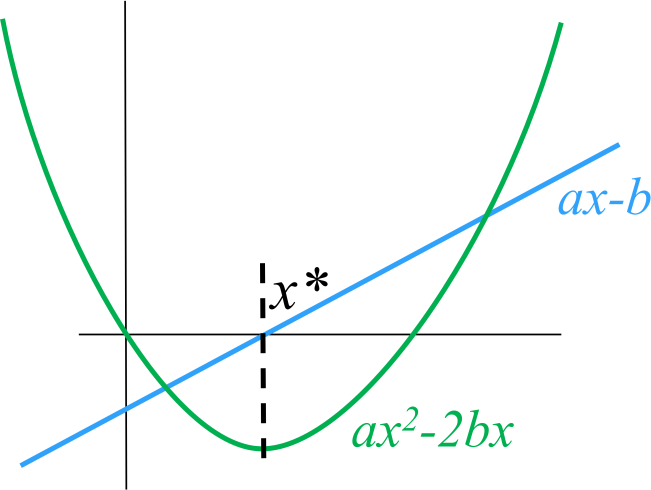
\includegraphics[width=.3\linewidth]{minpb1d}
	\caption{In 1d, the solution $x^*$ of the equation $ax - b = 0$ solves the minimization problem $\argmin\limits_x(ax^2-2bx)$ as well. }
	\label{fig:min1d}
\end{figure}

Let us return to the unidimensional world for a while; I want to find the minimum of the function $f(x) = ax^2 - 2bx$. 
The number $a$ is positive, therefore the minimum exists; to find it, we equate with the corresponding derivative with zero: $\frac{d}{dx}f(x) = 0$. 
It is easy to differentiate a unidimensional quadratic function: $\frac{d}{dx}f(x) = 2ax - 2b = 0$; so our problem boils down to the equation $ax-b=0$.
With some effort we can find the solution $x^* = b/a$. Figure~\ref{fig:min1d} illustrates the equivalence of two problems:
the solution $x^*$ of the equation $ax-b=0$ coincides with the minimizer $\argmin\limits_x(ax^2 - 2bx)$.

My point is that our main goal is to minimize quadratic functions (we are talking about least squares here!).
The only thing that the humanity knows to do well is to solve linear equations, and it is great that one is equivalent to the other!
The last thing is to check whether this equivalence holds for the case of $n>1$ variables.
To do so, we will first prove three theorems.

\subsection{Three theorems, or how to differentiate matrix expressions}
The first theorem states that $1\times 1$ matrices are invariant w.r.t the transposition:
\begin{theorem}
$x\in \mathbb R \Rightarrow x^\top = x$
\end{theorem}
The proof is left as an exercise.

The second theorem allows us to differentiate linear functions. In the case of a real function of one variable we know that
$\frac{d}{dx}(bx) = b$, but what happens in the case of a real function of $n$ variables?
\begin{theorem}
$\nabla b^\top x = \nabla x^\top b = b$
\end{theorem}
No surprises here, the same result in a matrix notation. The proof is straightforward, it suffices to write down the definition of the gradient:
$$\nabla(b^\top x) = \begin{bmatrix}\frac{\partial (b^\top x)}{\partial x_1} \\ \vdots \\ \frac{\partial (b^\top x)}{\partial x_n} \end{bmatrix} = \begin{bmatrix}\frac{\partial (b_1 x_1 + \dots + b_n x_n)}{\partial x_1} \\ \vdots \\ \frac{\partial (b_1 x_1 + \dots + b_n x_n)}{\partial x_n} \end{bmatrix}
= \begin{bmatrix}b_1 \\ \vdots \\ b_n \end{bmatrix} = b$$
Now applying the first theorem: $b^\top x = x^\top b$, and this concludes the proof.

Now let us switch to quadratic forms.
We know that in the case of a real function of one variable we have $\frac{d}{dx}(ax^2) = 2ax$, but what happens with the quadratic forms?
\begin{theorem}
$\nabla (x^\top A x) = (A+A^\top)x$
\end{theorem}
Note that if $A$ is symmetric, then $\nabla (x^\top A x) = 2Ax$.
The proof is straightforward, let us express the quadratic form as a double sum:
$$x^\top A x = \sum\limits_i\sum\limits_j a_{ij} x_i x_j$$
Now let us differentiate this double sum w.r.t the variable $x_i$:
\begin{align*}
\frac{\partial (x^\top A x)}{\partial x_i} 
&= \frac{\partial}{\partial x_i}  \left(\sum\limits_{k_1}\sum\limits_{k_2} a_{k_1 k_2} x_{k_1} x_{k_2}\right) = \\
&= \frac{\partial}{\partial x_i}  \left(
\underbrace{\sum\limits_{k_1\neq i}\sum\limits_{k_2\neq i} a_{ik_2}x_{k_1} x_{k_2}}_{k_1 \neq i, k_2 \neq i}+\underbrace{\sum\limits_{k_2\neq i} a_{ik_2}x_i x_{k_2}}_{k_1 = i, k_2\neq i}+
\underbrace{\sum\limits_{k_1\neq i} a_{k_1 i} x_{k_1} x_i}_{k_1 \neq i, k_2 = i}+
\underbrace{a_{ii}x_i^2}_{k_1 = i, k_2 = i}\right) = \\
& = \sum\limits_{k_2\neq i} a_{ik_2}x_{k_2} + \sum\limits_{k_1\neq i} a_{k_1 i} x_{k_1} + 2 a_{ii} x_i = \\
& = \sum\limits_{k_2} a_{ik_2}x_{k_2} + \sum\limits_{k_1} a_{k_1 i} x_{k_1} = \\
& = \sum\limits_{j} (a_{ij} + a_{ji}) x_j \\
\end{align*}
I split the double sum into four cases, shown by the curly brackets.
Each of these four cases is trivial to differentiate. 
Now let us collect the partial derivatives  into a gradient vector:
$$\nabla(x^\top A x) = \begin{bmatrix}\frac{\partial (x^\top Ax)}{\partial x_1} \\ \vdots \\ \frac{\partial (x^\top A x)}{\partial x_n} \end{bmatrix}  = \begin{bmatrix}\sum\limits_{j} (a_{1j} + a_{j1}) x_j \\ \vdots \\ \sum\limits_{j} (a_{nj} + a_{jn}) x_j \end{bmatrix}  = (A+A^\top)x
$$

\subsection{Minimum of a quadratic function and the linear system}
Recall that for a positive real number $a$ solving the equation
$ax=b$ is equivalent to the quadratic function $\argmin\limits_x(ax^2 - 2bx)$ minimization.

We want to show the corresponding connection in the case of a symmetric positive definite matrix $A$.
So, we want to find the minimum quadratic function
$$\argmin\limits_{x\in\mathbb R^n} (x^\top A x - 2b^\top x).$$
As before, let us equate the derivative to zero:
$$\nabla (x^\top A x - 2b^\top x) = \begin{bmatrix}0 \\ \vdots \\ 0 \end{bmatrix}.$$
The Hamilton operator is linear, so we can rewrite our equation as follows:
$$\nabla (x^\top A x) - 2\nabla(b^\top x) = \begin{bmatrix}0 \\ \vdots \\ 0 \end{bmatrix}.$$
Now let us apply the second and third differentiation theorems:
$$(A+A^\top)x - 2b = \begin{bmatrix}0 \\ \vdots \\ 0 \end{bmatrix}.$$
Recall that $A$ is symmetric, let us divide the equation by 2, and we obtain the final linear system:
$$Ax = b.$$
Hurray, passing from one variable to many, we have not lost a thing, and can effectively minimize quadratic functions!

%$$\argmin (x^\top A x - 2b^\top x) = A^{-1}b$$

\section{Back to the least squares}
Finally we can move on to the main content of this course. Imagine that we have two points on a plane
$(x_1, y_1)$ and $(x_2, y_2)$, and we want to find an equation for the line passing through these two points.
The equation of the line can be written as $y = \alpha x + \beta$, that is, our task is to find the coefficients $\alpha$ and $\beta$.
This is a secondary school exercise, let us write down the system of equations:
$$
\left\{
\begin{split}
\alpha x_1 + \beta &= y_1\\
\alpha x_2 + \beta &= y_2\\
\end{split}
\right.
$$

We have two equations with two unknowns ($\alpha$ and $\beta$), the rest is known.
In general, there exists a unique solution. For convenience, let's rewrite the same system in a matrix form:
$$
\underbrace{\begin{bmatrix}x_1  & 1 \\ x_2 & 1 \end{bmatrix}}_{:=A} 
\underbrace{\begin{bmatrix} \alpha \\ \beta \end{bmatrix}}_{:=x} = \underbrace{\begin{bmatrix} y_1 \\ y_2 \end{bmatrix}}_{:=b}
$$
We obtain the equation $Ax = b$, which is trivially soved as $x^* = A^{-1}b$.

And now let us imagine that we have \textbf{three} points through which we need to draw a straight line:
$$
\left\{
\begin{split}
\alpha x_1 + \beta &= y_1\\
\alpha x_2 + \beta &= y_2\\
\alpha x_3 + \beta &= y_3\\
\end{split}
\right.
$$

In a matrix form, this system can be expressed as follows:
$$
\underbrace{\begin{bmatrix}x_1  & 1 \\ x_2 & 1 \\x_3 & 1 \end{bmatrix} }_{:= A\,(3\times 2)}
\underbrace{\begin{bmatrix} \alpha \\ \beta \end{bmatrix}}_{:=x\,(2\times 1)} = \underbrace{\begin{bmatrix} y_1 \\ y_2 \\ y_3 \end{bmatrix}}_{:=b\, (3\times 1)}
$$

The matrix $A$ is rectangular, and thus it is not invertible!
Sounds legit, we have only two variables and three equations, and in general this system has no solution.
This is a perfectly normal situation in the real world where the data comes from noisy measurements,
and we need to find the parameters $\alpha$ and $\beta$ that fit the measurements the best.
We have already encountered this situation in \S\ref{sec:springscale}, where we calibrated a spring scale.
However, back then the solution we have obtained was purely algebraic and very cumbersome. Let's try a more intuitive way.

Our system can be written down as follows:
$$
\alpha \underbrace{\begin{bmatrix}x_1  \\ x_2 \\x_3  \end{bmatrix} }_{:=\vec{i}}
+\beta \underbrace{\begin{bmatrix}1 \\ 1 \\1 \end{bmatrix} }_{:=\vec{j}} = 
\begin{bmatrix}y_1\\y_2\\y_3\end{bmatrix}
$$
Or, in more shortly,
$$
\alpha \vec{i} + \beta\vec{j} = \vec{b}.
$$
The vectors $\vec i$, $\vec j$ and $\vec b$ are known, we are looking for (unknown) scalars $\alpha$ and $\beta$.
Obviously, the linear combination $\alpha \vec{i} + \beta\vec{j}$ generates a plane, and if the vector $\vec b$
does not lie in this plane, there is no exact solution; however, we are looking for an \textit{approximate} solution.

Let's denote the solution error as $\vec{e}(\alpha, \beta) :=  \alpha \vec{i} + \beta\vec{j} - \vec b$.
Our goal is to find the values of parameters $\alpha$ and $\beta$ that minimize the norm of the vector $\vec{e}(\alpha, \beta)$. 
In other words, the problem can be formulated as $\argmin\limits_{\alpha, \beta} \|\vec{e}(\alpha, \beta)\|$.
Refer to Fig.~\ref{fig:error} for an illustration.

\begin{figure}[ht]
	\centering
	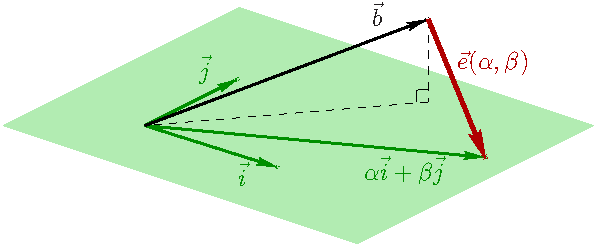
\includegraphics[width=.7\linewidth]{error.pdf}
	\caption{Given the vectors $\vec i$, $\vec j$ and $\vec b$, we want to minimize the norm of the error vector $\vec e$. 
    Obviously the norm is minimized when the vector is orthogonal to the plane generated by $\vec i$ and $\vec j$.}
	\label{fig:error}
\end{figure}

But wait, where are the least squares? Just a second. The square root function $\sqrt{\cdot}$ is monotonous, so $\argmin\limits_{\alpha, \beta} \|\vec{e}(\alpha, \beta)\|$ = $\argmin\limits_{\alpha, \beta} \|\vec{e}(\alpha, \beta)\|^2$!

It is quite obvious that the norm of the error vector is minimized when it is orthogonal to the plane generated by the vectors $\vec i$ and $\vec j$.
We can express it by equating corresponding dot products to zero:
$$
\left\{
\begin{split}\vec{i}^\top \vec{e}(\alpha, \beta) &= 0\\
\vec{j}^\top \vec{e}(\alpha, \beta) &= 0
\end{split}
\right.
$$

We can write down the same system in a matrix form:
$$
\begin{bmatrix}x_1 & x_2 & x_3 \\ 1 & 1 & 1 \end{bmatrix}
\left(\alpha \begin{bmatrix}x_1  \\ x_2 \\x_3  \end{bmatrix}
+\beta \begin{bmatrix}1 \\ 1 \\1 \end{bmatrix} - 
\begin{bmatrix}y_1\\y_2\\y_3\end{bmatrix}\right) = \begin{bmatrix}0\\0\end{bmatrix}
$$
or
$$
\begin{bmatrix}x_1 & x_2 & x_3 \\ 1 & 1 & 1 \end{bmatrix}
\left(
\begin{bmatrix}x_1  & 1 \\ x_2 & 1 \\x_3 & 1 \end{bmatrix}
\begin{bmatrix} \alpha \\ \beta \end{bmatrix}-
\begin{bmatrix} y_1 \\ y_2 \\ y_3 \end{bmatrix}
\right) = \begin{bmatrix}0\\0\end{bmatrix}
$$
But we won't stop there, because the expression can be further shortened:
$$
A^\top (Ax - b)= \begin{bmatrix}0\\0\end{bmatrix}
$$
And the very last transformation:
$$
A^\top Ax = A^\top b.
$$
Let us do a sanity check. Matrix $A$ is $3\times 2$, thus  $A^\top A$ is $2\times 2$. Matrix $b$ is $3\times 1$, so the matrix $A^\top b$ is $2\times 1$.
Therefore, in a general case the matrix $A^\top A$ can be invertible! Moreover, $A^\top A$ has a couple more nice properties.

\begin{theorem}
$A^\top A$ is symmetric.
\end{theorem}
It is very easy to show:
$$
(A^\top A)^\top = A^\top (A^\top)^\top = A^\top A.
$$

\begin{theorem}
	$A^\top A$ positive semidefinite: $\forall x\in \mathbb R^n\quad x^\top A^\top A x \geq 0.$
\end{theorem}
It follows from the fact that $x^\top A^\top A x = (A x)^\top A x > 0$.
Moreover, $A^\top A$ is positive definite in the case where $A$ has linearly independent columns (rank $A$ is equal to the number of the variables in the system).

\vspace{5mm}

Congratulations, we have just found another way to do the spring scale calibration (\S\ref{sec:springscale}).
For a system with two unknowns, we have proven that to minimize the quadratic function $\argmin\limits_{\alpha, \beta} \|\vec{e}(\alpha, \beta)\|^2$
is equivalent to solve the linear system $A^\top A x = A^\top b$.
Of course, all this reasoning applies to any other number of variables, but let us write it all down again a compact algebraic way.
Let us start with a least squares problem:
\begin{align*}
\argmin \| Ax - b \|^2 &= \argmin (Ax-b)^\top (Ax-b) =\\
& = \argmin\left(x^\top A^\top - b^\top\right)(Ax-b) = \\
& = \argmin\left(x^\top A^\top A x - b^\top Ax - x^\top A^\top b + \underbrace{b^\top b}_{\rm const}\right)=\\
& = \argmin\left(x^\top A^\top A x - 2b^\top Ax\right) = \\
& = \argmin\left(x^\top \underbrace{\left(A^\top A\right)}_{:=A'} x - 2\underbrace{\left(A^\top b\right)}_{:=b'}\phantom{}^\top x\right)
\end{align*}
Having started with a least squares problem, we have come to the quadratic function minimization problem we know already.
Thus, the least squares problem $\argmin \| Ax - b \|^2$  is equivalent to minimizing the quadratic function $\argmin \left(x^\top A' x - 2b'^\top x\right)$ 
with (in general) a symmetric positive definite matrix $A'$, which in turn is equivalent to solving a system of linear equations $A'x = b'$. Phew. The theory is over.


%\chapter{Finite elements example: the Ritz method}


\chapter{Least squares through examples}

\section{Linear-quadratic regulator}
\label{sec:lqr}
Let us start this chapter with a tiny example from the optimal control theory.
Optimal control deals with the problem of finding a control law for a given system such that a certain optimality criterion is achieved.
This phrase is too unspecific, let us illustrate it.
Imagine that we have a car that advances with some speed, say $0.5$m/s. The goal is to accelerate and reach, say, $2.3$m/s.
We can not control the speed directly, but we can act on the acceleration via the gas pedal.
We can model the system with a very simple equation:
$$
v_{k+1} = v_k + u_k,
$$
where the signals are sampled every 1 second, $v_k$ is the car speed and $u_k$ is the acceleration of the car.
Let us say that we have half a minute to reach the given speed, i.e, $v_0=0.5$m/s, $v_n=2.3$m/s, $n=30$s.
So, we need to find $\{u_i\}_{i=0}^{n-1}$ that optimizses some quality criterion $J(\vec{v}, \vec{u})$:
$$
\min J(\vec{v},\vec{u}) \quad s.t.~  v_{i+1} = v_i + u_i ~~ \forall i \in 0..n-1
$$
The case where the system dynamics are described by a set of differential equations and the cost is described by a quadratic functional is called a linear quadratic problem.
Let us test few different quality criteria. What happens if we ask for the car to reach the final speed as quickly as possible?
It can be written as follows:
$$
J(\vec{v}, \vec{u}) := \sum\limits_{i=1}^n (v_i-v_n)^2 = \sum\limits_{i=1}^n \left(\sum\limits_{j=0}^{i-1}u_j-v_n+v_0\right)^2
$$

To minimize this criterion, we can solve the following system in the least squares sense:
$$
\left \{ \begin{array}{ccccl}
u_0 &       &       &           & = v_n - v_0 \\
u_0 & + u_1 &       &           & = v_n - v_0 \\
    &       &       & \vdots    &             \\
u_0 & + u_1 & \dots & + u_{n-1} & = v_n - v_0 \\
\end{array} \right.
$$

Listing~\ref{listing:lqr1} (refer to the appendices) solves the system.
%\inputminted[frame=single,linenos=true]{python}{listings/example_6.1_a.py}
The resulting arrays $\{u_i\}_{i=0}^{n-1}$ and $\{v_i\}_{i=0}^{n}$ are shown in the leftmost image of Figure~\ref{fig:lqr}.
It can be seen that in this case the system reaches the final state in one timestep; clearly it is physicall impossible for a car to produce such an acceleration.

\begin{figure}[htb]
    \centering
    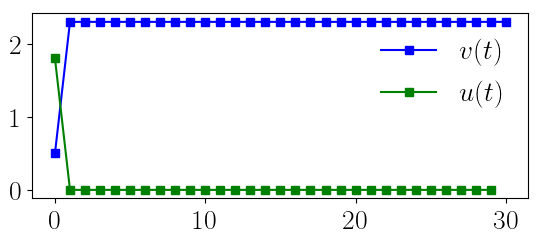
\includegraphics[width=.32\linewidth]{example_6.1_a.png}
    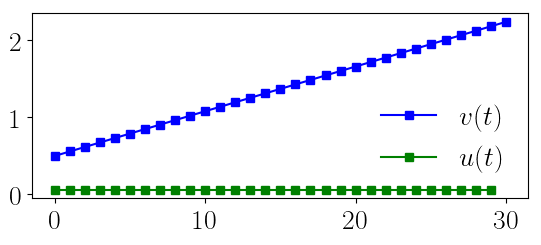
\includegraphics[width=.32\linewidth]{example_6.1_b.png}
    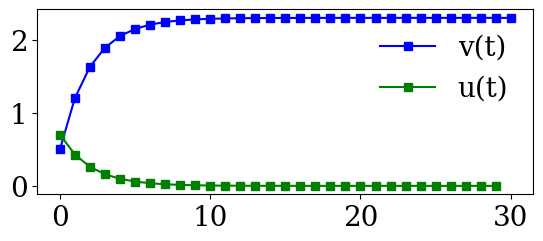
\includegraphics[width=.32\linewidth]{example_6.1_c.png}
    \caption{1D optimal control problem. \textbf{Left:} lowest settling time goal; \textbf{middle:} lowest control signal goal; \textbf{right:} a trade-off between the control signal amplitude and the settling time.}
    \label{fig:lqr}
\end{figure}

Okay, no problem, let us try to penalize large accelerations:
$$
J(\vec{v}, \vec{u}) := \sum\limits_{i=0}^{n-1} u_i^2
$$
Minimization of this criterion is equivalent to solving the following system in the least squares sense:
$$
\left \{ \begin{array}{rl}
u_0     & = 0\\
u_1     & = 0\\
\dots   &    \\
u_{n-1} & = 0\\
\end{array} \right.
$$
Listing~\ref{listing:lqr2} solves this system, and the resulting arrays are shown in the middle image of Figure~\ref{fig:lqr}.
This criterion indeed produces low acceleration, however the transient time becomes unacceptable.

%\inputminted[frame=single,linenos=true]{python}{listings/example_6.1_b.py}

Minimization of the transient time and low acceleration are competing goals, but we can find a trade-off by mixing both goals:
$$
J(\vec{v},\vec{u}) := \sum\limits_{i=1}^n (v_i-v_n)^2 + 4\sum\limits_{i=0}^{n-1} u_i^2 = \sum\limits_{i=1}^n \left(\sum\limits_{j=0}^{i-1}u_j-v_n+v_0\right)^2 + 4\sum\limits_{i=0}^{n-1} u_i^2
$$
This criterion asks to reach the goal as quickly as possible, while penalizing large accelerations. It can be minimized by solving the following system:
$$
\left \{ \begin{array}{ccccl}
u_0 &       &       &           & = v_n - v_0 \\
u_0 & + u_1 &       &           & = v_n - v_0 \\
    &       &       & \vdots    &             \\
u_0 & + u_1 & \dots & + u_{n-1} & = v_n - v_0 \\
2u_0 &        &       &           & = 0 \\
     &  2u_1  &       &           & = 0 \\
     &        &       & \vdots    &     \\
     &        &       &  2u_{n-1} & = 0 \\
\end{array} \right.
$$
Note the coefficient 2 in the equations $2 u_i = 0$ and recall that we solve the system in the least squares sense.
By changing this coefficient, we can attach more importance to one of the competing goals.
Listing~\ref{listing:lqr3} solves this system, and the resulting arrays are shown in the right image of Figure~\ref{fig:lqr}.

%\inputminted[frame=single,linenos=true]{python}{listings/example_6.1_c.py}

Note that the signal $u(t)$ is equal to the signal $v(t)$ up to a multiplication by a constant gain:
$$
u(t) = -F (v(t) - v_{\text{goal}}),
$$
This gain is necessary to know in order to build a closed-loop regulator, and it can be computed from $J$.
In practice, just like we did in this section,
engineers try different combinations of competing goals until they obtain a satisfactory transient time while not exceeding regulation capabilites.






\section{Poisson image editing}
\label{sec:poisson}
The next problem is motivated by image editing.
Figure~\ref{fig:pie} provides an illustration:
we want to replace the baseball from the image \textbf{(a)} with the football \textbf{(b)}. A direct overlay leads to a unsatisfactory result \textbf{(c)}.
How to swap the content seamlessly?

\begin{figure}[tb]
    \centering
    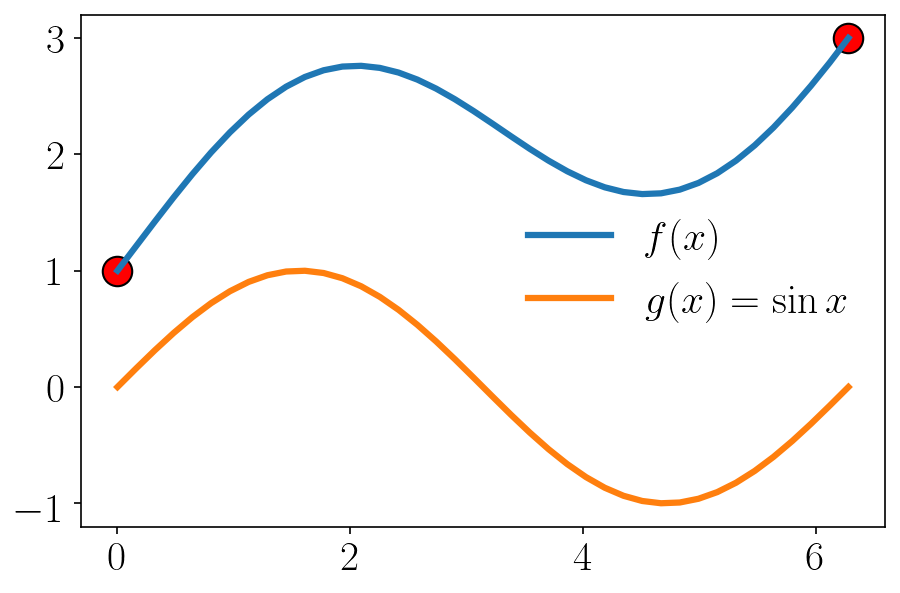
\includegraphics[width=.34\linewidth]{pie-1d.png}
    \caption{1D Poisson's equation: the function $f(x)$ is constrained at the extremities and it has the same second derivative as $g(x)$.}
    \label{fig:pie1d}
\end{figure}

Poisson's equation can be of help here. Let us start with a 1D example from Figure~\ref{fig:pie1d}: we are looking for a unknown function $f(x)$ defined on $x\in[0,2\pi]$ that is as close as possible to $g(x):=\sin x$, but is constrained to have $f(0)=1$ and $f(2\pi) = 3$.
We can formulate it as the Poisson's equation with Dirichlet boundary conditions:
$$
\frac{d^2}{dx^2}f  = \frac{d^2}{dx^2} g \quad \text{s.t.~} f(0)=1,~f(2\pi) = 3
$$

Two decades ago people used Gauß-Seidel to solve these linear systems~\cite{10.1145/882262.882269},
however with modern conjugate gradients-based solvers~\cite{OpenNL} it is much easier to reformulate it as a minimization problem.
Poisson's equation with Dirichlet boundary conditions corresponds to the following least squares formulation:
$$
\min\limits_{f} \int_0^{2\pi} \|f' - g'\|^2 \quad \text{with~} f(0)=1,~f(2\pi) = 3
$$

Let us say that we represent the functions $f$ and $g$ by $n$ samples, then we can obtain $f$ by solving the following linear system in the least squares sense:
\begin{equation}
\label{eq:pie1d}
\left \{ \begin{array}{ccccl}
f_1 &       &       &           & =  g_1 - g_0 + f_0  \\
-f_1 & + f_2 &       &           & = g_2 - g_1 \\
    &       &       & \vdots    &             \\
     &        &  -f_{n-3}     &  f_{n-2}          & = g_{n-2} - g_{n-3} \\
     &        &       & - f_{n-2} & =  g_{n-1}-g_{n-2} -f_{n-1}
\end{array} \right.
\end{equation}
Here we approximate the derivative by finite differences;
this system has $n-1$ equations (one equation per finite difference) with $n-2$ unknowns, $f_0$ and $f_{n-1}$ being fixed.
Listing~\ref{listing:pie1d} solves this system, and the result is shown in  Figure~\ref{fig:pie1d}.

Back to the image editing example (Figure~\ref{fig:pie}). All color channels are solved independently one from another, so we can say that we manipulate grayscale images.
Let us say that we have two real-valued functions $a$ (sub-image of the baseball photo) and $b$ (the football image) defined over $\Omega$.
For the sake of simplicity we consider a rectangular domain $\Omega$.
We are looking for the function $f$ who takes its boundary conditions from $a$ and the gradients from $b$:
$$
\min\limits_{f} \int_\Omega \|\nabla f - \nabla b\|^2 \quad \text{with~} f|_{\partial\Omega} = a|_{\partial\Omega}
$$

\begin{figure}[b]
    \centering
    
\includegraphics[width=.24\linewidth]{pie_baseball.png}~
    \raisebox{0.65\height}{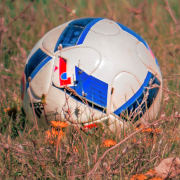
\includegraphics[width=.08\linewidth]{pie_football.png}}~
    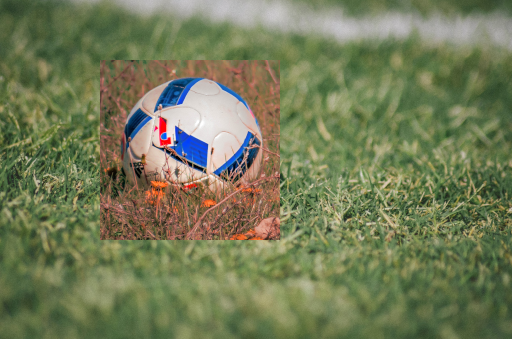
\includegraphics[width=.24\linewidth]{pie_overlay.png}~
    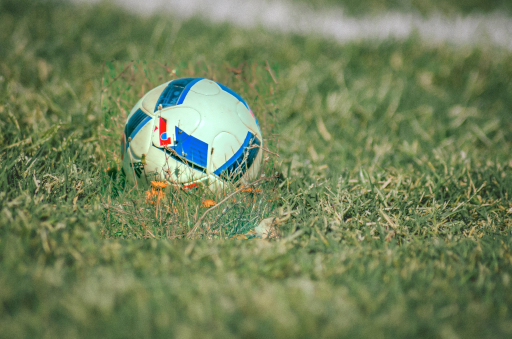
\includegraphics[width=.24\linewidth]{pie_poisson.png}
    \\
    \begin{flushleft}
    {\hspace{.18\linewidth}\textbf{(a)\hspace{.15\linewidth}(b)\hspace{.14\linewidth}(c)\hspace{.22\linewidth}(d)}}
    \end{flushleft}
    \caption{Poisson image editing. We want to replace the baseball from the image \textbf{(a)} with the football \textbf{(b)}. A direct overlay leads to a unsatisfactory result \textbf{(c)}, whereas the Poisson image editing produces an image with much less visible seams \textbf{(d)}.}
    \label{fig:pie}
\end{figure}

We can discretize the problem exactly as in the previous example: if we have $w \times h$-pixels grayscale images $a$ and $b$.
To compute a $w \times h$-pixels image $f$, we can solve the following system in the least squares sense:
\begin{equation}
\label{eq:pie}
\left \{ \begin{array}{rll}
f_{i+1, j}-f_{i,j} & = b_{i+1, j}-b_{i,j} & \forall (i,j) \in [0 \dots w-2] \times [0\dots h-2]\\
f_{i, j+1}-f_{i,j} & = b_{i, j+1}-b_{i,j} & \forall (i,j) \in [0 \dots w-2] \times [0\dots h-2]\\
f_{i,j}            & = a_{i,j}            & \forall (i,j) \text{~s.t.~} i=0 \text{~or~} i=w-1 \text{~or~} j=0 \text{~or~} j=h-1
\end{array} \right.
\end{equation}
Listing~\ref{listing:pie} solves this system, and the result is shown in the rightmost image of Figure~\ref{fig:pie}.



\section{Caricature}
\label{sec:caricature}
Caricature, a type of exaggerated artistic portrait, amplifies the characteristic traits of human faces.
Typically, this task is left to artists, as it has proven difficult for automated methods.
Here we show an extremely naive approach, starting with a 2D silhouette.
This section is closely related to Poisson image editing described in the previous section.
Let us consider the following program:
\inputminted[frame=single,linenos=true]{python}{listings/example_6.2_a.py}

It defines a 2D silhouette as a closed polyline represented by two same length arrays \mintinline{python}{x} and \mintinline{python}{y} (Figure~\ref{fig:lenin-naive}, (a)).
The idea is to increase the curvature of the polyline, thus exaggerating the traits.
To this end, we compute the curvatures via finite differences and store it in the arrays \mintinline{python}{cx} and \mintinline{python}{cy}.
Then we want to solve the Poisson's equation with the increased curvature as the right hand side of the equation.
So, we perform 1000 Gauß-Seidel iterations to solve the equation. Figure~\ref{fig:lenin-naive} shows the evolution of the polyline.
After 10 iterations the drawing looks very good, exactly what we had in mind, but what happens next?
Well, there is no surprise: the polyline is inflated, because it corresponds exactly to what we have asked for.
To scale finite differences is to scale the input signal... How to fix it?
Well, we can stop the process after 10 iterations, thus exploiting the fact that Gauß-Seidel has a slow convergence in low frequencies, but it is a unsatisfactory solution.
It would much be better if the result was at the true minimum of our optimization routine.

\begin{figure}[h]
\begin{minipage}{.66\linewidth}
    \centering
    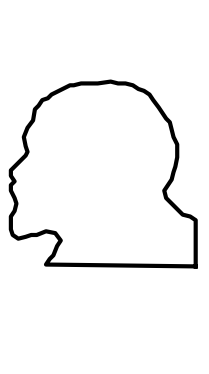
\includegraphics[height=.33\linewidth]{example_6.3_a.png}
    \includegraphics[height=.33\linewidth]{example_6.3_b.png}
    \includegraphics[height=.33\linewidth]{example_6.3_d.png}
    \begin{flushleft}
    {\hspace{.18\linewidth}\textbf{(a)\hspace{.17\linewidth}(b)\hspace{.30\linewidth}(c)}}
    \end{flushleft}
    \caption{Gauß-Seidel iterations amplifying the curvature of the closed polyline shown in image \textbf{(a)}. Image \textbf{(b):} 10 iterations, image \textbf{(c):} 1000 iterations.}
    \label{fig:lenin-naive}
\end{minipage}
\qquad
\begin{minipage}{.25\linewidth}
    \includegraphics[width=\linewidth]{example_6.3_e.png}
    \caption{A trade-off between the desirable curvature and data attachment produces the expected effect.}
    \label{fig:lenin}
\end{minipage}
\end{figure}

The minimization problem that corresponds to the above listing can be written as follows:
\begin{equation}
\label{eq:lenin}
\min \sum\limits_{\forall \text{~edge~} (i,j)} \left(x'_j - x'_i -  c\cdot\left(x_j - x_i\right)  \right)^2,
\end{equation}
where $c$ corresponds to the scaling coefficient, $x_i$ are the input coordinates and $x_i'$ are the unknowns.
The problem is separable in two coordinates, so we list here only the $x$ part.

The simplest way to prevent the ``inflation'' of the model is to add a data attachment term:
\begin{equation}
\label{eq:caricature}
\min \sum\limits_{\forall \text{~edge~} (i,j)} \left(x'_j - x'_i -  c_0\cdot\left(x_j - x_i\right)  \right)^2 + \sum\limits_{\forall \text{~vertex~} i} c_1^2 \left( x'_i - x_i \right)^2
\end{equation}
The coefficients $c_0$ and $c_1$ allow us to tune the optimization to achieve the desired trade-off between the curvature exaggeration and the data attachment.
The result is shown in Figure~\ref{fig:lenin}.
To minimize the energy (Equation~\eqref{eq:caricature}), we can solve the following system in the least squares sense:
\begin{equation}
\label{eq:carsyst}
\left \{ \begin{array}{ccccl}
c_0\cdot x'_0 &            &       &               & =  c_0\cdot x_0  \\
& c_0\cdot x'_1            &       &               & =  c_0\cdot x_1  \\
    &       &       & \vdots    &             \\
&             &       &    c_0\cdot x'_{n-1}           & =  c_0\cdot x_{n-1}  \\
-x'_0 & + x'_1      &       &               & =  c_1\cdot \left( x_1 - x_0\right)  \\
     & - x'_1      & +x'_2      &           & =  c_1 \cdot \left(x_2 - x_1\right)  \\
    &       &       & \vdots    &             \\
    &            & x'_{n-2}   &    +x'_{n-1}       & =  c_1 \cdot \left(x_{n-2} - x_{n-1}\right)  \\
x'_0 &            &    &    -x'_{n-1}       & =  c_1 \cdot \left(x_{n-1} - x_0\right)  \\
\end{array} \right.
\end{equation}
Refer to Listing~\ref{listing:silhouette} for the corresponding source code. Note that we can solve Equation\eqref{eq:caricature} for 3D surfaces as well, an example is shown in Figure~\ref{fig:caricature},
refer to Listing~\ref{listing:caricature} for the source code.

\begin{figure}[ht]
    \centering
    \includegraphics[width=\linewidth]{caricature.jpg}
    \caption{We can solve Equation\eqref{eq:caricature} for 3D surfaces as well (Listing~\ref{listing:caricature}).}
    \label{fig:caricature}
\end{figure}

\newpage
\section{Cubify it!}
\label{sec:cubify}
Let us compute another deformation of a 3D surface, refer to Figure~\ref{fig:moai} for an illustration.
The idea is to deform the surface by aligning triangles with one of the global coordinate planes, thus obtaining a moaï statue effect.
\begin{figure}[!h]
	\centering
	\includegraphics[width=.75\linewidth]{cubify-flagging.jpg}
	\caption{If we flatten an input surface in one of three coordinates (flagging shown in color), we can obtain a moaï statue effect.}
	\label{fig:moai}
\end{figure}

First for each triangle we compute the coordinate axis closest to its normal:
$$
\vec{a}_{ijk} := \argmax\limits_{\vec{u}\in \{(1,0,0), (0,1,0), (0,0,1)\}} \left|\vec{u} \cdot \vec{N}_{ijk}\right| 
$$
Three different colors in the left image of Figure~\ref{fig:moai} correspond to the axes.
And then we want to deform the surface according to this coloring.
It is very easy to do. Let $\vec{e}_{ij}$ denote the vector corresponding to the edge $(i,j)$ in the input data,
and $\vec{e'}_{ij}$ be the modified geometry (the unknowns).
Here is a small test: what would be the result of the following optimization?
$$
\min \sum\limits_{\forall \text{~edge~} ij}\left\|\vec{e'}_{ij} - \vec{e}_{ij}\right\|^2
$$
Surely you have recognized Equation~\eqref{eq:lenin}, it is the simplest Poisson problem, giving the output geometry equal to the input.
We will add few more terms to this energy to obtain the desired effect.

To align the triangles with the coordinate axes, we can define the projection operator by
$$
\text{proj}_{\vec{u}} \vec{v} := \frac{\vec{v}\cdot\vec{v}}{\vec{u}\cdot\vec{u}}\vec{u}
$$
This operator projects the vector $v$ orthogonally onto the line spanned by vector $u$.
Then the desired geometry can be obtained by minimizing the following energy:
\begin{align*}
\min \sum\limits_{\forall \text{~edge~} ij}c_0\left\|\vec{e'}_{ij} - \vec{e}_{ij}\right\|^2 +
\sum\limits_{\forall \text{~triangle~} ijk}c_1\biggl(& \left\|\vec{e'}_{ij} - \vec{e}_{ij} + \text{proj}_{\vec{a}_{ijk}} \left( \vec{e}_{ij}\right) \right\|^2 +\\
&\left\|\vec{e'}_{jk} - \vec{e}_{jk} + \text{proj}_{\vec{a}_{ijk}} \left( \vec{e}_{jk}\right) \right\|^2 +\\
&\left\|\vec{e'}_{ki} - \vec{e}_{ki} + \text{proj}_{\vec{a}_{ijk}} \left( \vec{e}_{ki}\right) \right\|^2\biggr)
\end{align*}
where $c_0$ and $c_1$ represent the trade-off between the flattening and the old data attachment.
Note that $\text{proj}_{\vec{a}_{ijk}} \left( \vec{e}_{ij}\right)$ corresponds to the projection of the vector $\vec{e}_{ij}$ to the plane with the normal vector $\vec{a}_{ijk}$.
Thus, this energy has two types of terms: attachment to the original geometry and the attachment to the triangles projected to one of the coordinate planes.
Listing~\ref{listing:cubify} provides the source code whose result is visible in Figure~\ref{fig:moai}.

\newpage
\section{Least squares conformal mapping}
\label{sec:lscm}
A parameterization of a surface consists in finding a way to store the colors of the surface in a texture.
The mapping of the points of the surface to the texture is defined by a mapping function $\mathbb R^3 \rightarrow \mathbb R^2$.
By inverting this function we can colorize the surface using a flat image drawn by an artist.
Parameterization of a surface is a problem equivalent to flattening this surface.
Figure~\ref{fig:lscm} gives us a pretty intuitive idea of the purpose of parameterization.

\begin{figure}[!h]
	\centering
    \includegraphics[width=.2\linewidth]{lscm-head-mesh.jpg}
    \quad
    \includegraphics[width=.3\linewidth]{lscm-head-uv.jpg}
    \quad
    \includegraphics[width=.2\linewidth]{lscm-head-textured.jpg}
	\caption{Least squares conformal mapping. \textbf{Left:} input mesh; \textbf{middle:} unfolded mesh textured by an artist; \textbf{right:} final textured surface. Two pinned vertices are shown in red.}
	\label{fig:lscm}
\end{figure}


In our context, we are manipulating triangulated surfaces and we define a parametrization as a piecewise linear function where the pieces are the triangles.
Such functions are stored in texture coordinates which are the 2D coordinates of the vertices of the triangulation.

It is very difficult to define what a good parameterization is, there are many different ways to compare the quality of maps.
The distortion of a mapping is defined by the Jacobian matrix.
Ideally, it should be an isometric transformation, but this is an unreachable goal.
In continuous settings, there only exist maps that preserve angles (conformal) and maps that preserve area (authalic).
In this example, we manipulate conformal (angle preserving) maps.

Conformal maps have a very interesting feature:  their distortion is locally reduced to a scaling.
The stretching of the map is the same in all directions (the map is called isotropic), which makes this type of parameterization relatively simple to manipulate.
The conservation of angles implies that the texture (locally) is not elongated.
On the other hand, the area is not conserved, implying eventual strong changes in stretching from one place to another on the surface.

Computing such a mapping~\cite{levy2002least} is a direct instantiation of the Cauchy-Riemann equations on a pair of real-valued functions of two real variables $u(x,y)$ and $v(x,y)$ representing the texture coordinates:
$$\left\{
 \begin{array}{rl}
\frac{\partial u}{\partial x} &= \frac{\partial v}{\partial y} \\
\frac{\partial u}{\partial y} &= -\frac{\partial v}{\partial x}
\end{array}
\right.
$$
%Typically $u$ and $v$ are taken to be the real and imaginary parts respectively of a complex-valued function of a single complex variable $z = x + iy$, $f(x + iy) = u(x,y) + iv(x,y)$.
%Then the Cauchy–Riemann equations may be written in complex form 
%$$
%i\frac{\partial f}{\partial x} = \frac{\partial f}{\partial y}
%$$
In this form, the equations correspond structurally to the condition that the Jacobian matrix is of the form
$ \begin{pmatrix}a & -b \\ b &a\end{pmatrix} $.
Geometrically, such a matrix is always the composition of a rotation with a scaling, and in particular preserves angles.
The Jacobian of a function $(u, v)$ takes infinitesimal line segments at the intersection of two curves in the parameter plane $(x,y)$ and rotates them to the corresponding segments in $u,v$.
Consequently, a function satisfying the Cauchy–Riemann equations, with a nonzero derivative, preserves the angle between curves in the plane.
That is, the Cauchy–Riemann equations are the conditions for a function to be conformal.

Of course, there will be no exact solutions for a triangle mesh, therefore, as usual, we can sum failure of this relationship to hold over all triangles:
$$\min \sum\limits_{\forall\text{~triangle~} ijk} A_{ijk}\left((\nabla u)_{ijk} - N_{ijk}\times(\nabla v)_{ijk}\right)^2,$$
where $A_{ijk}$ is the area of the triangle $ijk$, and $N_{ijk}$ is the normal vector to the triangle. Our maps are linear per triangle, therefore the gradients are constant and can be computed as follows:
$(\nabla u)_{ijk} = \frac{1}{2 A_{ijk}}(u_i \vec{e}_{jk} + u_j\vec{e}_{ki} + u_k\vec{e}_{ij})$.

Of course, we can not do better than $u(x,y)=v(x,y)=0$, and such a map is unsatisfactory. Therefore we can ``pin'' two arbitrary vertices to some arbitrary points in the $u,v$ plane.
Pinning one vertex determines translation in the plane of the texture, whereas the other determines rotation and scale.
This energy is very easy to minimize, just as before we need to solve a linear system.
Refer to Listing~\ref{listing:lscm} for the source code.
This is a very simple program: for each triangle we compute its coordinates in a local 2D basis, compute the expression of $(\nabla u)_{ijk}$ and $(\nabla v)_{ijk}$ in this bais
and create two rows in the matrix (one row per the Cauchy-Riemann equation).
Figure~\ref{fig:lscm} shows the result of the execution of the program.


\section{As-rigid-as possible deformations}
\label{sec:arap}
How to deform a character in a plausible manner?
Usually this task is done by artists expertly rigged 3D models.
However simple deformation models can still produce satisfying deformations~\cite{ARAP_modeling:2007}.
Our deformation will be controlled by a set of vertices $\mathcal{I}$ on the surface which will forced to the position $p_k$ (Figure~\ref{fig:ARAP} left).

\begin{figure}[!h]
 \centering
 \includegraphics[width=\linewidth]{ARAP.jpg}
 \caption{\textbf{Left:} deformation constraints. \textbf{Right:} deformation solution of Equation~\eqref{eq:ARAP}.}
 \label{fig:ARAP}
\end{figure}

The first requirement one might have is that the deformation must be smooth. So the first idea is to best preserve the edge of the original surface as best as possible while satisfying the position constraints. The new vertex positions $x'$ are obtained be solving the least squares problem:
\begin{equation}
 \min_{x'} \sum_{\forall \text{ edge } (i,j)} \left\| x_i' - x_j'- (x_i - x_j) \right\|^2 \quad \text{with } x_k' = p_k , k \in \mathcal{I} .
\label{eq:ARAP_lap}
\end{equation}

The resulting deformation however does not look realistic at all: the surface is badly stretched near the constraints (Figure~\ref{fig:arap-lap}) and the our deformation model is unable to create the global rotation induced by the constraints. How to make the deformation looks like the character is moving? Human(-oid) motions are constraints by a skeleton making any movement a composition of rotations around joints. To simulate this effect we can ask that a vertex neighborhood is the rotation of the vertex neighborhood from the original mesh. This way the deformation will seem more rigid. We assign rotation matrices $R_i$ at each vertex $i$ which will affect all incident edges. The least squares problem has now two sets of unknowns the vertex positions and the rotations:
\begin{equation}
 \min_{x', R} \sum_{\forall \text{ edge } (i,j)} \left\| x_i' - x_j'- R_i (x_i - x_j) \right\|^2 \quad \text{with } x_k' = p_k , k \in \mathcal{I}.
\label{eq:ARAP}
\end{equation}

The problem~\eqref{eq:ARAP} is a nonlinear least squares problem but it can be solved efficiently by alternatively solving for the vertex position and solving for the rotation.
Solving for the vertex positions is a linear problem that can solved by using Gau\ss-Seidel iterations.
Finding the rotations is a so-called \textit{orthogonal Procrustes problem} which has a closed form solution: Let $U \Sigma V^\top$ be the singular value decomposition of the matrix $\sum_{j\text{ incident }i} (x_i' - x_j')(x_i - x_j)^\top$ then $R_i = U V^\top$. 
The resulting deformation is able to create a global rotation of the model while the position constraints  nicely spread out across the surface (Figure~\ref{fig:ARAP} and \ref{fig:arap-lap} right).
Refer to Listing~\ref{listing:arap} for the source code.

\begin{figure}[h]
 \centering
 \includegraphics[width=0.35\linewidth]{arap-lap-a.jpg}
 \includegraphics[width=0.35\linewidth]{arap-lap-b.jpg}
 \caption{\textbf{Left:} the deformation solution of Equation~\eqref{eq:ARAP_lap} is very local and overstretch one finger. \textbf{Right:} the solution of Equation~\eqref{eq:ARAP} creates a local rotation of the hand.}
\label{fig:arap-lap}
\end{figure}



\authoredby{A}
\chapter{Under the hood of the conjugate gradient method}
\fancyhead[R]{\textcolor{blue}{optional for reading}}


The resolution of linear systems is the keystone of a large number of numerical optimization algorithms encountered in many application contexts.
For example, such linear systems play a central role in least-squares-type optimization problems, in
finite-element-based numerical simulation methods as well as in nonlinear function optimization algorithms that solve a series of linear problems.

In this chapter we describe the conjugate gradient method, an algorithm for solving linear systems.
It is widely used because it is very efficient and relatively simple to implement.
It is rather difficult to have a good intuition of its functioning, which we propose to study here.
The conjugate gradient method can very well be used as a black box, but it is more intellectually satisfying to understand how it works.
Moreover, from a practical point of view, this allows to use it in a more efficient way, taking into account the conditioning of the matrix,
by adjusting the number of iterations according to the type of problem, or by programming it in a way to perform all the computations in place
(i.e., without explicitly storing large matrices in memory).

Our approach is to take the point of view of someone looking to reinvent the algorithm.
We will first specify which problem is solved by the method, then we will present two methods of resolution (gradient descent and conjugation),
which can be combined to obtain the conjugate gradient.
We will also illustrate the behaviour of these algorithms under the most common conditions, i.e. with sparse matrices.



\section{Problem statement}

The conjugate gradient method solves the following problem:

\begin{framed}
Given  a symmetric positive definite $n\times n$ matrix $A$ and a vector $b \in {\mathbb R}^n$, find the vector $x \in {\mathbb R}^n$ such that $Ax - b =0$.
\end{framed}

From a geometric point of view, it is quite understandable that to solve a linear system corresponds to calculating the intersection of
the hyperplanes corresponding to each equation (see figure~\ref{fig:pbd2d}).
It is less obvious to understand the conditions on the matrix $A$, and we have dedicated the entire chapter~\ref{sec:mineqlin} to this subject.
In short,
\begin{framed}
%$\nabla (x^\top A x - 2b) = (A+A^\top)x - 2b$; therefore 
Our problem is equivalent to the minimization of the quadratic form $f(x):=x^\top Ax-2b^\top x$. Since $A$ is symmetric positive definite, the solution exists and is unique.
\end{framed}

\begin{figure}[htb]
  \centering
  \includegraphics[width=.8\linewidth]{cg/problem2d.png}
  \caption{Geometric interpretations of the resolution of $Ax-b=0$.
  The dot product of $x$ with each row of $A$ is fixed by $b$.
  Each of these constraints imposes that $x$ is located on a hyperplane (a straight line in 2D, a plane in 3D).
  We can define $x$ as the intersection of these hyperplanes: green and red lines in our 2D example (left) and the three 3D planes (right).
  In the middle, $v=Ax-b$ is shown as a vector field: the solution is the point where the vector field vanishes.
  This field can be seen as  the gradient of a function to be minimized\dots under certain conditions.}
  \label{fig:pbd2d}
\end{figure}


Why reformulating the problem?
Given an invertible $n \times n$ matrix $A$ and an $n$-vector $b$, we would like to solve the matrix equation $Ax = b$.
One way to do so is to invert $A$ and multiply both sides by $A^{-1}$.
While this approach is theoretically valid, there are several problems with it in practice. Computing the inverse of a large
\footnote{It is quite common to manipulate $10^6\times 10^6$ sparse matrices in image and geometry processing.
Recall the Poisson image editing: we want to compute an image, each pixel is a variable of the system. For a rather small $1000\times 1000$ pixels grayscale image we have $10^6$ variables!}
matrix is expensive and susceptible to numerical error due to the finite precision of floating-point numbers.
Moreover, matrices which occur in real problems tend to be sparse and one would hope to take advantage of such structure to reduce
work, but matrix inversion destroys sparsity.
As we will see shortly, iterative methods are the technique of the choice for solving such systems.



\section{Three ways to solve the problem}
\label{chap5:sec:linalg:formulations_pb}

Since we want to perform an unconstrained minimization of a convex function, it is only natural to use an iterative descent method.
In this chapter we study three different methods that share the common structure:
\begin{framed}
\begin{itemize}
\item Make an initial guess $x^{(0)} \leftarrow \vec{0} $;
\item Iterate until convergence:
\begin{itemize}
   \item compute the next step direction $d^{(k)}$;
   \item choose the step size $\alpha^{(k)}$;
   \item update the solution vector $x^{(k+1)} \leftarrow  x^{(k)}+\alpha^{(k)} d^{(k)}$;
\end{itemize}
\end{itemize}
\end{framed}

These three algorithms differ only in the calculation of the step direction. The idea is to start with a very simple method and gradually build the way up to the conjugate gradient method.
So, we start with the famous \textbf{gradient descent (\S\ref{chap5:sec:linalg:descente_gradient})}.
We can minimize the quadratic form $x^\top Ax-2bx$ like any other convex function, however, having a quadratic function allows to calculate an optimal descent step.

Then we present a \textbf{conjugation method (\S\ref{chap5:sec:linalg:algo_conjugaison})}.
This method works not in the original space, but in the space transformed by some linear map $M$, and directly projects the solution on an orthogonal basis.
The vectors whose images by $M$ form an orthogonal base are said to be conjugate (with respect to the scalar product defined by $A$).
This is why this method is called conjugation. \textit{Warning: this method has only a pedagogical interest, it should not be used in practice!}

Finally, we combine two above methods to obtain the \textbf{conjugate gradient method (\S\ref{chap5:sec:linalg:algoGC})}.
The conjugate gradient is a gradient descent in which the directions of descent are modified so that they are conjugated with respect to each other.

\newpage

\section{The 1st way: the gradient descent}
\label{chap5:sec:linalg:descente_gradient}

The gradient of a function gives the direction of fastest increase.
The gradient descent consists of, starting from an initial position $x^{(0)}$,
to move in the direction opposite to the gradient so as to minimize the function as quickly as possible.
Thus, we build a sequence of approximations $x^{(k)}$ that converges to the solution $x^*$.
In the case of a quadratic form, the gradient is easy to compute: $\nabla f(x^{(k)}) = 2Ax^{(k)} - 2b$.
Then the iterative descent method can be instantiated as follows:

\begin{framed}
\begin{itemize}
\setlength\parsep{0pt}
\setlength\itemsep{0pt}
\setlength{\parskip}{0pt}
\setlength{\topsep}{0pt}
\setlength{\partopsep}{0pt}
\item Make an initial guess $x^{(0)} \leftarrow \vec{0} $;
\item Iterate until convergence:
\begin{eqnarray*}
  r^{(k)} &\leftarrow& b -Ax^{(k)}\\
  \alpha^{(k)} &\leftarrow& \frac{r^{(k)\top}r^{(k)}}{r^{(k)\top}Ar^{(k)}}\\
  x^{(k+1)} &\leftarrow& x^{(k)}+\alpha^{(k)} r^{(k)}
\end{eqnarray*}
\end{itemize}
\end{framed}


\subsection{Choosing the step size $\alpha^{(k)}$}
Since we are moving in the opposite direction to the gradient, we are sure to decrease $f$ if we make a sufficiently small step.
That is being said, in our case, we minimize a quadratic form, which, restricted to the search line, remains a quadratic function (a parabola).
It is therefore possible to find directly the optimal step that minimizes $f(x^{(k+1)})$ along the direction $r^{(k)}$.
This can be done by canceling the derivative $\frac{df\left(x^{(k+1)}\right)}{d\alpha^{(k)}}$ with $x^{(k+1)}=x^{(k)}+\alpha^{(k)} r^{(k)}$.

We are looking for $\alpha^{(k)}$ such that $x^{(k)}+\alpha^{(k)} r^{(k)}$ minimizes $f$ along the straight line
generated by the point $x^{(k)}$ and the vector $r^{(k)}$.
To do this, we will cancel the derivative of $f$ along this line:
we want the dot product between the gradient and the search direction to vanish in $x^{(k+1)}$.

Here, the search direction $d^{(k)}$ is equal to the residual $r^{(k)}$, however we keep different notations to preserve the semantics,
which will be useful later on to combine the different approaches.
The step size can be derived from the zero dot product condition as follows:
\begin{eqnarray*}
  d^{(k)\top}r^{(k+1)} &= &0 \\
  d^{(k)\top}\left(b-Ax^{(k+1)}\right) &= &0 \\
  d^{(k)\top}\left(b-A(x^{(k)}+\alpha^{(k)} r^{(k)})\right) &= &0 \\
  \alpha^{(k)}   &=& \frac{d^{(k)\top}\left(Ax^{(k)}-b\right)}{d^{(k)\top}Ar^{(k)}}\\
  \alpha^{(k)} &=& \frac{d^{(k)\top}r^{(k)}}{d^{(k)\top}Ar^{(k)}} 
\end{eqnarray*}

\subsection{Convergence: stopping criterion}
There is no miracle solution. We can stop when the norm of the gradient becomes too small,
or the when the difference $f\left(x^{(k)}\right)-f\left(x^{(k+1)}\right)$ (eventually normalized) is getting too small.

The figures~\ref{fig:gradient2dconverge1} and \ref{fig:gradient3dconverge1} show $2D$ and $3D$ examples of the gradient descent behaviour.
When all eigenvalues of $A$ are equal, the algorithm converges in one iteration, but when they are very different, the speed of convergence drastically decreases.
The maximum ratio between the eigenvalues is called the matrix conditioning, and reflects well the difficulty of the problem.

\begin{figure}[p]
  \centering
  \includegraphics[width=1\linewidth]{cg/gradient2Dconverge.png}
  \caption{
Optimal step gradient descent with a diagonal matrix $A$, where $a_{00}$ takes values from 1 (left) to 5 (right), $a_{11}=1$ and $a_{10}=a_{01}=0$.
The blue segments connect the $x^{(k)}$ to the $x^{(k+1)}$, and the ellipses show the iso-values of $f(x)=x^\top Ax-2b^\top x$.
}
  \label{fig:gradient2dconverge1}

  \includegraphics[width=1\linewidth]{cg/gradient3Dconverge1.png}
  \caption{
  A 3D example of gradient descent with a diagonal matrix $A$. We observe an extremely fast convergence when $A$ is close to the identity (left), 
  and a particularly slow convergence when its diagonal elements are $0.5,1$ and $2$ (right). }
  \label{fig:gradient3dconverge1}

  \includegraphics[width = \linewidth]{cg/defpositiveness.png}
  \caption{
Few 2D linear maps transforming an image.
From left to right: the identity matrix does not change the image, more generally, a diagonal matrix stretches the image along the coordinate axes.
Even more generally, all symmetric positive definite define a stretch along orthogonal directions.
Antisymmetric matrix flips axes (negative coefficient stretching),
and a rotation matrix  ``stretches'' with a complex coefficient.}
  \label{fig:eigenSPD}

\end{figure}

\vspace{10mm}

To sum up, \textit{the gradient descent is a very simple method, and has a very fast convergence rate during first iterations.
After few iterations, its behaviour becomes very sensitive to the matrix conditioning.}


\section{The 2nd way: the (naïve) conjuguation method}
\label{chap5:sec:linalg:algo_conjugaison}

Let us put aside the minimization for a moment, and cosider a projection method that solves $Ax=b$ directly.
The idea is to build an orthogonal basis and project the solution onto this basis in $n$ iterations.
Before doing so, let us build few handy tools first.

\subsection{A very useful linear map $M=\sqrt{A}$}
In this method a central role is played by the map $M$ that we can loosely describe as $M:=\sqrt{A}$.
The idea is to make orthogonal projections in the space transformed by the map $M$.

\begin{framed}
We define $M$ as a symmetric matrix having the same eigenvectors as $A$ but whose eigenvalues are the square roots of those of $A$.
This matrix is symmetric positive definite with real entries.
\end{framed}
The (slightly abusive) notation $M := \sqrt{A}$ comes from the fact that $M^\top M=MM=A$ as you can see:

\begin{itemize}
\item either via a \textit{geometrical intuiton}: as we will see shortly, $A$ has a full set of real-valued eigenvectors forming an orthonormal basis $\{v_i\}_{i=1}^{n}$.
We can decompose any vector $x$ in this basis, therefore $Ax = \sum_{i=1}^{n} (x^\top v_i) \lambda_i v_i$.
This means that the linear map defined by $A$ is simply a stretching of space in the directions of each eigenvector, with a factor given by the associated eigenvalue (Figure~\ref{fig:eigenSPD}).

Than the linear map $M$ can be seen as two consequtive stretchings of space along the same vectors, but with corresponding factors $\sqrt{\lambda_i}$.
This is equivalent to stretching by $\lambda_i$ (Figure~\ref{fig:stretchM}).

\item either \textit{analytically:} since $A$ is symmetric positive definite, it has a full set of real-valued eigenvectors forming an orthonormal basis.
Let $v_i$ and $v_j$ be two eigenvectors associated with distinct eigenvalues $\lambda_i \neq \lambda_j$: $Av_i=\lambda_iv_i$ and $Av_j=\lambda_jv_j$.
The symmetry of $A$ implies that:
\begin{align*}
  v_i^\top A v_j & =  v_j^\top A v_i \\
  v_i^\top \lambda_j v_j & =  v_j^\top \lambda_i v_i \\
  (\lambda_j -\lambda_i) \left(v_i^\top v_j\right)& =  0.
\end{align*}
Thus, if $v_1$ and $v_2$ correspond to two distinct eigenvalues, they are orthogonal.
Even if there is an infinity of eigenvectors (due to multiple eigenvalues), it can be shown that $A$ has a full orthonormal basis of eigenvectors.

Then let us examine the action of $M$:
$$
M^\top Mx =MMx = \sum_{i=1}^{n}\sum_{j=1}^{n}\sqrt{\lambda_i}\left(\sqrt{\lambda_j} x^\top v_j\right) v_i = \sum_{i=1}^{n} \lambda_i v_i \left(x^\top v_i\right) = Ax.
$$
Moreover, as $A$ is positive definite, it means that $x^\top Ax>0, \forall x \neq 0$.
In particular, for an eigenvector $v$ with associated eigenvalue $\lambda$ (i.e., $Av=\lambda v$), 
we have $v^\top \lambda v > 0$. This implies that $\lambda>0$ (and, by the same token, that $\lambda \in \mathbb{R}$). 
Therefore, all eigenvalues of $A$ are real and positive, and the square roots are well-defined.
\end{itemize}

\begin{figure}[p]
\centering
  \includegraphics[width=1\linewidth]{cg/MMA.png}
  \caption{
The linear map $A$ can be seen as a repeated action of $M$.
The eigenvectors (orange and white arrows) of $A$ and $M$ are the same: only the eigenvalues are different (squared).}
  \label{fig:stretchM}

  \includegraphics[width=.8\linewidth]{cg/Aorth.png}
  \caption{Let $u$ and $v$ be two arbitrary vectors and $x^*$ the solution of $Ax-b=0$.
  We can easily calculate dot products $Mu\cdot Mv$ and $Mu\cdot Mx^*$.
  This makes it possible to project $v$ and $x^*$ onto $u$ in a way that would be orthogonal in $M$.}
  \label{fig:Aorth}

  \includegraphics[width=.7\linewidth]{cg/proj2D.png}
  \caption{The conjuguation method in 2D. We start from two arbitrary linearly independent vectors $r^{(0)}$ and $r^{(1)}$, and then we define $d^{(0)} \leftarrow r^{(0)}$
    and $d^{(1)} \leftarrow M^{-1}\left(Mr^{(1)}-proj\left(Mr^{(1)}/Md^{(0)}\right)\right)$. 
    Note that $d^{(0)}$ and $d^{(1)}$ form an $A$-orthogonal basis.
    Then the solution $x^*$ can be decomposed in this basis as
    $x^*\leftarrow \Sigma_k M^{-1}proj\left(Mx^*/Md^{(k)}\right)$.}
  \label{fig:proj2D}

\end{figure}


\subsection{$A$-orthogonality}

Note that although we define $M$, we never compute it explicitly.
The interest of defining $M$ is that one can easily compute dot products in the space transformed by $M$.
Indeed, if we want to calculate the dot product between the images of two vectors $u$ and $v$ under the map $M$,
we need to evaluate $(Mu)^\top Mv = u^\top Mv = u^\top Av$.
Note that it can be done without having $M$ computed! As a side note, $A$ defines the metric tensor of the linear map associated with $M$:
it is a bilinear map that allows to measure the dot product (thus lengths and angles) in the space transformed by $M$.


So, we can very efficiently compute $(Mu)^\top Mv = u^\top Av$, the dot product of $Mu$ and $Mv$, images of any two vectors $u$ and $v$.
It is therefore very easy to know whether $Mu$ and $Mv$ are orthogonal ($u^\top Av = $0).
Moreover, it is also simple to compute the norm of a transformed vector: $\|Mu\|=\sqrt{u^\top Au}$.
\textbf{Note that even if we do not know the true soluton $x^* := A^{-1}b$, we can efficiently compute $(Mu)^\top Mx^* = u^\top b$ for any vector $u$,}
and this is the key property for recovering the solution itself.


\begin{framed}
In practice, we will use the above properties to build an $A$-orthogonal basis: for any two vectors $u$ and $v$ from this basis, $Mu \perp Mv$.
This basis will help us greatly, since we know to project easily the (unknown) solution $x^*$ onto the basis (Figure~\ref{fig:Aorth}).
\end{framed}

\subsection{Back to the naïve conjuguation method}
Recall that we have put aside for a moment the minimization of $x^\top A x - 2b^\top x$,
and the goal is to build a direct way to solve for $Ax=b$.

We want to build an orthogonal basis and project the solution onto this basis, what can be done in $n$ iterations.
To do so, we start from an arbitrary set of linearly independent vectors $\left\{r^{(k)}\right\}_{k=0}^{n-1}$
and use a variant of the Gram-Schmidt process to build a set of $A$-orthogonal vectors $\left\{d^{(k)}\right\}_{k=0}^{n-1}$.
It can be thought as the ordinary Gram-Schmidt normalization of the set $\left\{Mr^{(k)}\right\}_{k=0}^{n-1}$ that builds an orthogonal set $\left\{Md^{(k)}\right\}_{k=0}^{n-1}$.
Recall that we never actually compute $M$; we find it easier to reason in terms of an orthogonal basis rather than manipulate $A$-orthogonality,
even if we do actually build an $A$-orthogonal basis $\left\{d^{(k)}\right\}_{k=0}^{n-1}$.
Finally, we compute an orthogonal projection of $Mx^*$ onto $\left\{Md^{(k)}\right\}_{k=0}^{n-1}$ and, by the linearity of $M$, we deduce the contribution of every $d^{(k)}$ to $x^*$.

So, we need to \textbf{(1)} construct the basis and \textbf{(2)} project the solution onto it:
\begin{enumerate}
\item \textbf{Basis construction.}
Let us take any set of $n$ linearly independent vectors $\left\{r^{(k)}\right\}_{k=0}^{n-1}$, for example: 
$$r^{(k)}_i=\left\{
  \begin{array}{ll}
    1 & \mbox{si } i=k\\
    0 & \mbox{si } i\neq k \\
  \end{array}
  \right.$$

Since $M$ is (strictly) positive definite, $\left\{Mr^{(k)}\right\}_{k=0}^{n-1}$ are also linearly independent.

Gram-Schmidt process builds the set incrementally, and only needs to know how to evaluate dot products.
Geometrically, this method proceeds as follows: first we define $d^{(0)}:=r^{(0)}$ (and thus $Md^{(0)}=Mr^{(0)}$).
and then to compute $Md^{(k)}$, first it projects orthogonally $Mr^{(k)}$ onto the subspace $\Span\left\{Md^{(0)}\dots Md^{(k-1)}\right\}$.
The vector $Md^{(k)}$ is then defined to be the difference between $Mr^{(k)}$ and this projection, guaranteed to be orthogonal to all of the vectors in the above subspace.

Refer to Figure~\ref{fig:Aorth} for an illustration;
recall that the projection of a vector $v$ onto the system axis represented by the vector $u$
is the vector $u$ scaled by the factor $v \cos(\angle(u,v))$.
We can find it by computing two dot products:  $proj(v,u) := \frac{u^\top v}{u^\top u}u$.
Here, we use this equation with $v = Mr^{(k+1)}$ and $u=Md^{(i)}$
in order to project the new direction onto the preceding ones and thus decompose 
$Mr^{(k+1)}$ into $Md^{(0)}\dots Md^{(k)}$.

\begin{align*}
  Md^{(k+1)} =&Mr^{(k+1)} - \sum_{i=0}^k \frac{\left(Mr^{(k+1)}\right)^\top Md^{(i)}}{\left(Md^{(i)}\right)^\top Md^{(i)}} Md^{(i)}\\ 
  =& Mr^{(k+1)} - \sum_{i=0}^k \frac{r^{(k+1)\top}Ad^{(i)}}{d^{(i)\top}Ad^{(i)}} Md^{(i)}
\end{align*}

This relation is interesting, however our real uknowns are $d^{(k)}$ and not $Md^{(k)}$. So, we multiply both parts of the equation by $M^{-1}$ (ref. to Figure~\ref{fig:Aorth}):
\begin{equation}
  \label{eq:naive_gram_update}
  d^{(k+1)} \leftarrow r^{(k+1)} - \sum_{i=0}^k \frac{r^{(k+1)\top}Ad^{(i)}}{d^{(i)\top}Ad^{(i)}} d^{(i)}.
\end{equation}
This is the formula that will be used in the algorithm because it
no longer contains the matrix $M$ we don't know, but only $A$ and the previous vectors $d^{(0)}\dots d^{(k)}$.

\item {\bf Projection of $Mx^*$ onto this basis.}
As before, two dot products allow us to find projection on each of the vectors:
\begin{align*}
  Mx^* =& \sum_{k=0}^{n-1} \frac{(Mx^*)^\top Md^{(k)}}{(Md^{(k)})^\top Md^{(k)}} Md^{(k)}\\
    =& \sum_{k=0}^{n-1} \frac{x^*Ad^{(k)}}{d^{(k)\top}Ad^{(k)}} Md^{(k)} \\
  =& \sum_{k=0}^{n-1} \frac{b^\top d^{(k)}}{d^{(k)\top}Ad^{(k)}} Md^{(k)}. 
\end{align*}

Again, we can't do this calculation since we don't know $M$, but we can find $x^*$ directly by multiplying the formula on either side by $M^{-1}$:
$$
x^* \leftarrow \sum_{k=0}^{n-1} \frac{b^\top d^{(k)}}{d^{(k)\top}Ad^{(k)}} d^{(k)}.
$$
\end{enumerate}

Note that we do need to calculate the full set $\left\{d^{(k)}\right\}_{k=0}^{n-1}$ prior projecting $Mx^*$ onto the $Md^{(k)}$.
To make the conjugation algorithm closer to the conjugate gradient algorithm, we regroup the two loops into the single one;
then the algorithm can be written as follows:
\begin{framed}
\begin{itemize}
\item $d^{(0)}\leftarrow r^{(0)}$
\item $x^{(0)} \leftarrow \vec{0} + \frac{b^\top d^{(0)}}{d^{(0)\top}Ad^{(0)}} d^{(0)}$
\item for $k \in 1\dots n-2$:
\begin{itemize}
    \item $d^{(k+1)} \leftarrow r^{(k+1)} - \sum_{i=0}^k \frac{r^{(k+1)\top}Ad^{(i)}}{d^{(i)\top}Ad^{(i)}} d^{(i)}$
    \item $x^{(k+1)} \leftarrow x^{(k)} + \frac{b^\top d^{(k)}}{d^{(k)\top}Ad^{(k)}} d^{(k)}$
\end{itemize}
\end{itemize}
\end{framed}


To sum up, we can solve $Ax=b$ by building an orthogonal base in $M$ and projecting the image of the solution on it just by computing dot products in $M$.
Figure~\ref{fig:proj2D} provides an illustration.

This algorithm has a $O(n^3)$ complexity because of the necessity to reiterate Gram-Schmidt every time when we choose a new direction, which is regrettable.
This algorithm should not be implemented because it is very inefficient.
It forms, however a perfect basement for the conjugate gradient method.

\newpage
\section{The 3rd and final algorithm: the conjugate gradient}
\label{chap5:sec:linalg:algoGC}

The conjugate gradient differs from the previous algorithm in the way it constructs the $r^{(k)}$.
Instead of taking an arbitrary basis, we define it to be the residual at each iteration $r^{(k)} = b-Ax^{(k)}$.
Recall that the gradient of the corresponding quadratic form is collinear with the residual, hence the name:
$$\nabla\left\{x^\top A x + 2b^\top x\right\}\left(x^{(k)}\right) = -2 r^{(k)}.$$
In this way, we combine the gradient descent and the naïve conjugation to obtain the conjugate gradient method.
This choice of $r^{(k)}$ offers two advantages: it cancels most of the terms in the equation~\eqref{eq:naive_gram_update} and allows the algorithm to converge numerically long before reaching the $n$-th iteration.
So, while the conjuguate gradient algorithm can be seen as a direct solving method (if $n$ iterations are performed),
the most important contributions are made in the beginning, therefore it can also be seen as an iterative method.

We can rewrite the naïve conjuguation algorithm as follows:

\begin{center}
\begin{tabular}{|c|l|l|}
  \hline
line &  Direct adaptation & Optimized adaptation  \\
  \hline
1&  $x^{(0)}\leftarrow 0$ &$x^{(0)}\leftarrow 0$ \\
2&  $r^{(0)}\leftarrow b - Ax^{(0)}$ & $r^{(0)}\leftarrow b - Ax^{(0)}$ \\
3&  $d^{(0)}\leftarrow r^{(0)}$ & $d^{(0)}\leftarrow r^{(0)}$\\
4&  For $k\in 0\dots n-1$: & For $k\in 0\dots n-1$:  \\
5&  \quad $\alpha^{(k)} \leftarrow   \frac{b^\top d^{(k)}}{d^{(k)\top}Ad^{(k)}} $                   & \quad $\alpha^{(k)} \leftarrow   \frac{r^{(k)\top} r^{(k)}}{d^{(k)\top}Ad^{(k)}} $\\
6&  \quad $x^{(k+1)} \leftarrow x^{(k)}+\alpha^{(k)} d^{(k)} $                                      & \quad $x^{(k+1)} \leftarrow x^{(k)}+\alpha^{(k)} d^{(k)} $\\
7&  \quad $r^{(k+1)} \leftarrow b-Ax^{(k+1)}$                                                       & \quad $r^{(k+1)} \leftarrow r^{(k)}-\alpha^{(k)} Ad^{(k)} $\\
8&  \quad $\beta^{(k+1)}_i \leftarrow \frac{r^{(k+1)\top}Ad^{(i)}}{d^{(i)\top}Ad^{(i)}}, \forall i\leq k$ & \quad $\beta^{(k+1)} \leftarrow - \frac{r^{(k+1)\top} r^{(k+1)}}{r^{(k)\top} r^{(k)}}$ \\
9&  \quad $d^{(k+1)} \leftarrow r^{(k+1)} - \sum_{i=0}^{k}\beta^{(k+1)}_id^{(k)}$                   & \quad $d^{(k+1)} \leftarrow r^{(k+1)} - \beta^{(k+1)}d^{(k)}$\\
  \hline
\end{tabular}
\end{center}

The right column presents an optimized version of the algorithm that we will describe in details shortly.
Note the drastic change in complexity: the performance-killing sum in the last line disappears in the optimization!
While the left column is quite straightforward to obtain, the optimized version requires a little bit more analysis.
The most striking property allowing us to perform this optimization is the orthogonality of the residuals:
$$
\boxed{{r^{(k)}}^\top r^{(i)}=0 \quad \forall k<i}
$$
It is easy to prove: recall that once we take a step in a search direction, we need never step in that direction again, i.e.
$\left(Mx^{(k)} - Mx^*\right) \perp \Span\left\{Md^{(0)}, \dots Md^{(k-1)}\right\}$, it means that the error $x^{(k)} - x^*$ is $A$-orthogonal to the subspace $D^{(k-1)}:=\Span\left\{d^{(0)}, \dots d^{(k-1)}\right\}$.
Since the residual $r^{(k)} = A\left(x^*-x^{(k)}\right)$, then $r^{(k)}$ is orthogonal to $D^{(k-1)}$.
Let us note that $D^{(k-1)} = \Span\left\{r^{(0)}, \dots r^{(k-1)}\right\}$, it can be easily demonstrated by induction using the fact that $d^{(j)}$ is
a linear combination of $r^{(j)}$ and $d^{(i)}$ with $i<j$.
We can conclude then that the set of residuals $\left\{r^{(k)}\right\}_{k=0}^{n-1}$ form an orthogonal basis,
and it is conjugated to the basis $\left\{d^{(k)}\right\}_{k=0}^{n-1}$, who, in its turn, becomes orthogonal under the action of $M$, refer to Figure~\ref{fig:conjuge} for an illustration.

\begin{figure}[t]
  \centering
  \includegraphics[width=1\linewidth]{cg/conjuge.png}
  \caption{The vectors $\left\{r^{(k)}\right\}_{k=0}^{n-1}$ (in red) are mutually orthogonal, as well as
  the vectors $\left\{Md^{(k)}\right\}_{k=0}^{n-1}$ (in blue) are mutually orthogonal in the space deformed by $M$.}
  \label{fig:conjuge}
\end{figure}


Armed with this key property, let us review all the transformations leading to the optimized version of the algorithm:
\begin{itemize}
\item \textbf{Line 5: step size $\alpha^{(k)}$.} The optimal step size can be computed both via the conjuguation and the gradient descent:
$$\boxed{\alpha^{(k)}=\frac{r^{(k)\top}r^{(k)}}{d^{(k)\top}Ar^{(k)}} =\frac{b^\top d^{(k)}}{d^{(k)\top}Ad^{(k)}}}$$

We compute the step $\alpha^{(k)}$ so that the gradient at the new point is orthogonal to the search direction.
For the gradient descent we look for $d^{(k)}\perp r^{(k+1)}$, and for the conjugation method we look for $Md^{(k)}\perp Mr^{(k+1)}$.
Since placing $x^{(k+1)}$ at the minimum of $\|Ax-b\|^2$ is equivalent to placing $Mx^{(k+1)}$ at the minimum of $\|Ax-b\|^2$ transformed by $M$, 
we obtain the same $\alpha^{(k)}$ in both cases.

It is easy to see that $d^{(k)\top}Ar^{(k)} = d^{(k)\top}Ad^{(k)}$:
to construct $Md^{(k)}$ with Gram-Schmidt, a vector of $MD^{(k-1)}$ was subtracted from $Mr^{(k)}$, leaving the same the dot product with $Md^{(k)}$.
We have therefore the equailty of the denominators.
Knowing that $x^{(k)}\in D^{(k-1)}$, we also determine the equality of the numerators: 
$ b^\top d^{(k)} =(b-Ax^{(k)})^\top d^{(k)} = r^{(k)\top}d^{(k)}=r^{(k)\top}r^{(k)}$.
The last equality comes from the fact that the residuals are mutually orthogonal.
More presicely, to find $d^{(k)}$ with aid of the Gram-Schmidt process, we have subtracted a vector lying in $D^{(k-1)}$ from $r^{(k)}$;
keeping in mind that $r^{(k)}\perp D^{(k-1)}$, it therefore does not modify the dot product $r^{(k)\top} r^{(k)}$, leaving it equal to $d^{(k)\top} r^{(k)}$.

\item \textbf{Line 7: recursive definition of $r^{(k)}$.} \fbox{$r^{(k+1)}= r^{(k)}+\alpha^{(k)} A d^{(k)}$}

By definition $r^{(k+1)} = b-Ax^{(k+1)}$. We know that $x^{(k+1)} = x^{(k)}+\alpha^{(k)} d^{(k)}$, thus $r^{(k+1)} = b-A(x_i+\alpha^{(k)} d^{(k)}) = r^{(k)} + \alpha^{(k)} A d^{(k)}$.

\item \textbf{Lines 8 and 9: massive cancellation of betas.}
The first two simplifications are simple and only slightly affect performance.
The last simplification is fundamental because it changes each iteration in $O(n)$ instead of $O(n^2)$ (with sparse matrices):
it uses the orthogonality of the residuals to simplify the writing of $\beta^{(k+1)}_j$.

By definition of betas, we have:
\begin{align*}
  \beta^{(k+1)}_i&:= \frac{r^{(k+1)\top}Ad^{(i)}  }{d^{(i)\top}Ad^{(i)}} \\
&= \frac{r^{(k+1)\top}(r^{(i)}- r^{(i+1)})  }{\alpha^{(i)} d^{(i)\top}Ad^{(i)}} \\
  &= \frac{r^{(k+1)\top}r^{(i)}- r^{(k+1)\top}r^{(i+1)}}{\alpha^{(i)} d^{(i)\top}Ad^{(i)}},
\end{align*}
where the first transformation is made thanks to the recursive definition of the residuals $r^{(i+1)}= r^{(i)}+\alpha^{(i)} A d^{(i)}$.
Then, by orthogonality of the residuals, we have:

\begin{equation}
\nonumber
\boxed{
\begin{array}{rcl}
\beta^{(k+1)}_i &= \left \{ \begin{array}{r l} \frac{- r^{(k+1)\top}r^{(k+1)}}{\alpha^{(k)} d^{(k)\top}Ad^{(k)}}, & i=k\\ 0, & i<k \end{array} \right. \\
                &= \left \{ \begin{array}{r l} \frac{- r^{(k+1)\top}r^{(k+1)}}{r^{(k)\top}r^{(k)}}, & i=k\\ 0, & i<k \end{array} \right. 
\end{array}
}
\end{equation}
The last transformation was obtained by plugging the optimized definition of $\alpha^{(k)}$ into the right-hand side of the equation.

To sum up, by orthogonality of the residuals, $\beta^{(k+1)}_i=0$ if $k\neq i$, which makes it possible to simplify the notations by omitting the $i$:
we use $\beta^{(k+1)}$ instead of $\beta_k^{(k+1)}$ because all the other $\beta_i^{(k+1)}$ are null.

\end{itemize}


\newpage
\section{Performance}

In the absence of rounding errors, the conjugate gradient converges in $n$ iterations; each iteration requires only one matrix-vector multiplication of five dot products.
In practice, the conjugate gradient is used on large sparse matrices as an iterative solver that is less sensitive to matrix conditioning than the gradient descent.

It is interesting to observe the behaviour of the conjugate gradient on this type of matrices.
In this section we present two simple cases: a 1D Laplacian and a 2D Laplacian discretized on a regular grid.
Although simple, these choices show the impact of a predominant factor for the solvers behaviour: the arrangement of zeros in the matrix, which corresponds to the geometric neighborhoods in the discretized space.

The sparse matrices define graphs that link the indices~$i$ and~$j$ by non-zero matrix entries $a_{ij}$.
In finite element modeling (FEM) and in geometry processing, these graphs are very close to the structure of the underlying mesh.
Indeed, by their definition, derivatives are estimated on neighbouring elements.
These two example allow us to see how the algorithms we have just presented behave with this type of data.

\subsection{1D Laplacian}

We represent a function~$f$ by the vector~$x$ such that $f(i) = x_i$.
We can estimate its second derivative by finite differences;
the problem is to find a function (the vector $x$) whose second derivative is null, and which respects boundary constraints shown in Figure~\ref{fig:laplace1d}.

This problem is very interesting because it is relatively simple to analyze.
In addition, we can visualize the behavior of the various algorithms on a single image (Figure~\ref{fig:laplace1dresults}): we display $x_i^{(k)}$ as a function of the position $i$ and iteration $k$.
Moreover, this problem is extremely complex to solve because the conditioning of the system is very bad: for $n=5$ it is $13.6= 1.9 / 0.14$ and for $n=20$, it's equal to $200 = 2/.01$.
Geometrically, this corresponds to minimizing a quadratic function $x^\top Ax-2b^\top x$ whose iso-values are ellipses with aspect ratios of 13.6 and 200!


For each algorithm, we observe following behaviour (Figure~\ref{fig:laplace1dresults}):
\begin{itemize}
\item Gradient descent quickly minimizes the second derivative near the constraints, but struggles to propagate the constraints into the domain.
\item The projection method propagates the left-hand constraint as it goes along, but does not take into account the right-hand constraint until the very last iteration.
This behavior is certainly due to the choice of $r^{(k)}$, but illustrates the necessity to perform all $n$ iterations.
\item The conjugate gradient behaves as if it only sees a small region around the constraints (shown in orange at the edges), where it perfectly solves the problem.
This region grows at each iteration to cover the whole domain at $n/2$ iterations, but it is necessary to wait for all the $n$ iterations before each of the two constraints has had time to influence the whole domain.
\end{itemize}

\begin{figure}[p]
  \centering
  \includegraphics[width=1\linewidth]{cg/laplace1d.png}
  \caption{1D Laplacian problem. We have a function defined in $n=5$ points; the goal is to minimize the second derivative estimated by finite differences i.e., $\Sigma_i( x_i-(x_{i-1}+x_{i+1})/2)$. 
    At the boundary we fix values $h_0$ and $h_n$, which gives the problem $Ax-b=0$ with $A$ and $b$ shown in the figure. }
  \label{fig:laplace1d}
  \vspace{5mm}

  \includegraphics[width=1\linewidth]{cg/laplace1dresults.png}
  \caption{
    Evolution of the solution with $n=20$: the gray axis represents the function sampled by $x$, and the blue axis is the iteration axis, the orange segments are the boundary constraints.
  Three solvers are (from left to right) the gradient descent, the conjugation and the conjugated gradient.
  }
  \label{fig:laplace1dresults}
  \vspace{5mm}

  \includegraphics[width=1\linewidth]{cg/laplace2d.png}
  \caption{
    Evolution of the 2D Laplacian solution on a $20\times 20$ grid.
  The solution $x$ is displayed by the height of the function, and the boundary constraints are given by the orange segments.
  }
  \label{fig:laplace2d}
\end{figure}

\subsection{2D Laplacian}

The 2D Laplacian works on the same principle as the 1D Laplacian.
We have discretized a function $f$ on a 2D grid and each entry of the vector $x$ is associated with each node of the grid.
The Laplacian is estimated by finite difference, so the matrix $A$ is defined by: $a_{ii}=1$, $a_{ij}=-1/4$ if the nodes $i$ and $j$ are neighbors, and $a_{ij}=0$ otherwise.

In the 2D case, we can no longer represent the simulation on a single image, so we display the state at certain iterations.
Thanks to the Figure~\ref{fig:laplace2d}, we can analyze the behavior of the algorithms:
\begin{itemize}
\item
Gradient descent: like with 1D Laplacian, we observe that the first iterations smooth out the function well, but that the solver struggles to propagate the constraints towards the interior of the domain.
This being said, in 100 iterations, the convergence on this $20\times 20$ grid seems similar to that observed on the 1D grid of $n=20$.
The difficulty does not seem to be due to 400 variables, but rather to the distance to the constraints (which is about the same in 1D and 2D).
\item Conjugation: the solver has set the $x_i$ one after the other, and did not converge because we stopped it before the necessary 400 iterations.
\item Conjugate gradient: it converges in less than 30 iterations, which is far from the 400 iterations necessary (direct method) to guarantee convergence.
This behavior can be explained by the time needed for each constraint to influence the whole domain.
\end{itemize}


%	inputs for http://www.bluebit.gr/matrix-calculator/calculate.aspx
%	-1  .5 0 0 0   
%	.5  -1 .5 0 0   
%	0 .5 -1 .5  0 
%	0 0  .5 -1 .5 
%	0 0  0 .5 -1 
%	
%	 -1  .5 0 0 0   0 0 0 0 0    0 0 0 0 0    0 0 0 0 0  
%	.5  -1 .5 0 0   0 0 0 0 0    0 0 0 0 0    0 0 0 0 0 
%	0 .5 -1 .5  0   0 0 0 0 0    0 0 0 0 0    0 0 0 0 0 
%	0 0  .5 -1 .5   0 0 0 0 0    0 0 0 0 0    0 0 0 0 0 
%	0 0 0 .5 -1    .5 0 0 0 0      0 0 0 0 0   0 0 0 0 0
%	0 0 0 0 .5    -1 .5 0 0 0    0 0 0 0 0   0 0 0 0 0
%	0 0 0 0 0    .5 -1 .5 0 0      0 0 0 0 0   0 0 0 0 0
%	0 0 0 0 0    0 .5 -1 .5 0   0 0 0 0 0   0 0 0 0 0
%	0 0 0 0 0    0 0 .5 -1 .5    0 0 0 0 0   0 0 0 0 0
%	0 0 0 0 0    0 0 0 .5 -1    .5 0 0 0 0    0 0 0 0 0
%	0 0 0 0 0   0 0 0 0 .5    -1 .5 0 0 0    0 0 0 0 0
%	0 0 0 0 0   0 0 0 0 0    .5 -1 .5 0 0      0 0 0 0 0
%	0 0 0 0 0   0 0 0 0 0    0 .5 -1 .5 0   0 0 0 0 0
%	0 0 0 0 0   0 0 0 0 0    0 0 .5 -1 .5    0 0 0 0 0
%	0 0 0 0 0   0 0 0 0 0    0 0 0 .5 -1    .5 0 0 0 0 
%	0 0 0 0 0   0 0 0 0 0    0 0 0 0 .5    -1 .5 0 0 0 
%	0 0 0 0 0   0 0 0 0 0   0 0 0 0 0    .5 -1 .5 0 0   
%	0 0 0 0 0   0 0 0 0 0   0 0 0 0 0    0 .5 -1 .5 0
%	0 0 0 0 0   0 0 0 0 0   0 0 0 0 0    0 0 .5 -1 .5 
%	0 0 0 0 0   0 0 0 0 0   0 0 0 0 0    0 0 0 .5 -1 




\subsection{Conclusion}

The difficulty in solving problems with sparse matrix $A$ is strongly related to the maximum distance (w.r.t. the adjacency graph defined by $A$) at which a constraint can influence the solution.
In fact, for a similar number of variables, 1D problems appear to be more difficult than 2D problems.

\section{Chapter summary}
The conjugate gradient was presented as the fusion of two methods (gradient and conjugation). 
We saw what makes this method so effective, and observed its behaviour on classical problems in which $A$ is a sparse matrix. 

\vspace{6mm}

Let us summarize the content of the chapter:
\begin{framed}
\begin{itemize}
\item \textbf{Objective:} Solve $Ax=b$ with a symmetric positive definite matrix $A$
\item \textbf{Gradient descent:} Solving $Ax-b =0$ is equivalent to minimization of $x^\top Ax-2b^\top x$
  \begin{itemize}
  \item We can minimize with optimal step size.
  \item Iterative method extremely dependent on the conditioning of $A$
  \end{itemize}
\item \textbf{Conjuguation:} There is $M$ such that $M^\top M=A$.
  \begin{itemize}
  \item We know how to modify a set of vectors $r^{(k)}$ to construct another set $d^{(k)}$, whose images by $M$ are orthogonal, i.e. $Md^{(k)}.Md^{(i)}=0$;
  \item We know how to decompose the solution $x^*$ into $d^{(k)}$ by projecting  $Mx^*$ onto $Md^{(k)}$.;
  \item Direct method: requires $n$ iterations, each taking $O(n)$ matrix-vector multiplications.
  \end{itemize}
\item \textbf{Conjuguated gradient (CG)} can be obntained by merging both methods:
  \begin{itemize}
  \item CG is a gradient descent, where we rectify the descent direction so as not to return to an already optimized direction;
  \item CG is a conjuguation algorithm whose $r^{(k)}$  are carefully chosen (the gradient) to get as close as possible to the solution;
  \item CG is therefore a direct and iterative method \textbf{at the same time} that usually converges in a several iterations;
  \item What makes it an efficient algorithm is that at step $k$ the gradient is already orthogonal (in $M$) every $d^{(i)}$, except $d^{(k-1)}$. This allows us to do a constant number of matrix/vector multiplications per iteration.
  \end{itemize}
\end{itemize}
\end{framed}




\chapter{From least squares to neural networks}
%Мы видим, что даже в случае одного или двух параметров и сравнительно простой нелинейной модели отыскание приемлемых оценок параметров путём решения всего лишь одного нормального уравнения оказывается вовсе не такой уж лёгкой задачей.
%Если же параметров много, и модель становится более сложной, то решение нормальных уравнений может превратиться в чрезвычайно трудную задачу.
%Для её решения, как правило, приходится применять итеративные методы.
%Эти трудности усугубляются ещё и тем, что может существовать множество решений, соответствующих входным данным.

Nowadays machine learning is a very trendy topic, almost everyone wants to use it somehow, whether it is reasonable or not.
Machine learning seems to be the answer to all the business prayers.
It is amazing how people are now diving into the abyss of neural networks without ever looking back.
However, it is much more surprising to witness the existence of two irreconcilable camps: those for whom neural networks are the answer
to the meaning of life, the universe, and everything, and those who despise neural networks and deny the right to use the tool.
We do not advocate for either party; two main points of this chapters are:
\begin{itemize}
\item neural networks are not the only machine learning tool;
\item there is no clear boundary between least squares methods and neural networks.
\end{itemize}

Obviously, we cannot fit all of the data with a straight line, or a plane, but with powerful feature extractors, we may be able to reduce our problem to a much simpler one.
To put it into perspective, this is what neural networks do effectively, the only difference being that we use some nonlinearity as the activation function in the last layer.
If we would remove this, we could look at the last layer of the neural network as a least squares problem, i.e. fitting a plane on the data (activations from previous layers).

Note that this chapter is marked as \textcolor{blue}{optional} for reading.
We do not aim here to teach new tools / techniques, this chapter is here for cultural reasons.
Anyhow, let us start with the simplest unidimensional problem.

\section{Binary classification, the first attempt}
\label{sec:binarylinear}
The most simple, standard and yet quite common machine learning problem is binary classification.
Many very interesting and important problems can be reduced to it.
For example, we are given a set of data where $n$ vectors are each marked with a ``red'' or ``green'' label.
This is the simplest example, but in practice the red/green dataset can be really useful: for example, ``spam''/``not spam'' email classification,
where the input vectors encode various characteristics of the content (e.g. the number of mentions of a certain magic carpet cleaning solution).

Our goal in binary classification is to build a function that takes a vector as an input and predicts its label.
First we need to learn from the database: we need to build such a function whose predictions match the database labels.
In the end, once the function is constructed, we can discard the database and use the function we have built as an oracle to predict labels for previously unseen vectors.

Long story short, let us consider the simplest example: we have $n$ real numbers and the corresponding colors that we encode as 0 (``red'') and 1 (``green'').
In other words, we have a sequence $\{(x_i, y_i)\}_{i=1}^n$ as the input, where $x_i\in\mathbb R$ and $y_i\in \{0,1\}$.
How do we build the classifying function? Let us start with the basics: we can fit a straight line $y=w x + w_0$,  to the set of input points $\{(x_i, y_i)\}_{i=1}^n$,
thus performing an ordinary linear regression:
$$
\argmin\limits_{w,w_0\in \mathbb R} \sum\limits_{i=1}^n (w x_i + w_0 - y_i)^2
$$
Refer to Listing~\ref{listing:binarylinear} for the source code that fits a straight line onto the database shown in Figure~\ref{fig:linear-regression-classification}.

Next we endow the straight line with the classification rule: if $y(x)>1/2$ then $x$ is green, otherwise it is red.
Left image of Figure~\ref{fig:linear-regression-classification} provides an example: the colored dots show the database; the straight line is the linear regression result,
and the decision boundary is shown by the dashed line. All points on the right of the line are classified as green, and on the left as red.
We can see that the database is perfectly learned, and there is no misclassification in the database
(for the sake of simplicity, we do not make the distinction between the database we learn on and the database we use to assess the quality of the classifying function).

\begin{figure}[htb]
    \centering
    \includegraphics[width=.305\linewidth]{linear-1d-a.png}
    \includegraphics[width=.64\linewidth]{linear-1d-b.png}
    \caption{Ordinary linear regression as a binary classification function. The decision boundary is shown by the dashed line.}
    \label{fig:linear-regression-classification}
\end{figure}

It may sound stupid, but ordinary linear regression is not always a bad choice for a binary classification.
Of course, it only works well if certain assumptions about the input data are satisfied (e.g. independent and normally distributed class samples).
If, however, these assumptions are not met, we may face problems, as illustrated in right image of Figure~\ref{fig:linear-regression-classification}.
In this example, we have added to the previous database few more ``green'' samples. This affects the linear regression, and we encounter misclassified
database entries even if the database is perfectly separable. We can fix the situation by fitting a nonlinear model; to do so, first let us meet the logistic growth model
before we return to the classification.


\section{Logistic growth model}
\label{sec:logistic-growth}
Logistic growth functions are useful as models accounting for constraints placed on the growth.
An example is a bacteria culture allowed to grow under initially ideal conditions, followed by less favorable conditions that inhibit growth.
Imagine a colony of the bacteria \textit{B. dendroides} is growing in a Petri dish. The colony's area $a$ (in square centimeters) can be modeled by where $t$ is the elapsed time in hours.
\begin{equation}
\label{eq:logistic-growth}
a(t) = \frac{c}{1+e^{-wt - w_0}},
\end{equation}
where $c$, $w_0$ and $w$ are the parameters of the model. Here $c$ is the carrying capacity, $w_0$ is the initial population size and $w$ is the growth rate.
This model was proposed in 1840s by a belgian mathematician Pierre François Verhulst.

Let us say that we want to recover the parameters of the model from an experiment: we have a series of $n$ measurements $(a_i, t_i)$, refer to the left image of Figure~\ref{fig:logistic-growth} for the scatter plot of the data.
\begin{figure}[htb]
    \centering
    \includegraphics[width=.32\linewidth]{example_8.1_a.png}
    \includegraphics[width=.32\linewidth]{example_8.1_b.png}
    \includegraphics[width=.32\linewidth]{example_8.1_c.png}
    \caption{Logistic growth least squares fitting. \textbf{Left:} experimental data, \textbf{middle: } ordinary least squares initial guess, \textbf{right:} final fit after a series of least squares problems.}
    \label{fig:logistic-growth}
\end{figure}

Under the assumption of independent and normally distributed errors, with 0 expectations and common variance, maximizing the likelyhood for the general nonlinear model~\eqref{eq:logistic-growth}
is equivalent to the minimization of the sum of squared errors:
\begin{equation}
\label{eq:logistic-lq-error}
S(c,w_0,w) = \sum\limits_{i=1}^n (a(t_i) - a_i)^2
\end{equation}

There are multiple ways to deal with nonlinearities of the model, for example, we can try to apply some transformation to the model prior the fitting.
Let us transform the equation~\eqref{eq:logistic-growth}:
\begin{align*}
a(t) &= \frac{c}{1+e^{-wt - w_0}} \\
\frac{c}{a(t)-1} & = e^{-wt-w_0}  \\
\log\left(\frac{c-a(t)}{a(t)}\right) & = -wt-w_0
\end{align*}
If we have an estimation $c^{(0)}$ for the parameter $c$, this model is well suited for an ordinary linear regression.
We can find the estimation $w_0^{(0)}$ and $w^{(0)}$ for the parameters $w_0$ and $w$ by solving the following system in the least squares sense:
\begin{equation}
\label{eq:logistic-initial-guess}
\begin{pmatrix}
1 & t_1 \\
1 & t_2 \\
\vdots & \\
1 & t_n
\end{pmatrix}
\begin{pmatrix}
w^{(0)}_0\\
w^{(0)}
\end{pmatrix}
=
\begin{pmatrix}
\log\frac{a_1}{c^{(0)} - a_1}\\
\log\frac{a_2}{c^{(0)} - a_2}\\
\vdots \\
\log\frac{a_n}{c^{(0)} - a_n}
\end{pmatrix}
\end{equation}

How can we estimate $c^{(0)}$? Knowing that it corresponds to the carrying capacity, we can do a quick-n-ugly estimation $c^{(0)}:=\max\limits_{i\in 1\dots n} a_i + \varepsilon$, where a small constant $\varepsilon$ is added in order to avoid division by
zero in the equation~\eqref{eq:logistic-initial-guess}.
Refer to Listing~\ref{listing:logistic-growth} for the source code; left image of Figure~\ref{fig:logistic-growth} shows the logistic curve fitted to our data.
Of course, the fitting is far from being ideal: we have estimated the distance from the points $a_i$ to the curve $a(t_i)$ in a very indirect and distoring way.
Nevertheless, this fitting can be of use as a first guess for a further optimization.
Let us denote by $r_i(b)$ the residual between the input label $a_i$ and the prediction $a(t_i)$:
$$r_i(b) := a(t_i) - a_i,$$
where $b$ is the set of the parameters of the model, in our example $b=(c, w_0, w)$.
Then Equation~\eqref{eq:logistic-lq-error} can be written in the following way:
\begin{equation}
\label{eq:logistic-lq-error2}
S(b) = \sum\limits_{i=1}^n r_i(b)^2 = \|\vec{r}(b)\|^2
\end{equation}
We can minimize $S(b)$ by the Gauß–Newton algorithm.
The idea is extremely simple: starting from the initial guess 
$b^{(0)} := \left(c^{(0)}, w_0^{(0)}, w^{(0)}\right)$
that we have built by the ordinary least squares on the transformed model (or from three random values),
we build a sequence $b^{(k+1)} = b^{(k)} + \Delta b^{(k)}$,
where $\Delta b^{(k)}$ stands for the increment.% (it makes no sense to apply the Laplace operator to a vector).
To find the increment, we can linearize the function $\vec{r}$ at the point $b^{(k)}$:
$$
\vec{r}(b) \approx \vec{r}\left(b^{(k)}\right) + J\vec{r}\left(b^{(k)}\right) \left(b - b^{(k)}\right),
$$
where $J\vec{r}\left(b^{(k)}\right)$ is the Jacobian $n\times 3$ matrix evaluated at point $b^{(k)}$.
Then we are looking for such an increment vector $ \Delta b^{(k)}$ that the squared norm of the residual is minimized:
$$
\min \left\| J\vec{r}\left(b^{(k)}\right) \Delta b^{(k)} - \vec{r}\left(b^{(k)}\right) \right\|^2
$$
This again is an ordinary least squares problem equivalent to solving a $3\times 3$ system of linear equations.
Refer to Listing~\ref{listing:logistic-growth} for the source code; right image of Figure~\ref{fig:logistic-growth} shows the logistic curve fitted to our data
by solving a series of least squares problems.


\section{Back to the binary classification: the 2nd attempt}
\label{sec:logistic1d}

Surely, you have already guessed where all this is coming: we will put the logistic function inside the binary classification example from \S\ref{sec:binarylinear}.
So, we have a sequence $\{(x_i, y_i)\}_{i=1}^n$ as the input, where $x_i\in\mathbb R$ and $y_i\in \{0,1\}$.
We saw that ordinary linear regression is not an ideal choice for the classifying function,
probably the logistic curve would do better.
We already know to fit a logistic curve onto a set of points,
so we can directly adopt Equation~\eqref{eq:logistic-lq-error2} with a slight modification: now we have two parameters $w$ and $w_0$,
We are fitting the curve $1/(1+e^{-wt - w_0})$ that varies between 0 and 1, so we can remove the carrying capacity $c$ from the equation.

Let the initial guess be $b^{(0)} := \left(w_0^{(0)}, w^{(0)}\right)$, where $w_0^{(0)}$ and $w^{(0)}$ are two arbitrary values (usually it makes sense to have small non-zero numbers).
Then, just as before, we construct a sequence $b^{(k+1)} = b^{(k)} + \Delta b^{(k)}$,
where the increment $\Delta b^{(k)}$ can be found through a least squares problem
$$
\min \left\| J\vec{r}\left(b^{(k)}\right) \Delta b^{(k)} - \vec{r}\left(b^{(k)}\right) \right\|^2
$$
In this example, $J\vec{r}\left(b^{(k)}\right)$ is the Jacobian $n\times 2$ matrix.
Refer to Listing~\ref{listing:logistic1d} for the source code, the result is given in Figure~\ref{fig:logistic-vs-linear}.
Compare the result to Figure~\ref{fig:linear-regression-classification}: both datasets are well learned without any misclassification,
so fitting a sigmoid shows a clear advantage over ordinary linear regression classifier.

\begin{figure}[htb]
    \centering
    \includegraphics[width=.305\linewidth]{logistic-1d-a.png}
    \includegraphics[width=.64\linewidth]{logistic-1d-b.png}
    \caption{Binary classification made by fitting a logistic curve. The decision boundary is shown by the dashed line.}
    \label{fig:logistic-vs-linear}
\end{figure}

It turns out that we have just built and trained a neural network made of a single neuron, refer to Figure~\ref{fig:neuron1} for an illustration.
1-neuron perceptron with mean squared error loss function is equivalent to our nonlinear least squares problem.

\begin{figure}[!b]
\begin{minipage}{.37\linewidth}
    \includegraphics[width=\linewidth]{neuron.png}
    \caption{Single neuron perceptron shown in this image is equivalent to a nonlinear least squares problem; the decision boundary is always linear despite the dimensionality of the vector $x$.}
    \label{fig:neuron1}
\end{minipage}
\hspace{0.02\linewidth}
\begin{minipage}{.6\linewidth}
\vspace{-6mm}\includegraphics[width=\linewidth]{ls-vs-crossentropy-energies1.jpg}
    \caption{
    Energy plot as a function of parameters $b= (w_0,w)$ for the training database shown in the left image of Figure~\ref{fig:logistic-vs-linear}.
 Left image shows a plot of $S(b)$ without any regularization, the right one is a plot of the regularized energy $S(b)+ 10^{-3} \|b\|^2$.
    }
    \label{fig:energies}
\end{minipage}
\end{figure}


While the example we have shown here is unidimensional, it is straightforward to generalize it: we can fit the $m$-dimensional logistic function
$\frac{1}{1+e^{-w^\top x}}$ to the data, where $w$ is a $(m+1)$-parameter vector, the last element of $x$ is the constant 1, and $w^\top x$ is the corresponding linear combination.
Note that the decision boundary is always linear: it is a point in 1D, a straight line in 2D, a plane in 3D and so forth.
Refer to Figure~\ref{fig:logistic2d} for an illustration, where the dashed line shows the decision boundary between two sets of 2D points.

In all our examples the training sets were linearly separable, and thus we did not have any misclassification in the training set.
There is a caveat though. It might seem that linear separability is good news for binary classification:
linear separability means that the problem is easy in some sense and that learning algorithms have a clear and achievable goal.
Consider the fact that the decision boundary in a linear classifier is independent of the scale of the parameters.
For instance, in the above example, the decision boundary is given by $t$ such that $\frac{1}{2} = \frac{1}{1+e^{-wt - w_0}}$.
Solving this simple equation for $t$ we get $t=\frac{w_0}{w}$.
The decision boundary would not move a tiny bit if we multiply both $w_0$ and $w$ by a constant superior to 1.
The boundary does not move, however, the scale does impact the likelihood in logistic regression by causing the logistic function to become more steep.
If we have found such a decision boundary that all the samples from the learning database are correctly classified,
we can infinitely scale the weights $w$ and $w_0$, pushing the predictions closer and closer to their correct labels.
The logistic function thus converges to the Heaviside step function.
It is one of numerous possible instances of what is called overfitting:
the model is becoming overconfident about the data and uses very large weights to describe it.
There is a very simple solution to this problem: regularize the weights.
Essentially it means that we are going to find the MLE with a Gaussian prior on the weights:
$$
\min \left\| J\vec{r}\left(b^{(k)}\right) \Delta b^{(k)} - \vec{r}\left(b^{(k)}\right) \right\|^2 + \lambda \left\|b^{(k)} + \Delta b^{(k)}\right\|^2
$$

Figure~\ref{fig:energies} shows the energy plots with and without the regularization. It is easy to see that the regularized version has a unique minimum.
The energy, however, is highly non-convex, making the numerical optimization a difficult problem.
There are standard ways to overcome it, e.g., the Tikhonov regularization, whose idea is to make the steps $\Delta b^{(k)} $ small, thus working 
in a zone where the Jacobian $J\vec{r}\left(b^{(k)}\right)$ is a fair approximation, but these tricks are out of the scope of this document.
There is another way to do it: change the loss function in our neural network.

\section{Logistic regression: the 3rd attempt to binary classification}
\label{sec:logistic-regression}

Logistic regression is another technique borrowed by machine learning from the field of statistics.
As before, the basic idea of logistic regression consists in that the space of initial values can be divided by a
linear boundary (i.e. a straight line) into two areas corresponding to classes.
Simply answering ``red'' or ``green'' is pretty crude --- especially if there is no perfect rule.
Something wich takes a noise into account, and does not just give a binary answer, will often be useful.
In short, we want probabilities --- which means we need to fit a stochastic model.

Let two possible classes encoded as $y \in \{0,1\}$ and assume
\begin{equation}
\label{eq:logitproba}
p(y=1|x,w) := \frac{1}{1+e^{-w^\top x}},
\end{equation}
where $w$ is a $(m+1)$-parameter vector and the last element of $x$ is the constant 1.
Here we interpret the sigmoid $p(y=1|x,w)$ as a conditional distribution of the response $y$, given the input variables. 
Follows that
$$
p(y=0|x,w) = 1-P(y=1|x,w) = \frac{1}{1+e^{w^\top x}}
$$

Given $n$ independently distributed data points $x_i$ with corresponding labels $y_i$, we want to fit the parameters of the sigmoid to match the data.
Up to this moment, there are absolutely no changes w.r.t the previous section: we use the same one-neuron perceptron from Figure~\ref{fig:neuron1}.
The crucial difference comes from the way we will train it.
In previous section we have minimized the mean squared error loss function, implicitly assuming presence of zero-mean Gaussian noise in the labels of the dataset.
Our data, however is not real-valued but binary-valued, and thus Bernoulli's scheme is more suited for this situation.

Exactly like we have made it in \S\ref{sec:cointoss}, we can write the log-likelihood as
$$
\log \mathcal{L}(w) = \log \prod_{i=1}^n p_i(w)^{y_i}  (1-p_i(w))^{1-y_i} = \sum_{i=1}^n \left(y_i w^\top x_i - \log\left(1+e^{w^\top x_i}\right)\right),
$$
where $p_i(w):=p(y_i=1|x_i, w)$. To fit the sigmoid to the data, we need to maximize the log-likelyhood.

All the hard decisions being made, it's time for basic calculus.
To maximize $\log\mathcal L$, we set its derivatives to 0 and obtain
$$
\frac{\partial\log\mathcal L}{\partial w}(w) = \sum_{i=1}^n x_i(y_i-p_i(w)) = 0,
$$
so we have $m+1$ nonlinear equations in $w$. 
We can rewrite the system as
\begin{equation}
\frac{\partial\log\mathcal L}{\partial w}(w) = X^\top (y-p) = 0,
\label{eq:logistic}
\end{equation}
where $X$ is the $n\times (m+1)$ matrix whose rows are $x_i$, $y:=\begin{bmatrix}y_1 & \dots & y_n\end{bmatrix}^\top$ and $p:=\begin{bmatrix}p_1(w) & \dots & p_n(w)\end{bmatrix}^\top$.

We can solve the system~\eqref{eq:logistic} iteratively using Newton-Raphson steps:
\begin{equation}
w^{(k+1)} = w^{(k)} - \left(\frac{\partial^2 \log \mathcal L}{\partial w \partial w^\top}\left(w^{(k)}\right)\right)^{-1}\frac{\partial \log \mathcal L}{\partial w}\left(w^{(k)}\right)
\label{eq:newton1}
\end{equation}
Let $V$ be $n\times n$ diagonal matrix with $V_{i,i} = p_i(w)(1-p_i(w))$, it is straightforward to verify that the Hessian matrix has the following expression:
$$
\frac{\partial^2 \log \mathcal L}{\partial w \partial w^\top}\left(w\right) = -X^\top V X.
$$
Then~\eqref{eq:newton1} becomes:
\begin{equation}
\label{eq:newton2}
\begin{split}
w^{(k+1)} &= w^{(k)} + \left(X^\top V^{(k)} X\right)^{-1} X^\top (y - p^{(k)}) \\
          &= \left(X^\top V^{(k)} X\right)^{-1} X^\top V^{(k)} \left(X w^{(k)} + {V^{(k)}}^{-1} (y - p^{(k)})\right) \\
          &= \left(X^\top V^{(k)} X\right)^{-1} X^\top V^{(k)} z^{(k)},
\end{split}
\end{equation}
where $z^{(k)}:=Xw^{(k)} + {V^{(k)}}^{-1} (y - p^{(k)})$ and where $V^{(k)}$ and $p^{(k)}$ are $V$ and $p$, respectively, evaluated at $w^{(k)}$.

Note that $w^{(k+1)}$ as given by~\eqref{eq:newton2} also satisfies
$$
w^{(k+1)} = \argmin\limits_w \left(z^{(k)}-Xw\right)^\top V^{(k)} \left(z^{(k)}-Xw\right),
$$
a weighted least-squares problem, and hense iterating~\eqref{eq:newton2} is often called iteratively reweighted least squares.
It is easy to see that the Hessian matrix $X^\top V X$ is positive definite (it follows from the fact that $V>0$), and thus is a convex optimization problem.
Figure~\ref{fig:energy} provides a plot of the log-likelyhood function for a uni-dimensional dataset shown in left image of Figure~\ref{fig:logistic-vs-linear}.
Compare it to the right image of Figure~\ref{fig:energies}, both plots are made for the same dataset.

Note that like in the previous section, convergence fails if the two classes are linearly separable. In that case we can handle this via a regularization.
Instead of maximizing $\log \mathcal{L}(w)$, we can maximize $\log \mathcal{L}(w) - \frac{\lambda}{2} w^\top w$ for some small constant $\lambda$.
It is easy to see that in this case the gradient and the Hessian matrix take the following form:
$$
\frac{\partial\{\log\mathcal L - \lambda \|w\|^2\}}{\partial w}(w) = X^\top (y-p) - \lambda w
\qquad
\qquad
\frac{\partial^2 \{\log \mathcal L - \lambda \|w\|^2\}}{\partial w \partial w^\top}\left(w\right) = -X^\top V X - \lambda I,
$$
where I is the $(m+1)\times (m+1)$ identity matrix.

Listing~\ref{listing:logistic-regression} contains the source code, whose result is shown in Figure~\ref{fig:logistic2d}.

\begin{figure}[t]
\begin{minipage}{.45\linewidth}
    \centering
    \includegraphics[width=.7\linewidth]{ls-vs-crossentropy-energies2.jpg}
    \caption{In the case of a logistic regression, cross-entropy is convex and very easy to optimize. Compare this plot with Figure~\ref{fig:energies}.}
    \label{fig:energy}
\end{minipage}
\hspace{.05\linewidth}
\begin{minipage}{.45\linewidth}
    \centering
    \includegraphics[width=.8\linewidth]{logistic-regression-2d.png}
    \caption{Logistic regression is a machine learning technique to fit linear decision boundaries (the dashed line) to the training data (colored dots).}
    \label{fig:logistic2d}
\end{minipage}
\end{figure}



\section{Nonlinear decision boundaries: 3 neurons perceptron}
\label{sec:NN}
Okay, now we have mastered the art of binary classification with linear decision boundaries.
What about nonlinear boundaries? Refer to the right image of Figure~\ref{fig:neural} for an illustration.
A straightforward way to do it is to plug something nonlinear (e.g. a polynomial) instead of $-w^\top x$ into Equation~\eqref{eq:logitproba}.
It has been done, however the problem is that such a prior is hard to put on the data; moreover, the optimization scheme is different for every choice of function.
Here neural networks come handy.

\begin{figure}[t]
    \centering
    \includegraphics[width=.55\linewidth]{3neurons.png}
    \quad
    \includegraphics[width=.4\linewidth]{neural.png}
    \caption{Left: 3 neurons perceptron with a hidden layer. Right: learning the database shown by red and green dots, the decision boundary is shown by the dashed line, the color gradient corresponds to the output sigmoid.}
    \label{fig:neural}
\end{figure}

Our last example in this chapter is a regular perceptron made of 3 neurons: two neurons in the hidden layer and one output neuron.
Refer to the left image of Figure~\ref{fig:neural} for the topology and the corresponding notations.
The input is the same as in all classification examples throughout this chapter: we have $\{(x_i, y_i)\}_{i=1}^n$ as the input, where $x_i\in\mathbb R^m$ and $y_i\in \{0,1\}$.
Let us define the sigmoid function:
$$
\sigma(x,w) = \frac{1}{1+e^{-w^\top x}},
$$
where $w$ is a $(m+1)$-parameter vector and the last element of $x$ is the constant 1.
Then we define a mean squared loss function $E$ as follows:
$$
E = \frac{1}{2}\sum_{i=1}^{n} \left(\sigma\left(w^\top x'_i\right) - y_i\right)^2,
$$
where
$$
x'_i :=  \begin{pmatrix} \sigma(u^\top x_i) &  \sigma(v^\top x_i) & 1\end{pmatrix}^\top
$$

The loss function $E$ is parameterized by three $(m+1)$-component vectors $u, v$ and $w$.
For the lack of better alternative, we can minimize $E$ by a gradient descent.
The gradient of the loss function with respect to each weight can be calculated by the chain rule, computing the gradient one layer at a time,
iterating backward from the last layer to avoid redundant calculations of intermediate terms in the chain rule; this is an example of dynamic programming.
For our particular example, 
\begin{align*}
\frac{\partial E}{\partial w} & =  \sum_{i=1}^{n} \left(\sigma\left(w^\top x'_i\right)  - y_i\right) \sigma'\left(w^\top x'_i\right)  x'_i \\
                              & =  \sum_{i=1}^{n} \left(\sigma\left(w^\top x'_i\right)  - y_i\right) \sigma\left(w^\top x'_i\right) (1-\sigma\left(w^\top x'_i\right) ) x'_i \\
\frac{\partial E}{\partial u} & =  \sum_{i=1}^{n} \left(\sigma\left(w^\top x'_i\right)  - y_i\right) \sigma\left(w^\top x'_i\right) (1-\sigma\left(w^\top x'_i\right) ) \sigma\left(u^\top x_i\right) (1-\sigma\left(u^\top x_i\right) ) x_i \\
\frac{\partial E}{\partial v} & =  \sum_{i=1}^{n} \left(\sigma\left(w^\top x'_i\right)  - y_i\right) \sigma\left(w^\top x'_i\right) (1-\sigma\left(w^\top x'_i\right) ) \sigma\left(v^\top x_i\right) (1-\sigma\left(v^\top x_i\right) ) x_i \\
\end{align*}
The right image of Figure~\ref{fig:neural} is computed by the program given in Listing~\ref{listing:NN}.
All the training data is correctly classified by a nonlinear decision boundary.

Let us deconstruct the network to understand how the nonlinearity of the boundary is obtained, Figure~\ref{fig:sigmoids} provides an illustration.
A perceptron with a hidden layer combines sigmoids from the hidden layer and applies a sigmoid over it.
In our example the data is two-dimensional; for the sake of simplicity, imagine that the hidden layer neurons produce unit steps instead of sigmoids.
Let us suppose that all the weights are equal to 1, then the sum of these steps separates the data plane into four quadrants where the sum is equal to 0, 1 and 2.
By applying a unit step over this result, we can isolate one particular quadrant, effectively creating a non-linear decision boundary.
It is the last layer activation function that makes the difference.
If we would remove this, the decision boundary would remain linear.

\begin{figure}[t]
    \centering
    \includegraphics[width=.9\linewidth]{3n.jpg}
    \caption{A perceptron with a hidden layer combines sigmoids from the hidden layer and applies a sigmoid over it.
    The idea is to be able to represent nonlinear decision boundaries by stacking neurons.}
    \label{fig:sigmoids}
\end{figure}

So, we can choose the type of the decision boundary by adapting the topology of the network, but be aware that you are entering the black magic realm!
Generally speaking, there is no whatsoever guarantee of convergence; and even this simplest network has too much degrees of freedom for our training dataset.
We can negate all the weights without affecting the decision boundary\dots


\appendix
\authoredby{B}
\chapter{Program listings}
\fancyhead[R]{\textcolor{ao(english)}{core text}}

\begin{listing}[p]
\caption{LQR example (\S\ref{sec:lqr}). This program minimizes the criterion $J(\vec{v}, \vec{u}) := \sum\limits_{i=1}^n (v_i-v_n)^2$.}
\inputminted[frame=single,linenos=true]{python}{listings/example_6.1_a.py}
\label{listing:lqr1}
\end{listing}

\begin{listing}[p]
\caption{LQR example (\S\ref{sec:lqr}). This program minimizes the criterion $J(\vec{v}, \vec{u}) := \sum\limits_{i=0}^{n-1} u_i^2$.}
\inputminted[frame=single,linenos=true]{python}{listings/example_6.1_b.py}
\label{listing:lqr2}
\end{listing}

\begin{listing}[p]
\caption{LQR example (\S\ref{sec:lqr}). This program minimizes the criterion $J(\vec{v},\vec{u}) := \sum\limits_{i=1}^n (v_i-v_n)^2 + 4\sum\limits_{i=0}^{n-1} u_i^2$.}
\inputminted[frame=single,linenos=true]{python}{listings/example_6.1_c.py}
\label{listing:lqr3}
\end{listing}

\begin{listing}[p]
\setminted{fontsize=\footnotesize}
\caption{1D Poisson image editing (\S\ref{sec:poisson}). This program solves Equation~\eqref{eq:pie1d}.}
\inputminted[frame=single,linenos=true]{python}{listings/poisson-image-editing-1d.py}
\label{listing:pie1d}
\end{listing}

\begin{listing}[p]
\setminted{fontsize=\footnotesize}
\caption{Poisson image editing (\S\ref{sec:poisson}). This program solves Equation~\eqref{eq:pie}.}
\inputminted[frame=single,linenos=true]{python}{listings/poisson-image-editing.py}
\label{listing:pie}
\end{listing}

\begin{listing}[p]
\setminted{fontsize=\scriptsize}
\caption{A caricature on a 2D silhouette (\S\ref{sec:caricature}). This program solves Equation~\eqref{eq:carsyst}.}
\inputminted[frame=single,linenos=true]{python}{listings/example_6.2_b.py}
\label{listing:silhouette}
\end{listing}

\begin{listing}[p]
\setminted{fontsize=\scriptsize}
\caption{3D surface caricature (\S\ref{sec:caricature}). Refer to Equation~\eqref{eq:caricature} for the problem definition.}
\inputminted[frame=single,linenos=true]{python}{listings/example_6.2_c.cpp}
\label{listing:caricature}
\end{listing}

\begin{listing}[p]
\setminted{fontsize=\footnotesize}
\caption{``Cubification'' of a 3d surface (\S\ref{sec:cubify}).}
\inputminted[frame=single,linenos=true]{python}{listings/cubify.cpp}
\label{listing:cubify}
\end{listing}


\begin{listing}[p]
\setminted{fontsize=\footnotesize}
\caption{Least squares conformal mapping (\S\ref{sec:lscm}).}
\inputminted[frame=single,linenos=true]{python}{listings/lscm.cpp}
\label{listing:lscm}
\end{listing}

\begin{listing}[p]
\setminted{fontsize=\footnotesize}
\caption{As-rigid-as possible deformations (\S\ref{sec:arap}).}
\inputminted[frame=single,linenos=true]{matlab}{listings/arap.m}
\label{listing:arap}
\end{listing}

\begin{listing}[p]
\setminted{fontsize=\scriptsize}
\caption{Ordinary linear regression for binary classification (\S\ref{sec:binarylinear}).}
\inputminted[frame=single,linenos=true]{python}{listings/example_8.1.py}
\label{listing:binarylinear}
\end{listing}

\begin{listing}[p]
\setminted{fontsize=\scriptsize}
\caption{Logistic growth least squares fitting (\S\ref{sec:logistic-growth}).}
\inputminted[frame=single,linenos=true]{python}{listings/example_8.2.py}
\label{listing:logistic-growth}
\end{listing}

\begin{listing}[p]
\setminted{fontsize=\scriptsize}
\caption{Binary classification: logistic curve fitting by least squares (\S\ref{sec:logistic1d}).}
\inputminted[frame=single,linenos=true]{python}{listings/example_8.3.py}
\label{listing:logistic1d}
\end{listing}

\begin{listing}[p]
\setminted{fontsize=\footnotesize}
\caption{Binary classification: logistic regression with crossentropy loss function (\S\ref{sec:logistic-regression}).}
\inputminted[frame=single,linenos=true]{python}{listings/logistic-regression-2d.py}
\label{listing:logistic-regression}
\end{listing}


\begin{listing}[p]
\setminted{fontsize=\footnotesize}
\caption{Binary classification: training a neural network made of 3 neurons (\S\ref{sec:NN}).}
\inputminted[frame=single,linenos=true]{python}{listings/neural.py}
\label{listing:NN}
\end{listing}


\bibliographystyle{acm}
\bibliography{least-squares}

\end{document}
